\documentclass[]{book}
\usepackage{lmodern}
\usepackage{amssymb,amsmath}
\usepackage{ifxetex,ifluatex}
\usepackage{fixltx2e} % provides \textsubscript
\ifnum 0\ifxetex 1\fi\ifluatex 1\fi=0 % if pdftex
  \usepackage[T1]{fontenc}
  \usepackage[utf8]{inputenc}
\else % if luatex or xelatex
  \ifxetex
    \usepackage{mathspec}
  \else
    \usepackage{fontspec}
  \fi
  \defaultfontfeatures{Ligatures=TeX,Scale=MatchLowercase}
\fi
% use upquote if available, for straight quotes in verbatim environments
\IfFileExists{upquote.sty}{\usepackage{upquote}}{}
% use microtype if available
\IfFileExists{microtype.sty}{%
\usepackage{microtype}
\UseMicrotypeSet[protrusion]{basicmath} % disable protrusion for tt fonts
}{}
\usepackage[margin=1in]{geometry}
\usepackage{hyperref}
\hypersetup{unicode=true,
            pdftitle={Validation Report for adoptr package},
            pdfauthor={Kevin Kunzmann \& Maximilian Pilz},
            pdfborder={0 0 0},
            breaklinks=true}
\urlstyle{same}  % don't use monospace font for urls
\usepackage{natbib}
\bibliographystyle{apalike}
\usepackage{color}
\usepackage{fancyvrb}
\newcommand{\VerbBar}{|}
\newcommand{\VERB}{\Verb[commandchars=\\\{\}]}
\DefineVerbatimEnvironment{Highlighting}{Verbatim}{commandchars=\\\{\}}
% Add ',fontsize=\small' for more characters per line
\usepackage{framed}
\definecolor{shadecolor}{RGB}{248,248,248}
\newenvironment{Shaded}{\begin{snugshade}}{\end{snugshade}}
\newcommand{\AlertTok}[1]{\textcolor[rgb]{0.94,0.16,0.16}{#1}}
\newcommand{\AnnotationTok}[1]{\textcolor[rgb]{0.56,0.35,0.01}{\textbf{\textit{#1}}}}
\newcommand{\AttributeTok}[1]{\textcolor[rgb]{0.77,0.63,0.00}{#1}}
\newcommand{\BaseNTok}[1]{\textcolor[rgb]{0.00,0.00,0.81}{#1}}
\newcommand{\BuiltInTok}[1]{#1}
\newcommand{\CharTok}[1]{\textcolor[rgb]{0.31,0.60,0.02}{#1}}
\newcommand{\CommentTok}[1]{\textcolor[rgb]{0.56,0.35,0.01}{\textit{#1}}}
\newcommand{\CommentVarTok}[1]{\textcolor[rgb]{0.56,0.35,0.01}{\textbf{\textit{#1}}}}
\newcommand{\ConstantTok}[1]{\textcolor[rgb]{0.00,0.00,0.00}{#1}}
\newcommand{\ControlFlowTok}[1]{\textcolor[rgb]{0.13,0.29,0.53}{\textbf{#1}}}
\newcommand{\DataTypeTok}[1]{\textcolor[rgb]{0.13,0.29,0.53}{#1}}
\newcommand{\DecValTok}[1]{\textcolor[rgb]{0.00,0.00,0.81}{#1}}
\newcommand{\DocumentationTok}[1]{\textcolor[rgb]{0.56,0.35,0.01}{\textbf{\textit{#1}}}}
\newcommand{\ErrorTok}[1]{\textcolor[rgb]{0.64,0.00,0.00}{\textbf{#1}}}
\newcommand{\ExtensionTok}[1]{#1}
\newcommand{\FloatTok}[1]{\textcolor[rgb]{0.00,0.00,0.81}{#1}}
\newcommand{\FunctionTok}[1]{\textcolor[rgb]{0.00,0.00,0.00}{#1}}
\newcommand{\ImportTok}[1]{#1}
\newcommand{\InformationTok}[1]{\textcolor[rgb]{0.56,0.35,0.01}{\textbf{\textit{#1}}}}
\newcommand{\KeywordTok}[1]{\textcolor[rgb]{0.13,0.29,0.53}{\textbf{#1}}}
\newcommand{\NormalTok}[1]{#1}
\newcommand{\OperatorTok}[1]{\textcolor[rgb]{0.81,0.36,0.00}{\textbf{#1}}}
\newcommand{\OtherTok}[1]{\textcolor[rgb]{0.56,0.35,0.01}{#1}}
\newcommand{\PreprocessorTok}[1]{\textcolor[rgb]{0.56,0.35,0.01}{\textit{#1}}}
\newcommand{\RegionMarkerTok}[1]{#1}
\newcommand{\SpecialCharTok}[1]{\textcolor[rgb]{0.00,0.00,0.00}{#1}}
\newcommand{\SpecialStringTok}[1]{\textcolor[rgb]{0.31,0.60,0.02}{#1}}
\newcommand{\StringTok}[1]{\textcolor[rgb]{0.31,0.60,0.02}{#1}}
\newcommand{\VariableTok}[1]{\textcolor[rgb]{0.00,0.00,0.00}{#1}}
\newcommand{\VerbatimStringTok}[1]{\textcolor[rgb]{0.31,0.60,0.02}{#1}}
\newcommand{\WarningTok}[1]{\textcolor[rgb]{0.56,0.35,0.01}{\textbf{\textit{#1}}}}
\usepackage{longtable,booktabs}
\usepackage{graphicx,grffile}
\makeatletter
\def\maxwidth{\ifdim\Gin@nat@width>\linewidth\linewidth\else\Gin@nat@width\fi}
\def\maxheight{\ifdim\Gin@nat@height>\textheight\textheight\else\Gin@nat@height\fi}
\makeatother
% Scale images if necessary, so that they will not overflow the page
% margins by default, and it is still possible to overwrite the defaults
% using explicit options in \includegraphics[width, height, ...]{}
\setkeys{Gin}{width=\maxwidth,height=\maxheight,keepaspectratio}
\IfFileExists{parskip.sty}{%
\usepackage{parskip}
}{% else
\setlength{\parindent}{0pt}
\setlength{\parskip}{6pt plus 2pt minus 1pt}
}
\setlength{\emergencystretch}{3em}  % prevent overfull lines
\providecommand{\tightlist}{%
  \setlength{\itemsep}{0pt}\setlength{\parskip}{0pt}}
\setcounter{secnumdepth}{5}
% Redefines (sub)paragraphs to behave more like sections
\ifx\paragraph\undefined\else
\let\oldparagraph\paragraph
\renewcommand{\paragraph}[1]{\oldparagraph{#1}\mbox{}}
\fi
\ifx\subparagraph\undefined\else
\let\oldsubparagraph\subparagraph
\renewcommand{\subparagraph}[1]{\oldsubparagraph{#1}\mbox{}}
\fi

%%% Use protect on footnotes to avoid problems with footnotes in titles
\let\rmarkdownfootnote\footnote%
\def\footnote{\protect\rmarkdownfootnote}

%%% Change title format to be more compact
\usepackage{titling}

% Create subtitle command for use in maketitle
\providecommand{\subtitle}[1]{
  \posttitle{
    \begin{center}\large#1\end{center}
    }
}

\setlength{\droptitle}{-2em}

  \title{Validation Report for \textbf{adoptr} package}
    \pretitle{\vspace{\droptitle}\centering\huge}
  \posttitle{\par}
    \author{Kevin Kunzmann \& Maximilian Pilz}
    \preauthor{\centering\large\emph}
  \postauthor{\par}
      \predate{\centering\large\emph}
  \postdate{\par}
    \date{2019-04-23}

\usepackage{booktabs}

\begin{document}
\maketitle

{
\setcounter{tocdepth}{1}
\tableofcontents
}
\hypertarget{introduction}{%
\chapter{Introduction}\label{introduction}}

This work is licensed under the \href{https://creativecommons.org/licenses/by-sa/4.0/deed.en}{CC-BY-SA 4.0 license}

\hypertarget{concept}{%
\section{Concept}\label{concept}}

R package validation for regulatory environments is a tedious endevour.
Note that there is no such thing as a `validated R package':
validation is by definition a process conducted by the \emph{user}.
This valdation report may thus only be seen as a means to facilitate
validation of \textbf{\href{https://github.com/kkmann/adoptr}{adoptr}} as much as possible.
No warranty whatsoever as to the correctness of \textbf{adoptr} not the
completeness of the validation report are given by the authors!

We assume that the reader is familiar with the notation an theoretical
background of \textbf{adoptr}.
Otherwise, the resources linked at \url{https://github.com/kkmann/adoptr} might
be a good starting point.
A good overview on adaptive designs is given in \citep{Bauer2015} or much more
detailed in the book \citep{Wassmer2016}.
The report explores a variety of essential scenarios and both formally
tests results (wherever possible) using \textbf{testthat} \citep{R-testthat}.
Detailed results are also printed in the report itself.
Any failure of the integrated formal tests will cause the build status
of the validation report to switch from `passing' to `failed'.
An overview of the respective test scenarios is given in \protect\hyperlink{validation-scenarios}{Validation Scenarios}.

The online version of this report can be found at
\url{https://kkmann.github.io/adoptr-validation-report/} and is automatically
rebuild and redeployed on a daily basis using Travis-CI.
It uses the respective most current CRAN version of \textbf{adoptr}.
The source code repository of this report can be found at
\url{https://github.com/kkmann/adoptr-validation-report}.

\hypertarget{validation-scenarios}{%
\section{Validation Scenarios}\label{validation-scenarios}}

\hypertarget{scenario-i-large-effect-point-prior}{%
\subsection{\texorpdfstring{\protect\hyperlink{scenarioI}{Scenario I: Large effect, point prior}}{Scenario I: Large effect, point prior}}\label{scenario-i-large-effect-point-prior}}

This is the default scenario.

\begin{itemize}
\tightlist
\item
  \textbf{Data distribution:} Two-armed trial with normally distributed test statistic
\item
  \textbf{Prior:} \(\delta\sim\delta_{0.4}\)
\item
  \textbf{Null hypothesis:} \(\mathcal{H}_0:\delta \leq 0\)
\end{itemize}

\hypertarget{variant-i.1-minimizing-expected-sample-size-under-the-alternative}{%
\subsubsection{\texorpdfstring{\protect\hyperlink{variantI_1}{Variant I.1: Minimizing Expected Sample Size under the Alternative}}{Variant I.1: Minimizing Expected Sample Size under the Alternative}}\label{variant-i.1-minimizing-expected-sample-size-under-the-alternative}}

\begin{itemize}
\tightlist
\item
  \textbf{Objective:} \(ESS := \boldsymbol{E}\big[n(X_1)\,|\,\delta=0.4\big]\)
\item
  \textbf{Constraints:}

  \begin{enumerate}
  \def\labelenumi{\arabic{enumi}.}
  \tightlist
  \item
    \(Power := \boldsymbol{Pr}\big[c_2(X_1) < X_2\,|\,\delta=0.4\big] \geq 0.8\)
  \item
    \(TOER := \boldsymbol{Pr}\big[c_2(X_1) < X_2\,|\,\delta=0.0\big] \leq 0.025\)
  \item
    Three variants: two-stage, group-sequential, one-stage.
  \end{enumerate}
\item
  \textbf{Formal tests:}

  \begin{enumerate}
  \def\labelenumi{\arabic{enumi}.}
  \tightlist
  \item
    Number of iterations are checked agaist default maximum to ensure proper
    convergence.
  \item
    All three \textbf{adoptr} variants (two-stage, group-sequential, one-stage)
    comply with constraints. Internally validated by testing vs.~simulated
    values of the power curve at respective points.
  \item
    Is \(n()\) of the optimal two-stage design monotonously decreasing on
    continuation area?
  \item
    \(ESS\) of optimal two-stage design is lower than \(ESS\) of optimal
    group-sequential one and that is in turn lower than the one of the
    optimal one-stage design.
  \item
    \(ESS\) of optimal group-sequential design is lower than \(ESS\) of
    externally computed group-sequential design using the \href{https://rpact.org/}{rpact} package.
  \item
    Are the \(ESS\) values obtained from simulation the same as the ones
    obtained by using numerical integration via \texttt{adoptr::evaluate}?
  \end{enumerate}
\end{itemize}

\hypertarget{variant-i.2-minimizing-expected-sample-size-under-the-null-hypothesis}{%
\subsubsection{\texorpdfstring{\protect\hyperlink{variantI_2}{Variant I.2: Minimizing Expected Sample Size under the Null Hypothesis}}{Variant I.2: Minimizing Expected Sample Size under the Null Hypothesis}}\label{variant-i.2-minimizing-expected-sample-size-under-the-null-hypothesis}}

\begin{itemize}
\tightlist
\item
  \textbf{Objective:} \(ESS := \boldsymbol{E}\big[n(X_1)\,|\,\color{red}{\delta=0.0}\big]\)
\item
  \textbf{Constraints:}

  \begin{enumerate}
  \def\labelenumi{\arabic{enumi}.}
  \tightlist
  \item
    \(Power := \boldsymbol{Pr}\big[c_2(X_1) < X_2\,|\,\delta=0.4\big] \geq 0.8\)
  \item
    \(TOER := \boldsymbol{Pr}\big[c_2(X_1) < X_2\,|\,\delta=0.0\big] \leq 0.025\)
  \end{enumerate}
\item
  \textbf{Formal tests:}

  \begin{enumerate}
  \def\labelenumi{\arabic{enumi}.}
  \tightlist
  \item
    Number of iterations are checked agaist default maximum to ensure proper
    convergence.
  \item
    Validate constraint compliance by testing vs.~simulated
    values of the power curve at respective points.
  \item
    \(n()\) of optimal design is monotonously increasing on continuation area.
  \item
    \(ESS\) of optimal two-stage design is lower than \(ESS\) of externally
    computed group-sequential design using the \href{https://rpact.org/}{rpact} package.
  \item
    Are the \(ESS\) values obtained from simulation the same as the ones
    obtained by using numerical integration via \texttt{adoptr::evaluate}?
  \end{enumerate}
\end{itemize}

\hypertarget{variant-i.3-condtional-power-constraint}{%
\subsubsection{\texorpdfstring{\protect\hyperlink{variantI_3}{Variant I.3: Condtional Power Constraint}}{Variant I.3: Condtional Power Constraint}}\label{variant-i.3-condtional-power-constraint}}

\begin{itemize}
\tightlist
\item
  \textbf{Objective:} \(ESS := \boldsymbol{E}\big[n(X_1)\,|\,\delta=0.4\big]\)
\item
  \textbf{Constraints:}

  \begin{enumerate}
  \def\labelenumi{\arabic{enumi}.}
  \tightlist
  \item
    \(Power := \boldsymbol{Pr}\big[c_2(X_1) < X_2\,|\,\delta=0.4\big] \geq 0.8\)
  \item
    \(TOER := \boldsymbol{Pr}\big[c_2(X_1) < X_2\,|\,\delta=0.0\big] \leq 0.025\)
  \item
    \(CP := \color{red}{\boldsymbol{Pr}\big[c_2(X_1) < X_2\,|\,\delta=0.4, X_1 = x_1\big] \geq 0.7}\) for all \(x_1\in(c_1^f, c_1^e)\)
  \end{enumerate}
\item
  \textbf{Formal tests:}

  \begin{enumerate}
  \def\labelenumi{\arabic{enumi}.}
  \tightlist
  \item
    Number of iterations are checked agaist default maximum to ensure proper
    convergence.
  \item
    Check \(Power\) and \(TOER\) constraints with simulation.
    Check \(CP\) constraint on three different values of \(x_1\) in
    \((c_1^f, c_1^e)\)
  \item
    Are the \(CP\) values at the three test-pivots obtained from simulation the
    same as the ones obtained by using numerical integration via
    \texttt{adoptr::evaluate}?
  \item
    Is \(ESS\) of optimal two-stage design with \(CP\) constraint higher than
    \(ESS\) of optimal two-stage design without this constraint?
  \end{enumerate}
\end{itemize}

\hypertarget{scenario-ii-large-effect-gaussian-prior}{%
\subsection{\texorpdfstring{\protect\hyperlink{scenarioII}{Scenario II: Large effect, Gaussian prior}}{Scenario II: Large effect, Gaussian prior}}\label{scenario-ii-large-effect-gaussian-prior}}

Similar in scope to Scenario I, but with a continuous Gaussian prior on \(\delta\).

\begin{itemize}
\tightlist
\item
  \textbf{Data distribution:} Two-armed trial with normally distributed test statistic
\item
  \textbf{Prior:} \(\delta\sim\mathcal{N}(0.4, .3)\)
\item
  \textbf{Null hypothesis:} \(\mathcal{H}_0:\delta \leq 0\)
\end{itemize}

\hypertarget{variant-ii.1-minimizing-expected-sample-size}{%
\subsubsection{\texorpdfstring{\protect\hyperlink{variantII_1}{Variant II.1: Minimizing Expected Sample Size}}{Variant II.1: Minimizing Expected Sample Size}}\label{variant-ii.1-minimizing-expected-sample-size}}

\begin{itemize}
\tightlist
\item
  \textbf{Objective:} \(ESS := \boldsymbol{E}\big[n(X_1)\big]\)
\item
  \textbf{Constraints:}

  \begin{enumerate}
  \def\labelenumi{\arabic{enumi}.}
  \tightlist
  \item
    \(Power := \boldsymbol{Pr}\big[c_2(X_1) < X_2\,|\,\delta> 0.0\big] \geq 0.8\)
  \item
    \(TOER := \boldsymbol{Pr}\big[c_2(X_1) < X_2\,|\,\delta=0.0\big] \leq 0.025\)
  \item
    Three variants: two-stage, group-sequential, one-stage.
  \end{enumerate}
\item
  \textbf{Formal tests:}

  \begin{enumerate}
  \def\labelenumi{\arabic{enumi}.}
  \tightlist
  \item
    Number of iterations are checked agaist default maximum to ensure proper
    convergence.
  \item
    All designs comply with type one error rate constraints (tested via
    simulation).
  \item
    \(ESS\) of optimal two-stage design is lower than \(ESS\) of optimal
    group-sequential one and that is in turn lower than the one of the
    optimal one-stage design.
  \end{enumerate}
\end{itemize}

\hypertarget{variant-ii.2-minimizing-expected-sample-size-under-the-null-hypothesis}{%
\subsubsection{\texorpdfstring{\protect\hyperlink{variantII_2}{Variant II.2: Minimizing Expected Sample Size under the Null hypothesis}}{Variant II.2: Minimizing Expected Sample Size under the Null hypothesis}}\label{variant-ii.2-minimizing-expected-sample-size-under-the-null-hypothesis}}

\begin{itemize}
\tightlist
\item
  \textbf{Objective:} \(ESS := \boldsymbol{E}\big[n(X_1)\,|\,\color{red}{\delta\leq 0}\big]\)
\item
  \textbf{Constraints:}

  \begin{enumerate}
  \def\labelenumi{\arabic{enumi}.}
  \tightlist
  \item
    \(Power := \boldsymbol{Pr}\big[c_2(X_1) < X_2\,|\,\delta> 0.0\big] \geq 0.8\)
  \item
    \(TOER := \boldsymbol{Pr}\big[c_2(X_1) < X_2\,|\,\delta=0.0\big] \leq 0.025\)
  \end{enumerate}
\item
  \textbf{Formal tests:}

  \begin{enumerate}
  \def\labelenumi{\arabic{enumi}.}
  \tightlist
  \item
    Number of iterations are checked agaist default maximum to ensure proper
    convergence.
  \item
    Does the design comply with \(TOER\) constraint (via simulation)?
  \item
    Is \(ESS\) lower than expected sample size under the null hypothesis
    for the optimal two stage design from Variant II-1?
  \end{enumerate}
\end{itemize}

\hypertarget{variant-ii.3-condtional-power-constraint}{%
\subsubsection{\texorpdfstring{\protect\hyperlink{variantII_3}{Variant II.3: Condtional Power Constraint}}{Variant II.3: Condtional Power Constraint}}\label{variant-ii.3-condtional-power-constraint}}

\begin{itemize}
\tightlist
\item
  \textbf{Objective:} \(ESS := \boldsymbol{E}\big[n(X_1)\big]\)
\item
  \textbf{Constraints:}

  \begin{enumerate}
  \def\labelenumi{\arabic{enumi}.}
  \tightlist
  \item
    \(Power := \boldsymbol{Pr}\big[c_2(X_1) < X_2\,|\,\delta>0.0\big] \geq 0.8\)
  \item
    \(TOER := \boldsymbol{Pr}\big[c_2(X_1) < X_2\,|\,\delta=0.0\big] \leq 0.025\)
  \item
    \(CP := \color{red}{\boldsymbol{Pr}\big[c_2(X_1) < X_2\,|\,\delta> 0.0, X_1 = x_1\big] \geq 0.7}\)
    for all \(x_1\in(c_1^f, c_1^e)\)
  \end{enumerate}
\item
  \textbf{Formal tests:}

  \begin{enumerate}
  \def\labelenumi{\arabic{enumi}.}
  \tightlist
  \item
    Number of iterations are checked agaist default maximum to ensure proper
    convergence.
  \item
    Check \(TOER\) constraint with simulation.
  \item
    Check \(CP\) constraint on three different values of \(x_1\) in
    \((c_1^f, c_1^e)\)
  \item
    Is \(ESS\) of optimal two-stage design with \(CP\) constraint higher than
    \(ESS\) of optimal two-stage design without the constraint?
  \end{enumerate}
\end{itemize}

\hypertarget{scenario-iii-large-effect-uniform-prior}{%
\subsection{\texorpdfstring{\protect\hyperlink{scenarioIII}{Scenario III: Large effect, uniform prior}}{Scenario III: Large effect, uniform prior}}\label{scenario-iii-large-effect-uniform-prior}}

\begin{itemize}
\tightlist
\item
  \textbf{Data distribution:} Two-armed trial with normally distributed test statistic
\item
  \textbf{Prior:} sequence of uniform distributions
  \(\delta\sim\operatorname{Unif}(0.4 - \Delta_i, 0.4 + \Delta_i)\)
  around \(0.4\) with \(\Delta_i=(3 - i)/10\) for \(i=0\ldots 3\).
  I.e., for \(\Delta_3=0\) reduces to a point prior on \(\delta=0.4\).
\item
  \textbf{Null hypothesis:} \(\mathcal{H}_0:\delta \leq 0\)
\end{itemize}

\hypertarget{variant-iii.1-convergence-under-prior-concentration}{%
\subsubsection{\texorpdfstring{\protect\hyperlink{variantIII_1}{Variant III.1: Convergence under Prior Concentration}}{Variant III.1: Convergence under Prior Concentration}}\label{variant-iii.1-convergence-under-prior-concentration}}

\begin{itemize}
\tightlist
\item
  \textbf{Objective:} \(ESS := \boldsymbol{E}\big[n(X_1)\big]\)
\item
  \textbf{Constraints:}

  \begin{enumerate}
  \def\labelenumi{\arabic{enumi}.}
  \tightlist
  \item
    \(Power := \boldsymbol{Pr}\big[c_2(X_1) < X_2\,|\,\delta>0.0\big] \geq 0.8\)
  \item
    \(TOER := \boldsymbol{Pr}\big[c_2(X_1) < X_2\,|\,\delta=0.0\big] \leq 0.025\)
  \end{enumerate}
\item
  \textbf{Formal tests:}

  \begin{enumerate}
  \def\labelenumi{\arabic{enumi}.}
  \tightlist
  \item
    Number of iterations are checked agaist default maximum to ensure proper
    convergence.
  \item
    Simulated type one error rate is compared to \(TOER\) constraint for each
    design.
  \item
    \(ESS\) decreases with prior variance.
  \end{enumerate}
\end{itemize}

Additionally, the designs are compared graphically.
Inspect the plot to see convergence pattern.

\hypertarget{scenario-iv-smaller-effect-size-larger-trials}{%
\subsection{\texorpdfstring{\protect\hyperlink{scenarioIV}{Scenario IV: Smaller effect size, larger trials}}{Scenario IV: Smaller effect size, larger trials}}\label{scenario-iv-smaller-effect-size-larger-trials}}

\hypertarget{variant-iv.1-minimizing-expected-sample-size-under-the-alternative}{%
\subsubsection{\texorpdfstring{\protect\hyperlink{variantIV_1}{Variant IV.1: Minimizing Expected Sample Size under the Alternative}}{Variant IV.1: Minimizing Expected Sample Size under the Alternative}}\label{variant-iv.1-minimizing-expected-sample-size-under-the-alternative}}

\begin{itemize}
\tightlist
\item
  \textbf{Objective:} \(ESS := \boldsymbol{E}\big[n(X_1)\,|\,\delta=0.2\big]\)
\item
  \textbf{Constraints:}

  \begin{enumerate}
  \def\labelenumi{\arabic{enumi}.}
  \tightlist
  \item
    \(Power := \boldsymbol{Pr}\big[c_2(X_1) < X_2\,|\,\delta=0.2\big] \geq 0.8\)
  \item
    \(TOER := \boldsymbol{Pr}\big[c_2(X_1) < X_2\,|\,\delta=0.0\big] \leq 0.025\)
  \item
    Three variants: two-stage, group-sequential, one-stage.
  \end{enumerate}
\item
  \textbf{Formal tests:}

  \begin{enumerate}
  \def\labelenumi{\arabic{enumi}.}
  \tightlist
  \item
    Number of iterations are checked agaist default maximum to ensure proper
    convergence.
  \item
    All three adoptr variants (two-stage, group-sequential, one-stage)
    comply with costraints. Internally validated by testing vs.~simulated
    values of the power curve at respective points.
  \item
    \(ESS\) of optimal two-stage design is lower than \(ESS\) of optimal
    group-sequential one and that is in turn lower than the one of the
    optimal one-stage design.
  \item
    \(ESS\) of optimal group-sequential design is lower than \(ESS\) of
    externally computed group-sequential design using the \href{https://rpact.org/}{rpact} package.
  \item
    Are the \(ESS\) values obtained from simulation the same as the ones
    obtained by using numerical integration via \texttt{adoptr::evaluate}?
  \item
    Is \(n()\) of the optimal two-stage design monotonously decreasing on
    continuation area?
  \end{enumerate}
\end{itemize}

\hypertarget{variant-iv.2-increasing-power}{%
\subsubsection{\texorpdfstring{\protect\hyperlink{variantIV_2}{Variant IV.2: Increasing Power}}{Variant IV.2: Increasing Power}}\label{variant-iv.2-increasing-power}}

\begin{itemize}
\tightlist
\item
  \textbf{Objective:} \(ESS := \boldsymbol{E}\big[n(X_1)\,|\,\delta=0.2\big]\)
\item
  \textbf{Constraints:}

  \begin{enumerate}
  \def\labelenumi{\arabic{enumi}.}
  \tightlist
  \item
    \(Power := \boldsymbol{Pr}\big[c_2(X_1) < X_2\,|\,\delta=0.2\big] \geq \color{red}{0.9}\)
  \item
    \(TOER := \boldsymbol{Pr}\big[c_2(X_1) < X_2\,|\,\delta=0.0\big] \leq 0.025\)
  \item
    Three variants: two-stage, group-sequential, one-stage.
  \end{enumerate}
\item
  \textbf{Formal tests:}

  \begin{enumerate}
  \def\labelenumi{\arabic{enumi}.}
  \tightlist
  \item
    Number of iterations are checked agaist default maximum to ensure proper
    convergence.
  \item
    Does the design respect all constraints (via simulation)?
  \item
    \(ESS\) of optimal two-stage design is lower than \(ESS\) of optimal
    group-sequential one and that is in tunr lower than the one of the
    optimal one-stage design.
  \item
    \(ESS\) of optimal group-sequential design is lower than \(ESS\) of
    externally computed group-sequential design using the \href{https://rpact.org/}{rpact} package.
  \item
    Are the \(ESS\) values obtained from simulation the same as the ones
    obtained by using numerical integration via \texttt{adoptr::evaluate}?
  \item
    Is \(n()\) of the optimal two-stage design monotonously decreasing on
    continuation area?
  \end{enumerate}
\end{itemize}

\hypertarget{variant-iv.3-increasing-maximal-type-one-error-rate}{%
\subsubsection{\texorpdfstring{\protect\hyperlink{variantIV_3}{Variant IV.3: Increasing Maximal Type One Error Rate}}{Variant IV.3: Increasing Maximal Type One Error Rate}}\label{variant-iv.3-increasing-maximal-type-one-error-rate}}

\begin{itemize}
\tightlist
\item
  \textbf{Objective:} \(ESS := \boldsymbol{E}\big[n(X_1)\,|\,\delta=0.2\big]\)
\item
  \textbf{Constraints:}

  \begin{enumerate}
  \def\labelenumi{\arabic{enumi}.}
  \tightlist
  \item
    \(Power := \boldsymbol{Pr}\big[c_2(X_1) < X_2\,|\,\delta=0.2\big] \geq 0.8\)
  \item
    \(TOER := \boldsymbol{Pr}\big[c_2(X_1) < X_2\,|\,\delta=0.0\big] \leq \color{red}{0.05}\)
  \item
    Three variants: two-stage, group-sequential, one-stage.
  \end{enumerate}
\item
  \textbf{Formal tests:}

  \begin{enumerate}
  \def\labelenumi{\arabic{enumi}.}
  \tightlist
  \item
    Number of iterations are checked agaist default maximum to ensure proper
    convergence.
  \item
    Does the design respect all constraints (via simulation)?
  \item
    \(ESS\) of optimal two-stage design is lower than \(ESS\) of optimal
    group-sequential one and that is in tunr lower than the one of the
    optimal one-stage design.
  \item
    \(ESS\) of optimal group-sequential design is lower than \(ESS\) of
    externally computed group-sequential design using the \href{https://rpact.org/}{rpact} package.
  \item
    Are the \(ESS\) values obtained from simulation the same as the ones
    obtained by using numerical integration via \texttt{adoptr::evaluate}?
  \item
    Is \(n()\) of the optimal two-stage design monotonously decreasing on
    continuation area?
  \end{enumerate}
\end{itemize}

\hypertarget{scenario-v-single-arm-design-medium-effect-size}{%
\subsection{\texorpdfstring{\protect\hyperlink{scenarioV}{Scenario V: Single-arm design, medium effect size}}{Scenario V: Single-arm design, medium effect size}}\label{scenario-v-single-arm-design-medium-effect-size}}

\begin{itemize}
\tightlist
\item
  \textbf{Data distribution:} \textcolor{red}{One-armed} trial with normally distributed test statistic
\item
  \textbf{Prior:} \(\delta\sim\delta_{0.3}\)
\item
  \textbf{Null hypothesis:} \(\mathcal{H}_0:\delta \leq 0\)
\end{itemize}

\hypertarget{variant-v.1-sensitivity-to-integration-order}{%
\subsubsection{\texorpdfstring{\protect\hyperlink{variantV_1}{Variant V.1: Sensitivity to Integration Order}}{Variant V.1: Sensitivity to Integration Order}}\label{variant-v.1-sensitivity-to-integration-order}}

\begin{itemize}
\tightlist
\item
  \textbf{Objective:} \(ESS := \boldsymbol{E}\big[n(X_1)\,|\,\delta=0.3\big]\)
\item
  \textbf{Constraints:}

  \begin{enumerate}
  \def\labelenumi{\arabic{enumi}.}
  \tightlist
  \item
    \(Power := \boldsymbol{Pr}\big[c_2(X_1) < X_2\,|\,\color{red}{\delta=0.3}\big] \geq 0.8\)
  \item
    \(TOER := \boldsymbol{Pr}\big[c_2(X_1) < X_2\,|\,\delta=0.0\big] \leq 0.025\)
  \item
    Three variants: integration order 5, 8, 11 two-stage designs.
  \end{enumerate}
\item
  \textbf{Formal tests:}

  \begin{enumerate}
  \def\labelenumi{\arabic{enumi}.}
  \tightlist
  \item
    Do all designs converge within the respective iteration limit?
  \item
    Do all designs respect all constraints (via simulation)?
  \end{enumerate}
\end{itemize}

\hypertarget{variant-v.2-utility-maximization}{%
\subsubsection{\texorpdfstring{\protect\hyperlink{variantV_2}{Variant V.2: Utility Maximization}}{Variant V.2: Utility Maximization}}\label{variant-v.2-utility-maximization}}

\begin{itemize}
\tightlist
\item
  \textbf{Objective:} \(\lambda\, Power - ESS := \lambda\, \boldsymbol{Pr}\big[c_2(X_1) < X_2\,|\,\delta=0.3\big] - \boldsymbol{E}\big[n(X_1)\,|\,\delta=0.3\big].\)
  for \(\lambda = 200\) and \(500\)
\item
  \textbf{Constraints:}

  \begin{enumerate}
  \def\labelenumi{\arabic{enumi}.}
  \tightlist
  \item
    \(TOER := \boldsymbol{Pr}\big[c_2(X_1) < X_2\,|\,\delta=0.0\big] \leq 0.025\)
  \end{enumerate}
\item
  \textbf{Formal tests:}

  \begin{enumerate}
  \def\labelenumi{\arabic{enumi}.}
  \tightlist
  \item
    Number of iterations are checked agaist default maximum to ensure proper
    convergence.
  \item
    Do both desings respect the type one error rate constraint (via simulation)?
  \item
    Is the power of the design with larger \(\lambda\) larger?
  \end{enumerate}
\end{itemize}

\hypertarget{variant-v.3-n_1-penalty}{%
\subsubsection{\texorpdfstring{\protect\hyperlink{variantV_3}{Variant V.3: \(n_1\) penalty}}{Variant V.3: n\_1 penalty}}\label{variant-v.3-n_1-penalty}}

\begin{itemize}
\tightlist
\item
  \textbf{Objective:} \(ESS := \boldsymbol{E}\big[n(X_1)\,|\,\delta=0.3\big] + \lambda \, n_1\)
  for \(\lambda = 0.05\) and \(0.2\).
\item
  \textbf{Constraints:}

  \begin{enumerate}
  \def\labelenumi{\arabic{enumi}.}
  \tightlist
  \item
    \(TOER := \boldsymbol{Pr}\big[c_2(X_1) < X_2\,|\,\delta=0.0\big] \leq 0.025\)
  \item
    \(Power := \boldsymbol{Pr}\big[c_2(X_1) < X_2\,|\,\delta=0.3\big] \geq 0.8\)
  \end{enumerate}
\item
  \textbf{Formal tests:}

  \begin{enumerate}
  \def\labelenumi{\arabic{enumi}.}
  \tightlist
  \item
    Number of iterations are checked agaist default maximum to ensure proper
    convergence.
  \item
    Is \(n_1\) for the optimal design smaller than the order-5 design in V.1?
  \end{enumerate}
\end{itemize}

\hypertarget{variant-v.4-n_2-penalty}{%
\subsubsection{\texorpdfstring{\protect\hyperlink{variantV_4}{Variant V.4: \(n_2\) penalty}}{Variant V.4: n\_2 penalty}}\label{variant-v.4-n_2-penalty}}

\begin{itemize}
\tightlist
\item
  \textbf{Objective:} \(ESS := \boldsymbol{E}\big[n(X_1)\,|\,\delta=0.3\big] + \lambda\) \texttt{AverageN2}
  for \(\lambda = 0.01\) and \(0.1\).
\item
  \textbf{Constraints:}

  \begin{enumerate}
  \def\labelenumi{\arabic{enumi}.}
  \tightlist
  \item
    \(TOER := \boldsymbol{Pr}\big[c_2(X_1) < X_2\,|\,\delta=0.0\big] \leq 0.025\)
  \item
    \(Power := \boldsymbol{Pr}\big[c_2(X_1) < X_2\,|\,\delta=0.3\big] \geq 0.8\)
  \end{enumerate}
\item
  \textbf{Formal tests:}

  \begin{enumerate}
  \def\labelenumi{\arabic{enumi}.}
  \tightlist
  \item
    Number of iterations are checked agaist default maximum to ensure proper
    convergence.
  \item
    Is the \texttt{AverageN2} for the optimal design smaller than for the order-5
    design in V.1?
  \end{enumerate}
\end{itemize}

\hypertarget{technical-setup}{%
\section{Technical Setup}\label{technical-setup}}

All scenarios are run in a single, shared R session.
Required packages are loaded here,
the random seed is defined and set centrally, and the default number
of iteration is increased to make sure that all scenarios
converge properly.
Additionally R scripts with convenience functions are sourced here as well.
There are three additional functions for this report.
\texttt{rpact\_design} creates a two-stage design via the package \textbf{rpact} \citep{R-rpact}
in the notation of \textbf{adoptr}.
\texttt{sim\_pr\_reject} and \texttt{sim\_n} allow to simulate rejection probabilities
and expected sample sizes respectively by the \textbf{adoptr} routine \texttt{simulate}.
Furthermore, global tolerances for the validation are set.
For error rates as type one error or power, a relative deviation of \(1\%\) to
the target value is allowed.
Sample sizes deviation is upperbounded by an absolute value of \(0.5\).
This corresponds to a maximal deviation of 1 subject per group due to rounding.

\begin{Shaded}
\begin{Highlighting}[]
\KeywordTok{library}\NormalTok{(adoptr)}
\KeywordTok{library}\NormalTok{(tidyverse)}
\KeywordTok{library}\NormalTok{(rpact)}
\KeywordTok{library}\NormalTok{(pwr)}
\KeywordTok{library}\NormalTok{(testthat)}

\CommentTok{# load custom functions in folder subfolder '/R'}
\ControlFlowTok{for}\NormalTok{ (nm }\ControlFlowTok{in} \KeywordTok{list.files}\NormalTok{(}\StringTok{"R"}\NormalTok{, }\DataTypeTok{pattern =} \StringTok{"}\CharTok{\textbackslash{}\textbackslash{}}\StringTok{.[RrSsQq]$"}\NormalTok{))}
   \KeywordTok{source}\NormalTok{(}\KeywordTok{file.path}\NormalTok{(}\StringTok{"R"}\NormalTok{, nm))}

\CommentTok{# define seed value}
\NormalTok{seed <-}\StringTok{ }\DecValTok{42}

\CommentTok{# define relative tolerance for error rates as 1%}
\NormalTok{tol <-}\StringTok{ }\FloatTok{0.01}

\CommentTok{# define absolute tolerance for sample sizes as 0.5}
\NormalTok{tol_n <-}\StringTok{ }\FloatTok{0.5}

\CommentTok{# define custom tolerance and iteration limit for nloptr}
\NormalTok{opts =}\StringTok{ }\KeywordTok{list}\NormalTok{(}
    \DataTypeTok{algorithm =} \StringTok{"NLOPT_LN_COBYLA"}\NormalTok{,}
    \DataTypeTok{xtol_rel  =} \FloatTok{1e-5}\NormalTok{,}
    \DataTypeTok{maxeval   =} \DecValTok{100000}
\NormalTok{)}
\end{Highlighting}
\end{Shaded}

\hypertarget{scenarioI}{%
\chapter{Scenario I: large effect, point prior}\label{scenarioI}}

\hypertarget{details}{%
\section{Details}\label{details}}

In this scenario, a classical two-arm trial with normal
test statistic and known variance (w.l.o.g. variance of
the test statistic is 1).
This situation corresponds to a classical \(z\)-test for
a difference in population means.

\begin{Shaded}
\begin{Highlighting}[]
\NormalTok{datadist <-}\StringTok{ }\KeywordTok{Normal}\NormalTok{(}\DataTypeTok{two_armed =} \OtherTok{TRUE}\NormalTok{)}
\end{Highlighting}
\end{Shaded}

The null hypothesis is no population mean difference, i.e.
\(\mathcal{H}_0:\delta \leq 0\).

\begin{Shaded}
\begin{Highlighting}[]
\NormalTok{H_}\DecValTok{0}\NormalTok{ <-}\StringTok{ }\KeywordTok{PointMassPrior}\NormalTok{(.}\DecValTok{0}\NormalTok{, }\DecValTok{1}\NormalTok{)}
\end{Highlighting}
\end{Shaded}

An alternative effect size of \(\delta = 0.4\) with
point prior distribution is assumed.

\begin{Shaded}
\begin{Highlighting}[]
\NormalTok{prior <-}\StringTok{ }\KeywordTok{PointMassPrior}\NormalTok{(.}\DecValTok{4}\NormalTok{, }\DecValTok{1}\NormalTok{)}
\end{Highlighting}
\end{Shaded}

Across all variants in this scenario, the one-sided maximal
type one error rate is restricted to

\begin{Shaded}
\begin{Highlighting}[]
\NormalTok{alpha <-}\StringTok{ }\FloatTok{0.025}
\end{Highlighting}
\end{Shaded}

and the power at the point alternative of \(\delta=0.4\) must
be at least

\begin{Shaded}
\begin{Highlighting}[]
\NormalTok{min_power <-}\StringTok{ }\FloatTok{0.8}
\end{Highlighting}
\end{Shaded}

I.e. throughout this sceanrio, we always use the two
constraints

\begin{Shaded}
\begin{Highlighting}[]
\NormalTok{toer_cnstr <-}\StringTok{ }\KeywordTok{expected}\NormalTok{(}\KeywordTok{ConditionalPower}\NormalTok{(datadist, H_}\DecValTok{0}\NormalTok{)) }\OperatorTok{<=}\StringTok{ }\NormalTok{alpha}
\end{Highlighting}
\end{Shaded}

and

\begin{Shaded}
\begin{Highlighting}[]
\NormalTok{pow_cnstr <-}\StringTok{ }\KeywordTok{expected}\NormalTok{(}\KeywordTok{ConditionalPower}\NormalTok{(datadist, prior)) }\OperatorTok{>=}\StringTok{ }\NormalTok{min_power}
\end{Highlighting}
\end{Shaded}

\hypertarget{variantI_1}{%
\section{Variant I-1: Minimizing Expected Sample Size under Point Prior}\label{variantI_1}}

\hypertarget{objective}{%
\subsection{Objective}\label{objective}}

Expected sample size under the respective prior is minimized, i.e.,
\(\boldsymbol{E}\big[n(\mathcal{D})\big]\).

\begin{Shaded}
\begin{Highlighting}[]
\NormalTok{ess <-}\StringTok{ }\KeywordTok{expected}\NormalTok{(}\KeywordTok{ConditionalSampleSize}\NormalTok{(datadist, prior))}
\end{Highlighting}
\end{Shaded}

\hypertarget{constrains}{%
\subsection{Constrains}\label{constrains}}

No additional constraints are considered in this variant.

\hypertarget{initial-design}{%
\subsection{Initial Design}\label{initial-design}}

\texttt{adoptr} requires the definition of an initial design for optimization.
We start with a group-sequential design from the package \texttt{rpact} that
fulfills these constraints and is used later for comparison.
The order of integration is set to

\begin{Shaded}
\begin{Highlighting}[]
\NormalTok{order <-}\StringTok{ }\NormalTok{7L}
\end{Highlighting}
\end{Shaded}

For usage as two-stage design with variable sample size, it has to
be converted to a \texttt{TwoStageDesign}.

\begin{Shaded}
\begin{Highlighting}[]
\NormalTok{init_design_gs <-}\StringTok{ }\KeywordTok{rpact_design}\NormalTok{(}\FloatTok{0.4}\NormalTok{, }\FloatTok{0.025}\NormalTok{, }\FloatTok{0.8}\NormalTok{, }\OtherTok{TRUE}\NormalTok{, order)}

\NormalTok{init_design    <-}\StringTok{ }\KeywordTok{TwoStageDesign}\NormalTok{(init_design_gs)}
\end{Highlighting}
\end{Shaded}

\hypertarget{optimization}{%
\subsection{Optimization}\label{optimization}}

The optimal design is computed in three variants: two-stage, group-sequential
and one-stage.
The input only differs with regard to the initial design.

\begin{Shaded}
\begin{Highlighting}[]
\NormalTok{opt_design <-}\StringTok{ }\ControlFlowTok{function}\NormalTok{(initial_design) \{}
    \KeywordTok{minimize}\NormalTok{(}
\NormalTok{        ess,}
        \KeywordTok{subject_to}\NormalTok{(}
\NormalTok{            toer_cnstr,}
\NormalTok{            pow_cnstr}
\NormalTok{        ),}
        \DataTypeTok{initial_design =}\NormalTok{ initial_design,}
        \DataTypeTok{opts =}\NormalTok{ opts}
\NormalTok{    )}
\NormalTok{\}}

\NormalTok{opt1_ts <-}\StringTok{ }\KeywordTok{opt_design}\NormalTok{(init_design)}
\NormalTok{opt1_gs <-}\StringTok{ }\KeywordTok{opt_design}\NormalTok{(init_design_gs)}
\NormalTok{opt1_os <-}\StringTok{ }\KeywordTok{opt_design}\NormalTok{(}\KeywordTok{OneStageDesign}\NormalTok{(}\DecValTok{200}\NormalTok{, }\FloatTok{2.0}\NormalTok{))}
\end{Highlighting}
\end{Shaded}

\hypertarget{test-cases}{%
\subsection{Test Cases}\label{test-cases}}

Check if the optimization algorithm converged in all cases.

\begin{Shaded}
\begin{Highlighting}[]
\NormalTok{iters <-}\StringTok{ }\KeywordTok{sapply}\NormalTok{(}\KeywordTok{list}\NormalTok{(opt1_ts, opt1_gs, opt1_os), }
                \ControlFlowTok{function}\NormalTok{(x) x}\OperatorTok{$}\NormalTok{nloptr_return}\OperatorTok{$}\NormalTok{iterations)}

\KeywordTok{print}\NormalTok{(iters)}
\end{Highlighting}
\end{Shaded}

\begin{verbatim}
## [1] 3402  985   24
\end{verbatim}

\begin{Shaded}
\begin{Highlighting}[]
\NormalTok{testthat}\OperatorTok{::}\KeywordTok{expect_true}\NormalTok{(}\KeywordTok{all}\NormalTok{(iters }\OperatorTok{<}\StringTok{ }\NormalTok{opts}\OperatorTok{$}\NormalTok{maxeval))}
\end{Highlighting}
\end{Shaded}

Type one error rate constraint is tested for the three designs.

\begin{Shaded}
\begin{Highlighting}[]
\NormalTok{tmp     <-}\StringTok{ }\KeywordTok{sapply}\NormalTok{(}\KeywordTok{list}\NormalTok{(opt1_ts, opt1_gs, opt1_os),  }
                  \ControlFlowTok{function}\NormalTok{(x) }\KeywordTok{sim_pr_reject}\NormalTok{(x}\OperatorTok{$}\NormalTok{design, }\FloatTok{.0}\NormalTok{, datadist))}
\NormalTok{df_toer <-}\StringTok{ }\KeywordTok{data.frame}\NormalTok{(}
    \DataTypeTok{toer =} \KeywordTok{as.numeric}\NormalTok{(tmp[}\DecValTok{1}\NormalTok{, ]),}
    \DataTypeTok{se   =} \KeywordTok{as.numeric}\NormalTok{(tmp[}\DecValTok{2}\NormalTok{, ])}
\NormalTok{)}
\KeywordTok{rm}\NormalTok{(tmp)}

\NormalTok{testthat}\OperatorTok{::}\KeywordTok{expect_true}\NormalTok{(}\KeywordTok{all}\NormalTok{(df_toer}\OperatorTok{$}\NormalTok{toer }\OperatorTok{<=}\StringTok{ }\NormalTok{alpha }\OperatorTok{*}\StringTok{ }\NormalTok{(}\DecValTok{1} \OperatorTok{+}\StringTok{ }\NormalTok{tol)))}

\NormalTok{df_toer}
\end{Highlighting}
\end{Shaded}

\begin{verbatim}
##       toer           se
## 1 0.024951 0.0001559759
## 2 0.024978 0.0001560581
## 3 0.025116 0.0001564775
\end{verbatim}

The power constraint can also be tested via simulation.

\begin{Shaded}
\begin{Highlighting}[]
\NormalTok{tmp     <-}\StringTok{ }\KeywordTok{sapply}\NormalTok{(}\KeywordTok{list}\NormalTok{(opt1_ts, opt1_gs, opt1_os),  }
                  \ControlFlowTok{function}\NormalTok{(x) }\KeywordTok{sim_pr_reject}\NormalTok{(x}\OperatorTok{$}\NormalTok{design, }\FloatTok{.4}\NormalTok{, datadist))}
\NormalTok{df_pow  <-}\StringTok{ }\KeywordTok{data.frame}\NormalTok{(}
    \DataTypeTok{pow  =} \KeywordTok{as.numeric}\NormalTok{(tmp[}\DecValTok{1}\NormalTok{, ]),}
    \DataTypeTok{se   =} \KeywordTok{as.numeric}\NormalTok{(tmp[}\DecValTok{2}\NormalTok{, ])}
\NormalTok{)}
\KeywordTok{rm}\NormalTok{(tmp)}

\NormalTok{testthat}\OperatorTok{::}\KeywordTok{expect_true}\NormalTok{(}\KeywordTok{all}\NormalTok{(df_pow}\OperatorTok{$}\NormalTok{pow }\OperatorTok{>=}\StringTok{ }\NormalTok{min_power }\OperatorTok{*}\StringTok{ }\NormalTok{(}\DecValTok{1} \OperatorTok{-}\StringTok{ }\NormalTok{tol)))}

\NormalTok{df_pow}
\end{Highlighting}
\end{Shaded}

\begin{verbatim}
##        pow           se
## 1 0.798641 0.0004010159
## 2 0.799669 0.0004002482
## 3 0.799317 0.0004005115
\end{verbatim}

The \(n_2\) function of the optimal two-stage design is expected to be
monotonously decreasing.

\begin{Shaded}
\begin{Highlighting}[]
\NormalTok{testthat}\OperatorTok{::}\KeywordTok{expect_equal}\NormalTok{(}
    \KeywordTok{sign}\NormalTok{(}\KeywordTok{diff}\NormalTok{(opt1_ts}\OperatorTok{$}\NormalTok{design}\OperatorTok{@}\NormalTok{n2_pivots)),}
    \KeywordTok{rep}\NormalTok{(}\OperatorTok{-}\DecValTok{1}\NormalTok{, (order }\OperatorTok{-}\StringTok{ }\DecValTok{1}\NormalTok{))}
\NormalTok{)}
\end{Highlighting}
\end{Shaded}

The expected sample sizes should be ordered in a specific way.

\begin{Shaded}
\begin{Highlighting}[]
\NormalTok{testthat}\OperatorTok{::}\KeywordTok{expect_gte}\NormalTok{(}
    \KeywordTok{evaluate}\NormalTok{(ess, opt1_os}\OperatorTok{$}\NormalTok{design),}
    \KeywordTok{evaluate}\NormalTok{(ess, opt1_gs}\OperatorTok{$}\NormalTok{design)}
\NormalTok{)}

\NormalTok{testthat}\OperatorTok{::}\KeywordTok{expect_gte}\NormalTok{(}
    \KeywordTok{evaluate}\NormalTok{(ess, init_design_gs),}
    \KeywordTok{evaluate}\NormalTok{(ess, opt1_gs}\OperatorTok{$}\NormalTok{design)}
\NormalTok{)}

\NormalTok{testthat}\OperatorTok{::}\KeywordTok{expect_gte}\NormalTok{(}
    \KeywordTok{evaluate}\NormalTok{(ess, opt1_gs}\OperatorTok{$}\NormalTok{design),}
    \KeywordTok{evaluate}\NormalTok{(ess, opt1_ts}\OperatorTok{$}\NormalTok{design)}
\NormalTok{)}
\end{Highlighting}
\end{Shaded}

The expected sample size of the optimal designs is simulated and compared
to the outomce of \texttt{adoptr::evaluate()}.

\begin{Shaded}
\begin{Highlighting}[]
\NormalTok{ess_}\DecValTok{0}\NormalTok{ <-}\StringTok{ }\KeywordTok{expected}\NormalTok{(}\KeywordTok{ConditionalSampleSize}\NormalTok{(datadist, H_}\DecValTok{0}\NormalTok{))}

\NormalTok{testthat}\OperatorTok{::}\KeywordTok{expect_equal}\NormalTok{(}
    \KeywordTok{sim_n}\NormalTok{(opt1_os}\OperatorTok{$}\NormalTok{design, }\FloatTok{.0}\NormalTok{, datadist)}\OperatorTok{$}\NormalTok{n,}
    \KeywordTok{evaluate}\NormalTok{(ess_}\DecValTok{0}\NormalTok{, opt1_os}\OperatorTok{$}\NormalTok{design),}
    \DataTypeTok{tolerance =}\NormalTok{ tol_n}
\NormalTok{)}

\NormalTok{testthat}\OperatorTok{::}\KeywordTok{expect_equal}\NormalTok{(}
    \KeywordTok{sim_n}\NormalTok{(opt1_gs}\OperatorTok{$}\NormalTok{design, }\FloatTok{.0}\NormalTok{, datadist)}\OperatorTok{$}\NormalTok{n,}
    \KeywordTok{evaluate}\NormalTok{(ess_}\DecValTok{0}\NormalTok{, opt1_gs}\OperatorTok{$}\NormalTok{design),}
    \DataTypeTok{tolerance =}\NormalTok{ tol_n}
\NormalTok{)}

\NormalTok{testthat}\OperatorTok{::}\KeywordTok{expect_equal}\NormalTok{(}
    \KeywordTok{sim_n}\NormalTok{(opt1_ts}\OperatorTok{$}\NormalTok{design, }\FloatTok{.0}\NormalTok{, datadist)}\OperatorTok{$}\NormalTok{n,}
    \KeywordTok{evaluate}\NormalTok{(ess_}\DecValTok{0}\NormalTok{, opt1_ts}\OperatorTok{$}\NormalTok{design),}
    \DataTypeTok{tolerance =}\NormalTok{ tol_n}
\NormalTok{)}
\end{Highlighting}
\end{Shaded}

Additionally, the sample sizes under the point prior are compared.

\begin{Shaded}
\begin{Highlighting}[]
\NormalTok{testthat}\OperatorTok{::}\KeywordTok{expect_equal}\NormalTok{(}
    \KeywordTok{sim_n}\NormalTok{(opt1_os}\OperatorTok{$}\NormalTok{design, }\FloatTok{.4}\NormalTok{, datadist)}\OperatorTok{$}\NormalTok{n,}
    \KeywordTok{evaluate}\NormalTok{(ess, opt1_os}\OperatorTok{$}\NormalTok{design),}
    \DataTypeTok{tolerance =}\NormalTok{ tol_n}
\NormalTok{)}

\NormalTok{testthat}\OperatorTok{::}\KeywordTok{expect_equal}\NormalTok{(}
    \KeywordTok{sim_n}\NormalTok{(opt1_gs}\OperatorTok{$}\NormalTok{design, }\FloatTok{.4}\NormalTok{, datadist)}\OperatorTok{$}\NormalTok{n,}
    \KeywordTok{evaluate}\NormalTok{(ess, opt1_gs}\OperatorTok{$}\NormalTok{design),}
    \DataTypeTok{tolerance =}\NormalTok{ tol_n}
\NormalTok{)}

\NormalTok{testthat}\OperatorTok{::}\KeywordTok{expect_equal}\NormalTok{(}
    \KeywordTok{sim_n}\NormalTok{(opt1_ts}\OperatorTok{$}\NormalTok{design, }\FloatTok{.4}\NormalTok{, datadist)}\OperatorTok{$}\NormalTok{n,}
    \KeywordTok{evaluate}\NormalTok{(ess, opt1_ts}\OperatorTok{$}\NormalTok{design),}
    \DataTypeTok{tolerance =}\NormalTok{ tol_n}
\NormalTok{)}
\end{Highlighting}
\end{Shaded}

\hypertarget{variantI_2}{%
\section{Variant I-2: Minimizing Expected Sample Size under Null Hypothesis}\label{variantI_2}}

\hypertarget{objective-1}{%
\subsection{Objective}\label{objective-1}}

Expected sample size under the null hypothesis prior is minimized, i.e.,

\begin{Shaded}
\begin{Highlighting}[]
\NormalTok{ess_}\DecValTok{0}\NormalTok{ <-}\StringTok{ }\KeywordTok{expected}\NormalTok{(}\KeywordTok{ConditionalSampleSize}\NormalTok{(datadist, H_}\DecValTok{0}\NormalTok{))}
\end{Highlighting}
\end{Shaded}

\hypertarget{constrains-1}{%
\subsection{Constrains}\label{constrains-1}}

The constraints remain the same as before.

\hypertarget{initial-design-1}{%
\subsection{Initial Design}\label{initial-design-1}}

For runtime issues the previous initial design has to be updated.
It turns out that a constant \(c_2\)-starting vector is much more efficient
in this case.
Furthermore, a more strict upper-boundary design than the default one needs
to be defined because stopping for efficacy would otherwise only happen
for very large values of \(x_1\) due to optimization under the null hypothesis.

\begin{Shaded}
\begin{Highlighting}[]
\NormalTok{init_design_}\DecValTok{2}\NormalTok{ <-}\StringTok{ }\NormalTok{init_design}
\NormalTok{init_design_}\DecValTok{2}\OperatorTok{@}\NormalTok{c2_pivots <-}\StringTok{ }\KeywordTok{rep}\NormalTok{(}\DecValTok{2}\NormalTok{, order)}


\NormalTok{ub_design <-}\StringTok{ }\KeywordTok{TwoStageDesign}\NormalTok{(}
\NormalTok{    opt1_os}\OperatorTok{$}\NormalTok{design}\OperatorTok{@}\NormalTok{n1,}
\NormalTok{    opt1_os}\OperatorTok{$}\NormalTok{design}\OperatorTok{@}\NormalTok{c1f,}
    \DecValTok{3}\NormalTok{,}
    \KeywordTok{rep}\NormalTok{(}\DecValTok{300}\NormalTok{, order),}
    \KeywordTok{rep}\NormalTok{(}\FloatTok{3.0}\NormalTok{, order)}
\NormalTok{)}
\end{Highlighting}
\end{Shaded}

\hypertarget{optimization-1}{%
\subsection{Optimization}\label{optimization-1}}

The optimal two-stage design is computed.

\begin{Shaded}
\begin{Highlighting}[]
\NormalTok{opt2_ts <-}\StringTok{ }\KeywordTok{minimize}\NormalTok{(}
\NormalTok{        ess_}\DecValTok{0}\NormalTok{,}
        \KeywordTok{subject_to}\NormalTok{(}
\NormalTok{            toer_cnstr,}
\NormalTok{            pow_cnstr}
\NormalTok{        ),}
        \DataTypeTok{initial_design =}\NormalTok{ init_design_}\DecValTok{2}\NormalTok{,}
        \DataTypeTok{upper_boundary_design =}\NormalTok{ ub_design,}
        \DataTypeTok{opts =}\NormalTok{ opts}
\NormalTok{)}
\end{Highlighting}
\end{Shaded}

\begin{verbatim}
## Warning in minimize(ess_0, subject_to(toer_cnstr, pow_cnstr),
## initial_design = init_design_2, : initial design is infeasible!
\end{verbatim}

\hypertarget{test-cases-1}{%
\subsection{Test Cases}\label{test-cases-1}}

Check if the optimization algorithm converged.

\begin{Shaded}
\begin{Highlighting}[]
\KeywordTok{print}\NormalTok{(opt2_ts}\OperatorTok{$}\NormalTok{nloptr_return}\OperatorTok{$}\NormalTok{iterations)}
\end{Highlighting}
\end{Shaded}

\begin{verbatim}
## [1] 20640
\end{verbatim}

\begin{Shaded}
\begin{Highlighting}[]
\NormalTok{testthat}\OperatorTok{::}\KeywordTok{expect_true}\NormalTok{(opt2_ts}\OperatorTok{$}\NormalTok{nloptr_return}\OperatorTok{$}\NormalTok{iterations }\OperatorTok{<}\StringTok{ }\NormalTok{opts}\OperatorTok{$}\NormalTok{maxeval)}
\end{Highlighting}
\end{Shaded}

The \(n_2\) function of the optimal two-stage design is expected to be
monotnously increasing.

\begin{Shaded}
\begin{Highlighting}[]
\NormalTok{testthat}\OperatorTok{::}\KeywordTok{expect_equal}\NormalTok{(}
    \KeywordTok{sign}\NormalTok{(}\KeywordTok{diff}\NormalTok{(opt2_ts}\OperatorTok{$}\NormalTok{design}\OperatorTok{@}\NormalTok{n2_pivots)),}
    \KeywordTok{rep}\NormalTok{(}\DecValTok{1}\NormalTok{, (order }\OperatorTok{-}\StringTok{ }\DecValTok{1}\NormalTok{))}
\NormalTok{)}
\end{Highlighting}
\end{Shaded}

Type one error rate constraint is tested for the optimal design.
Due to numerical issues we allow a realtive error of \(1\%\).

\begin{Shaded}
\begin{Highlighting}[]
\NormalTok{tmp     <-}\StringTok{ }\KeywordTok{sim_pr_reject}\NormalTok{(opt2_ts}\OperatorTok{$}\NormalTok{design, }\FloatTok{.0}\NormalTok{, datadist)}
\NormalTok{df_toer2 <-}\StringTok{ }\KeywordTok{data.frame}\NormalTok{(}
    \DataTypeTok{toer =} \KeywordTok{as.numeric}\NormalTok{(tmp[}\DecValTok{1}\NormalTok{]),}
    \DataTypeTok{se   =} \KeywordTok{as.numeric}\NormalTok{(tmp[}\DecValTok{2}\NormalTok{])}
\NormalTok{)}
\KeywordTok{rm}\NormalTok{(tmp)}

\NormalTok{testthat}\OperatorTok{::}\KeywordTok{expect_true}\NormalTok{(}\KeywordTok{all}\NormalTok{(df_toer2}\OperatorTok{$}\NormalTok{toer }\OperatorTok{<=}\StringTok{ }\NormalTok{alpha }\OperatorTok{*}\StringTok{ }\NormalTok{(}\DecValTok{1} \OperatorTok{+}\StringTok{ }\NormalTok{tol)))}

\NormalTok{df_toer2}
\end{Highlighting}
\end{Shaded}

\begin{verbatim}
##       toer           se
## 1 0.024971 0.0001560368
\end{verbatim}

The power constraint can also be tested via simulation.
Due to numerical issues we allow a realtive error of \(1\%\).

\begin{Shaded}
\begin{Highlighting}[]
\NormalTok{tmp     <-}\StringTok{ }\KeywordTok{sim_pr_reject}\NormalTok{(opt2_ts}\OperatorTok{$}\NormalTok{design, }\FloatTok{.4}\NormalTok{, datadist)}
\NormalTok{df_pow2 <-}\StringTok{ }\KeywordTok{data.frame}\NormalTok{(}
    \DataTypeTok{pow  =} \KeywordTok{as.numeric}\NormalTok{(tmp[}\DecValTok{1}\NormalTok{]),}
    \DataTypeTok{se   =} \KeywordTok{as.numeric}\NormalTok{(tmp[}\DecValTok{2}\NormalTok{])}
\NormalTok{)}
\KeywordTok{rm}\NormalTok{(tmp)}

\NormalTok{testthat}\OperatorTok{::}\KeywordTok{expect_true}\NormalTok{(}\KeywordTok{all}\NormalTok{(df_pow2}\OperatorTok{$}\NormalTok{pow }\OperatorTok{>=}\StringTok{ }\NormalTok{min_power }\OperatorTok{*}\StringTok{ }\NormalTok{(}\DecValTok{1} \OperatorTok{-}\StringTok{ }\NormalTok{tol)))}

\NormalTok{df_pow2}
\end{Highlighting}
\end{Shaded}

\begin{verbatim}
##       pow           se
## 1 0.80175 0.0003986817
\end{verbatim}

The expected sample size under the null should be lower than the ess under the
null of the initial design derived from \texttt{rpact}.

\begin{Shaded}
\begin{Highlighting}[]
\NormalTok{testthat}\OperatorTok{::}\KeywordTok{expect_gte}\NormalTok{(}
    \KeywordTok{evaluate}\NormalTok{(ess_}\DecValTok{0}\NormalTok{, init_design),}
    \KeywordTok{evaluate}\NormalTok{(ess_}\DecValTok{0}\NormalTok{, opt2_ts}\OperatorTok{$}\NormalTok{design)}
\NormalTok{)}
\end{Highlighting}
\end{Shaded}

The expected sample size of the optimal designs is simulated and compared
to the outomce of \texttt{adoptr::evaluate()}.
The tolerance is set to \(0.5\) what is due to rounding one patient per group
in the worst case.

\begin{Shaded}
\begin{Highlighting}[]
\NormalTok{testthat}\OperatorTok{::}\KeywordTok{expect_equal}\NormalTok{(}
    \KeywordTok{sim_n}\NormalTok{(opt2_ts}\OperatorTok{$}\NormalTok{design, }\FloatTok{.0}\NormalTok{, datadist)}\OperatorTok{$}\NormalTok{n,}
    \KeywordTok{evaluate}\NormalTok{(ess_}\DecValTok{0}\NormalTok{, opt2_ts}\OperatorTok{$}\NormalTok{design),}
    \DataTypeTok{tolerance =}\NormalTok{ tol_n}
\NormalTok{)}
\end{Highlighting}
\end{Shaded}

Additionally, the sample sizes under the point prior are compared.

\begin{Shaded}
\begin{Highlighting}[]
\NormalTok{testthat}\OperatorTok{::}\KeywordTok{expect_equal}\NormalTok{(}
    \KeywordTok{sim_n}\NormalTok{(opt2_ts}\OperatorTok{$}\NormalTok{design, }\FloatTok{.4}\NormalTok{, datadist)}\OperatorTok{$}\NormalTok{n,}
    \KeywordTok{evaluate}\NormalTok{(ess, opt2_ts}\OperatorTok{$}\NormalTok{design),}
    \DataTypeTok{tolerance =}\NormalTok{ tol_n}
\NormalTok{)}
\end{Highlighting}
\end{Shaded}

\hypertarget{variantI_3}{%
\section{Variant I-3: Conditional Power Constraint}\label{variantI_3}}

\hypertarget{objective-2}{%
\subsection{Objective}\label{objective-2}}

Expected sample size under the point prior is minimized and has already been
defined.

\hypertarget{constrains-2}{%
\subsection{Constrains}\label{constrains-2}}

The constraints remain the same as before, additionally to a constraint
on conditional power.

\begin{Shaded}
\begin{Highlighting}[]
\NormalTok{cp <-}\StringTok{ }\KeywordTok{ConditionalPower}\NormalTok{(datadist, prior)}

\NormalTok{cp_cnstr <-}\StringTok{ }\NormalTok{cp }\OperatorTok{>=}\StringTok{ }\FloatTok{.7}
\end{Highlighting}
\end{Shaded}

\hypertarget{initial-design-2}{%
\subsection{Initial Design}\label{initial-design-2}}

The previous initial design can still be applied.

\hypertarget{optimization-2}{%
\subsection{Optimization}\label{optimization-2}}

The optimal two-stage design is computed.

\begin{Shaded}
\begin{Highlighting}[]
\NormalTok{opt3_ts <-}\StringTok{ }\KeywordTok{minimize}\NormalTok{(}
\NormalTok{        ess,}
        \KeywordTok{subject_to}\NormalTok{(}
\NormalTok{            toer_cnstr,}
\NormalTok{            pow_cnstr,}
\NormalTok{            cp_cnstr}
\NormalTok{        ),}
        \DataTypeTok{initial_design =}\NormalTok{ init_design,}
        \DataTypeTok{opts =}\NormalTok{ opts}
\NormalTok{)}
\end{Highlighting}
\end{Shaded}

\begin{verbatim}
## Warning in minimize(ess, subject_to(toer_cnstr, pow_cnstr, cp_cnstr),
## initial_design = init_design, : initial design is infeasible!
\end{verbatim}

\hypertarget{test-cases-2}{%
\subsection{Test Cases}\label{test-cases-2}}

Check if the optimization algorithm converged.

\begin{Shaded}
\begin{Highlighting}[]
\KeywordTok{print}\NormalTok{(opt3_ts}\OperatorTok{$}\NormalTok{nloptr_return}\OperatorTok{$}\NormalTok{iterations)}
\end{Highlighting}
\end{Shaded}

\begin{verbatim}
## [1] 3316
\end{verbatim}

\begin{Shaded}
\begin{Highlighting}[]
\NormalTok{testthat}\OperatorTok{::}\KeywordTok{expect_true}\NormalTok{(opt3_ts}\OperatorTok{$}\NormalTok{nloptr_return}\OperatorTok{$}\NormalTok{iterations }\OperatorTok{<}\StringTok{ }\NormalTok{opts}\OperatorTok{$}\NormalTok{maxeval)}
\end{Highlighting}
\end{Shaded}

Type one error rate constraint is tested for the optimal design.

\begin{Shaded}
\begin{Highlighting}[]
\NormalTok{tmp     <-}\StringTok{ }\KeywordTok{sim_pr_reject}\NormalTok{(opt3_ts}\OperatorTok{$}\NormalTok{design, }\FloatTok{.0}\NormalTok{, datadist)}
\NormalTok{df_toer3 <-}\StringTok{ }\KeywordTok{data.frame}\NormalTok{(}
    \DataTypeTok{toer =} \KeywordTok{as.numeric}\NormalTok{(tmp[}\DecValTok{1}\NormalTok{]),}
    \DataTypeTok{se   =} \KeywordTok{as.numeric}\NormalTok{(tmp[}\DecValTok{2}\NormalTok{])}
\NormalTok{)}
\KeywordTok{rm}\NormalTok{(tmp)}

\NormalTok{testthat}\OperatorTok{::}\KeywordTok{expect_true}\NormalTok{(}\KeywordTok{all}\NormalTok{(df_toer3}\OperatorTok{$}\NormalTok{toer }\OperatorTok{<=}\StringTok{ }\NormalTok{alpha }\OperatorTok{*}\StringTok{ }\NormalTok{(}\DecValTok{1} \OperatorTok{+}\StringTok{ }\NormalTok{tol)))}

\NormalTok{df_toer3}
\end{Highlighting}
\end{Shaded}

\begin{verbatim}
##      toer           se
## 1 0.02496 0.0001560033
\end{verbatim}

The power constraint can also be tested via simulation.
Due to numerical issues we allow a realtive error of \(1\%\).

\begin{Shaded}
\begin{Highlighting}[]
\NormalTok{tmp     <-}\StringTok{ }\KeywordTok{sim_pr_reject}\NormalTok{(opt3_ts}\OperatorTok{$}\NormalTok{design, }\FloatTok{.4}\NormalTok{, datadist)}
\NormalTok{df_pow3 <-}\StringTok{ }\KeywordTok{data.frame}\NormalTok{(}
    \DataTypeTok{pow  =} \KeywordTok{as.numeric}\NormalTok{(tmp[}\DecValTok{1}\NormalTok{]),}
    \DataTypeTok{se   =} \KeywordTok{as.numeric}\NormalTok{(tmp[}\DecValTok{2}\NormalTok{])}
\NormalTok{)}
\KeywordTok{rm}\NormalTok{(tmp)}

\NormalTok{testthat}\OperatorTok{::}\KeywordTok{expect_true}\NormalTok{(}\KeywordTok{all}\NormalTok{(df_pow3}\OperatorTok{$}\NormalTok{pow }\OperatorTok{>=}\StringTok{ }\NormalTok{min_power }\OperatorTok{*}\StringTok{ }\NormalTok{(}\DecValTok{1} \OperatorTok{-}\StringTok{ }\NormalTok{tol)))}

\NormalTok{df_pow3}
\end{Highlighting}
\end{Shaded}

\begin{verbatim}
##        pow           se
## 1 0.798916 0.0004008109
\end{verbatim}

The conditional power constraint needs to be tested.
Select three points for this and check the constraint.

\begin{Shaded}
\begin{Highlighting}[]
\NormalTok{x <-}\StringTok{ }\NormalTok{adoptr}\OperatorTok{:::}\KeywordTok{scaled_integration_pivots}\NormalTok{(opt3_ts}\OperatorTok{$}\NormalTok{design)[}\KeywordTok{c}\NormalTok{(}\DecValTok{1}\NormalTok{, }\DecValTok{3}\NormalTok{, }\DecValTok{5}\NormalTok{)]}

\NormalTok{cp_val <-}\StringTok{ }\KeywordTok{sapply}\NormalTok{(x, }\ControlFlowTok{function}\NormalTok{(z) }\KeywordTok{evaluate}\NormalTok{(cp, opt3_ts}\OperatorTok{$}\NormalTok{design, z))}

\NormalTok{testthat}\OperatorTok{::}\KeywordTok{expect_true}\NormalTok{(}\KeywordTok{all}\NormalTok{(cp_val }\OperatorTok{>=}\StringTok{ }\FloatTok{0.7} \OperatorTok{*}\StringTok{ }\NormalTok{(}\DecValTok{1} \OperatorTok{-}\StringTok{ }\NormalTok{tol)))}
\end{Highlighting}
\end{Shaded}

Simulate conditional power at the three pivots and check if the
constraint is fullfilled with a relative tolerance of \(1\%\).

\begin{Shaded}
\begin{Highlighting}[]
\NormalTok{cp_sim <-}\StringTok{ }\ControlFlowTok{function}\NormalTok{(z) \{}
\NormalTok{  z2  <-}\StringTok{ }\KeywordTok{simulate}\NormalTok{(datadist, }\DecValTok{10}\OperatorTok{^}\DecValTok{6}\NormalTok{, }\KeywordTok{n2}\NormalTok{(opt3_ts}\OperatorTok{$}\NormalTok{design, z), }\FloatTok{.4}\NormalTok{, }\DecValTok{42}\NormalTok{)}
\NormalTok{  rej <-}\StringTok{ }\KeywordTok{ifelse}\NormalTok{(z2 }\OperatorTok{>}\StringTok{ }\KeywordTok{c2}\NormalTok{(opt3_ts}\OperatorTok{$}\NormalTok{design, z), }\DecValTok{1}\NormalTok{, }\DecValTok{0}\NormalTok{)}
  \KeywordTok{return}\NormalTok{(}\KeywordTok{mean}\NormalTok{(rej))}
\NormalTok{\}}

\NormalTok{cp_sim_val <-}\StringTok{ }\KeywordTok{sapply}\NormalTok{(x, }\ControlFlowTok{function}\NormalTok{(z) }\KeywordTok{cp_sim}\NormalTok{(z))}

\NormalTok{testthat}\OperatorTok{::}\KeywordTok{expect_true}\NormalTok{(}\KeywordTok{all}\NormalTok{(cp_sim_val }\OperatorTok{>=}\StringTok{ }\NormalTok{(}\FloatTok{0.7}\NormalTok{) }\OperatorTok{*}\StringTok{ }\NormalTok{(}\DecValTok{1} \OperatorTok{-}\StringTok{ }\NormalTok{tol)))}
\end{Highlighting}
\end{Shaded}

The expected sample size under the prior should be higher than
in the case without the constraint that was analyzed in I.1.

\begin{Shaded}
\begin{Highlighting}[]
\NormalTok{testthat}\OperatorTok{::}\KeywordTok{expect_gte}\NormalTok{(}
    \KeywordTok{evaluate}\NormalTok{(ess, opt3_ts}\OperatorTok{$}\NormalTok{design),}
    \KeywordTok{evaluate}\NormalTok{(ess, opt1_ts}\OperatorTok{$}\NormalTok{design)}
\NormalTok{)}
\end{Highlighting}
\end{Shaded}

\hypertarget{plot-two-stage-designs}{%
\section{Plot Two-Stage Designs}\label{plot-two-stage-designs}}

The optimal two-stage designs stemming from the different variants
are plotted together.

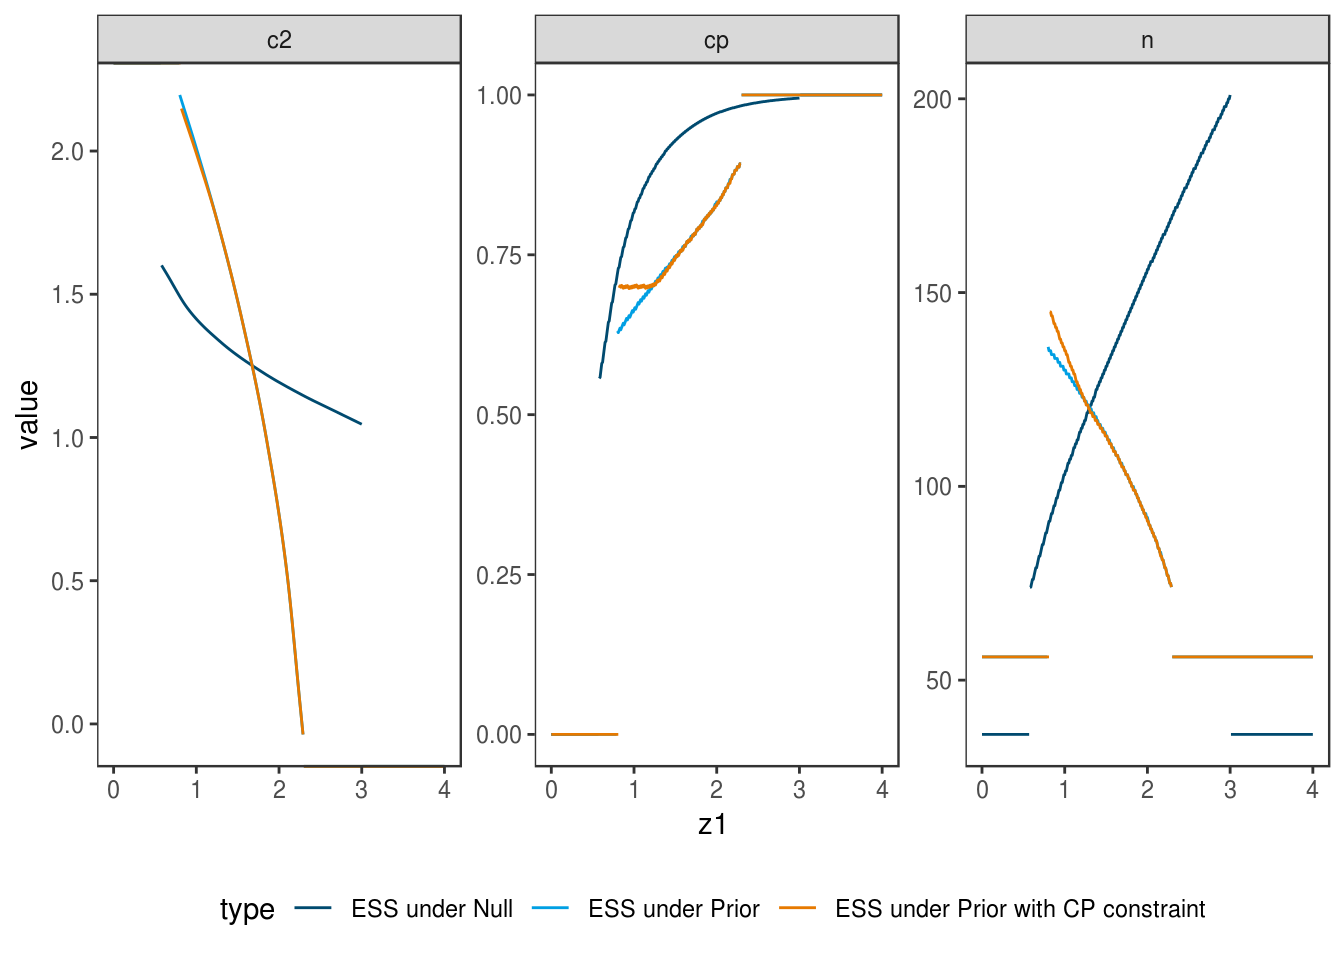
\includegraphics{adoptr-validation-report_files/figure-latex/unnamed-chunk-37-1.pdf}

\hypertarget{scenarioII}{%
\chapter{Scenario II: Large effect, Gaussian prior}\label{scenarioII}}

\hypertarget{details-1}{%
\section{Details}\label{details-1}}

In this scenario, a classical two-arm trial with normal
test statistic and known variance (w.l.o.g. variance of
the test statistic is 1).
This situation corresponds to a classical \(z\)-test for
a difference in population means.

\begin{Shaded}
\begin{Highlighting}[]
\NormalTok{datadist <-}\StringTok{ }\KeywordTok{Normal}\NormalTok{(}\DataTypeTok{two_armed =} \OtherTok{TRUE}\NormalTok{)}
\end{Highlighting}
\end{Shaded}

The null hypothesis is no population mean difference, i.e.
\(\mathcal{H}_0:\delta \leq 0\).

\begin{Shaded}
\begin{Highlighting}[]
\NormalTok{H_}\DecValTok{0}\NormalTok{ <-}\StringTok{ }\KeywordTok{PointMassPrior}\NormalTok{(.}\DecValTok{0}\NormalTok{, }\DecValTok{1}\NormalTok{)}
\end{Highlighting}
\end{Shaded}

A Gaussian prior on the effect size
\(\delta \sim \mathcal{N} ( 0.4, 0.2^2)\) is assumed.

\begin{Shaded}
\begin{Highlighting}[]
\NormalTok{prior <-}\StringTok{ }\KeywordTok{ContinuousPrior}\NormalTok{(}\ControlFlowTok{function}\NormalTok{(delta) }\KeywordTok{dnorm}\NormalTok{(delta, }\DataTypeTok{mean =} \FloatTok{.4}\NormalTok{, }\DataTypeTok{sd =} \FloatTok{.2}\NormalTok{),}
                         \DataTypeTok{support =} \KeywordTok{c}\NormalTok{(}\OperatorTok{-}\DecValTok{5}\NormalTok{, }\DecValTok{5}\NormalTok{),}
                         \DataTypeTok{tighten_support =} \OtherTok{TRUE}\NormalTok{)}
\end{Highlighting}
\end{Shaded}

Across all variants in this scenario, the one-sided maximal
type one error rate is restricted to

\begin{Shaded}
\begin{Highlighting}[]
\NormalTok{alpha <-}\StringTok{ }\FloatTok{0.025}
\end{Highlighting}
\end{Shaded}

and the power at the point alternative of \(\delta=0.4\) must
be at least

\begin{Shaded}
\begin{Highlighting}[]
\NormalTok{min_power <-}\StringTok{ }\FloatTok{0.8}
\end{Highlighting}
\end{Shaded}

I.e. throughout this sceanrio, we always use the two
constraints

\begin{Shaded}
\begin{Highlighting}[]
\NormalTok{toer_cnstr <-}\StringTok{ }\KeywordTok{expected}\NormalTok{(}\KeywordTok{ConditionalPower}\NormalTok{(datadist, H_}\DecValTok{0}\NormalTok{)) }\OperatorTok{<=}\StringTok{ }\NormalTok{alpha}
\end{Highlighting}
\end{Shaded}

and

\begin{Shaded}
\begin{Highlighting}[]
\NormalTok{pow_cnstr <-}\StringTok{ }\KeywordTok{expected}\NormalTok{(}\KeywordTok{ConditionalPower}\NormalTok{(datadist, prior)) }\OperatorTok{>=}\StringTok{ }\NormalTok{min_power}
\end{Highlighting}
\end{Shaded}

\hypertarget{variantII_1}{%
\section{Variant II-1: Minimizing Expected Sample Size under Point Prior}\label{variantII_1}}

\hypertarget{objective-3}{%
\subsection{Objective}\label{objective-3}}

Expected sample size under the prior is minimized, i.e.,
\(\boldsymbol{E}\big[n(\mathcal{D})\big]\).

\begin{Shaded}
\begin{Highlighting}[]
\NormalTok{ess <-}\StringTok{ }\KeywordTok{expected}\NormalTok{(}\KeywordTok{ConditionalSampleSize}\NormalTok{(datadist, prior))}
\end{Highlighting}
\end{Shaded}

\hypertarget{constrains-3}{%
\subsection{Constrains}\label{constrains-3}}

No additional constraints are considered in this variant.

\hypertarget{initial-design-3}{%
\subsection{Initial Design}\label{initial-design-3}}

\texttt{adoptr} requires the definition of an initial design for optimization.
We start with a group-sequential design from the package \texttt{rpact} that
fulfills the type-one error rate constraint and the power
constraint for a point effect size at \(\delta = 0.4\).
The order of integration is set to \(5\).
For usage as two-stage design with variable sample size, it has to
be converted to a \texttt{TwoStageDesign}.

\begin{Shaded}
\begin{Highlighting}[]
\NormalTok{order <-}\StringTok{ }\NormalTok{5L }

\NormalTok{init_design_gs <-}\StringTok{ }\KeywordTok{rpact_design}\NormalTok{(}\FloatTok{0.4}\NormalTok{, }\FloatTok{0.025}\NormalTok{, }\FloatTok{0.8}\NormalTok{, }\OtherTok{TRUE}\NormalTok{, order)}

\NormalTok{init_design    <-}\StringTok{ }\KeywordTok{TwoStageDesign}\NormalTok{(init_design_gs)}
\end{Highlighting}
\end{Shaded}

\hypertarget{optimization-3}{%
\subsection{Optimization}\label{optimization-3}}

The optimal design is computed in three variants: two-stage,
group-sequential, and one-stage.
The input only differs with regard to the initial design.

\begin{Shaded}
\begin{Highlighting}[]
\NormalTok{opt_design <-}\StringTok{ }\ControlFlowTok{function}\NormalTok{(initial_design) \{}
    \KeywordTok{minimize}\NormalTok{(}
\NormalTok{        ess,}
        \KeywordTok{subject_to}\NormalTok{(}
\NormalTok{            toer_cnstr,}
\NormalTok{            pow_cnstr}
\NormalTok{        ),}
        \DataTypeTok{initial_design =}\NormalTok{ initial_design,}
        \DataTypeTok{opts =}\NormalTok{ opts}
\NormalTok{    )}
\NormalTok{\}}

\NormalTok{opt1_gs <-}\StringTok{ }\KeywordTok{opt_design}\NormalTok{(init_design_gs)}
\end{Highlighting}
\end{Shaded}

\begin{verbatim}
## Warning in minimize(ess, subject_to(toer_cnstr, pow_cnstr), initial_design
## = initial_design, : initial design is infeasible!
\end{verbatim}

\begin{Shaded}
\begin{Highlighting}[]
\NormalTok{opt1_os <-}\StringTok{ }\KeywordTok{opt_design}\NormalTok{(}\KeywordTok{OneStageDesign}\NormalTok{(}\DecValTok{300}\NormalTok{, }\FloatTok{2.0}\NormalTok{))}
\NormalTok{opt1_ts <-}\StringTok{ }\KeywordTok{opt_design}\NormalTok{(}\KeywordTok{TwoStageDesign}\NormalTok{(opt1_gs}\OperatorTok{$}\NormalTok{design))}
\end{Highlighting}
\end{Shaded}

\begin{verbatim}
## Warning in minimize(ess, subject_to(toer_cnstr, pow_cnstr), initial_design
## = initial_design, : initial design is infeasible!
\end{verbatim}

\hypertarget{test-cases-3}{%
\subsection{Test Cases}\label{test-cases-3}}

Check if the optimization algorithm converged in all cases.

\begin{Shaded}
\begin{Highlighting}[]
\NormalTok{iters <-}\StringTok{ }\KeywordTok{sapply}\NormalTok{(}\KeywordTok{list}\NormalTok{(opt1_ts, opt1_gs, opt1_os), }
                \ControlFlowTok{function}\NormalTok{(x) x}\OperatorTok{$}\NormalTok{nloptr_return}\OperatorTok{$}\NormalTok{iterations)}

\KeywordTok{print}\NormalTok{(iters)}
\end{Highlighting}
\end{Shaded}

\begin{verbatim}
## [1] 1290  504   23
\end{verbatim}

\begin{Shaded}
\begin{Highlighting}[]
\NormalTok{testthat}\OperatorTok{::}\KeywordTok{expect_true}\NormalTok{(}\KeywordTok{all}\NormalTok{(iters }\OperatorTok{<}\StringTok{ }\NormalTok{opts}\OperatorTok{$}\NormalTok{maxeval))}
\end{Highlighting}
\end{Shaded}

Type one error rate constraint is tested for the three designs.

\begin{Shaded}
\begin{Highlighting}[]
\NormalTok{tmp     <-}\StringTok{ }\KeywordTok{sapply}\NormalTok{(}\KeywordTok{list}\NormalTok{(opt1_ts, opt1_gs, opt1_os),  }
                  \ControlFlowTok{function}\NormalTok{(x) }\KeywordTok{sim_pr_reject}\NormalTok{(x}\OperatorTok{$}\NormalTok{design, }\FloatTok{.0}\NormalTok{, datadist))}
\NormalTok{df_toer <-}\StringTok{ }\KeywordTok{data.frame}\NormalTok{(}
    \DataTypeTok{toer =} \KeywordTok{as.numeric}\NormalTok{(tmp[}\DecValTok{1}\NormalTok{, ]),}
    \DataTypeTok{se   =} \KeywordTok{as.numeric}\NormalTok{(tmp[}\DecValTok{2}\NormalTok{, ])}
\NormalTok{)}
\KeywordTok{rm}\NormalTok{(tmp)}

\NormalTok{testthat}\OperatorTok{::}\KeywordTok{expect_true}\NormalTok{(}\KeywordTok{all}\NormalTok{(df_toer}\OperatorTok{$}\NormalTok{toer }\OperatorTok{<=}\StringTok{ }\NormalTok{alpha }\OperatorTok{*}\StringTok{ }\NormalTok{(}\DecValTok{1} \OperatorTok{+}\StringTok{ }\NormalTok{tol)))}

\NormalTok{df_toer}
\end{Highlighting}
\end{Shaded}

\begin{verbatim}
##       toer           se
## 1 0.024989 0.0001560916
## 2 0.024907 0.0001558418
## 3 0.025116 0.0001564775
\end{verbatim}

The expected sample sizes should be ordered in a specific way.

\begin{Shaded}
\begin{Highlighting}[]
\NormalTok{testthat}\OperatorTok{::}\KeywordTok{expect_gte}\NormalTok{(}
    \KeywordTok{evaluate}\NormalTok{(ess, opt1_os}\OperatorTok{$}\NormalTok{design),}
    \KeywordTok{evaluate}\NormalTok{(ess, opt1_gs}\OperatorTok{$}\NormalTok{design)}
\NormalTok{)}

\NormalTok{testthat}\OperatorTok{::}\KeywordTok{expect_gte}\NormalTok{(}
    \KeywordTok{evaluate}\NormalTok{(ess, opt1_gs}\OperatorTok{$}\NormalTok{design),}
    \KeywordTok{evaluate}\NormalTok{(ess, opt1_ts}\OperatorTok{$}\NormalTok{design)}
\NormalTok{)}
\end{Highlighting}
\end{Shaded}

\hypertarget{variantII_2}{%
\section{Variant II-2: Minimizing Expected Sample Size under Null Hypothesis}\label{variantII_2}}

\hypertarget{objective-4}{%
\subsection{Objective}\label{objective-4}}

Expected sample size conditioned on negative effect sizes is minimized, i.e.,

\begin{Shaded}
\begin{Highlighting}[]
\NormalTok{ess_}\DecValTok{0}\NormalTok{ <-}\StringTok{ }\KeywordTok{expected}\NormalTok{(}\KeywordTok{ConditionalSampleSize}\NormalTok{(datadist, }\KeywordTok{condition}\NormalTok{(prior, }\KeywordTok{c}\NormalTok{(}\OperatorTok{-}\DecValTok{3}\NormalTok{, }\DecValTok{0}\NormalTok{))))}
\end{Highlighting}
\end{Shaded}

\hypertarget{constrains-4}{%
\subsection{Constrains}\label{constrains-4}}

No additional constraints are considered in this variant.

\hypertarget{initial-design-4}{%
\subsection{Initial Design}\label{initial-design-4}}

The previous initial design can still be applied.

\hypertarget{optimization-4}{%
\subsection{Optimization}\label{optimization-4}}

The optimal group-sequential design and based on this the
optimal two-stage design are computed.

\begin{Shaded}
\begin{Highlighting}[]
\NormalTok{opt2 <-}\StringTok{ }\ControlFlowTok{function}\NormalTok{(initial_design) \{}
    \KeywordTok{minimize}\NormalTok{(}
\NormalTok{        ess_}\DecValTok{0}\NormalTok{,}
        \KeywordTok{subject_to}\NormalTok{(}
\NormalTok{            toer_cnstr,}
\NormalTok{            pow_cnstr}
\NormalTok{        ),}
        \DataTypeTok{initial_design =}\NormalTok{ initial_design,}
        \DataTypeTok{opts =}\NormalTok{ opts}
\NormalTok{    )}
\NormalTok{\}}

\NormalTok{opt2_gs <-}\StringTok{ }\KeywordTok{opt2}\NormalTok{(init_design_gs)}
\end{Highlighting}
\end{Shaded}

\begin{verbatim}
## Warning in minimize(ess_0, subject_to(toer_cnstr, pow_cnstr),
## initial_design = initial_design, : initial design is infeasible!
\end{verbatim}

\begin{Shaded}
\begin{Highlighting}[]
\NormalTok{opt2_ts <-}\StringTok{ }\KeywordTok{opt2}\NormalTok{(}\KeywordTok{TwoStageDesign}\NormalTok{(opt2_gs}\OperatorTok{$}\NormalTok{design))}
\end{Highlighting}
\end{Shaded}

\begin{verbatim}
## Warning in minimize(ess_0, subject_to(toer_cnstr, pow_cnstr),
## initial_design = initial_design, : initial design is infeasible!
\end{verbatim}

\hypertarget{test-cases-4}{%
\subsection{Test Cases}\label{test-cases-4}}

Check if the optimization algorithm converged.

\begin{Shaded}
\begin{Highlighting}[]
\KeywordTok{print}\NormalTok{(opt2_ts}\OperatorTok{$}\NormalTok{nloptr_return}\OperatorTok{$}\NormalTok{iterations)}
\end{Highlighting}
\end{Shaded}

\begin{verbatim}
## [1] 2985
\end{verbatim}

\begin{Shaded}
\begin{Highlighting}[]
\NormalTok{testthat}\OperatorTok{::}\KeywordTok{expect_true}\NormalTok{(opt2_ts}\OperatorTok{$}\NormalTok{nloptr_return}\OperatorTok{$}\NormalTok{iterations }\OperatorTok{<}\StringTok{ }\NormalTok{opts}\OperatorTok{$}\NormalTok{maxeval)}
\end{Highlighting}
\end{Shaded}

Type one error rate constraint is tested for the optimal design.

\begin{Shaded}
\begin{Highlighting}[]
\NormalTok{tmp     <-}\StringTok{ }\KeywordTok{sim_pr_reject}\NormalTok{(opt2_ts}\OperatorTok{$}\NormalTok{design, }\FloatTok{.0}\NormalTok{, datadist)}
\NormalTok{df_toer2 <-}\StringTok{ }\KeywordTok{data.frame}\NormalTok{(}
    \DataTypeTok{toer =} \KeywordTok{as.numeric}\NormalTok{(tmp[}\DecValTok{1}\NormalTok{]),}
    \DataTypeTok{se   =} \KeywordTok{as.numeric}\NormalTok{(tmp[}\DecValTok{2}\NormalTok{])}
\NormalTok{)}
\KeywordTok{rm}\NormalTok{(tmp)}

\NormalTok{testthat}\OperatorTok{::}\KeywordTok{expect_true}\NormalTok{(}\KeywordTok{all}\NormalTok{(df_toer2}\OperatorTok{$}\NormalTok{toer }\OperatorTok{<=}\StringTok{ }\NormalTok{alpha }\OperatorTok{*}\StringTok{ }\NormalTok{(}\DecValTok{1} \OperatorTok{+}\StringTok{ }\NormalTok{tol)))}

\NormalTok{df_toer2}
\end{Highlighting}
\end{Shaded}

\begin{verbatim}
##       toer           se
## 1 0.024858 0.0001556923
\end{verbatim}

The expected sample size under the null hypothesis should be lower
than of the design from variant II.1 where expected sample size under
the full prior was minimized.

\begin{Shaded}
\begin{Highlighting}[]
\NormalTok{testthat}\OperatorTok{::}\KeywordTok{expect_lte}\NormalTok{(}
    \KeywordTok{evaluate}\NormalTok{(ess_}\DecValTok{0}\NormalTok{, opt2_ts}\OperatorTok{$}\NormalTok{design),}
    \KeywordTok{evaluate}\NormalTok{(ess_}\DecValTok{0}\NormalTok{, opt1_ts}\OperatorTok{$}\NormalTok{design)}
\NormalTok{)}
\end{Highlighting}
\end{Shaded}

\hypertarget{variantII_3}{%
\section{Variant II-3: Conditional Power Constraint}\label{variantII_3}}

\hypertarget{objective-5}{%
\subsection{Objective}\label{objective-5}}

Expected sample size under the prior is minimized and has already been defined.

\hypertarget{constrains-5}{%
\subsection{Constrains}\label{constrains-5}}

The constraints remain the same as before, additionally to a constraint
on conditional power.

\begin{Shaded}
\begin{Highlighting}[]
\NormalTok{cp <-}\StringTok{ }\KeywordTok{ConditionalPower}\NormalTok{(datadist, }\KeywordTok{condition}\NormalTok{(prior, }\KeywordTok{c}\NormalTok{(}\DecValTok{0}\NormalTok{, }\DecValTok{3}\NormalTok{)))}

\NormalTok{cp_cnstr <-}\StringTok{ }\NormalTok{cp }\OperatorTok{>=}\StringTok{ }\FloatTok{.7}
\end{Highlighting}
\end{Shaded}

\hypertarget{initial-design-5}{%
\subsection{Initial Design}\label{initial-design-5}}

The previous initial design can still be applied.

\hypertarget{optimization-5}{%
\subsection{Optimization}\label{optimization-5}}

The optimal two-stage design is computed.

\begin{Shaded}
\begin{Highlighting}[]
\NormalTok{opt3_ts <-}\StringTok{ }\KeywordTok{minimize}\NormalTok{(}
\NormalTok{        ess,}
        \KeywordTok{subject_to}\NormalTok{(}
\NormalTok{            toer_cnstr,}
\NormalTok{            pow_cnstr,}
\NormalTok{            cp_cnstr}
\NormalTok{        ),}
        \DataTypeTok{initial_design =}\NormalTok{ init_design,}
        \DataTypeTok{opts =}\NormalTok{ opts}
\NormalTok{)}
\end{Highlighting}
\end{Shaded}

\begin{verbatim}
## Warning in minimize(ess, subject_to(toer_cnstr, pow_cnstr, cp_cnstr),
## initial_design = init_design, : initial design is infeasible!
\end{verbatim}

\hypertarget{test-cases-5}{%
\subsection{Test Cases}\label{test-cases-5}}

Check if the optimization algorithm converged.

\begin{Shaded}
\begin{Highlighting}[]
\KeywordTok{print}\NormalTok{(opt3_ts}\OperatorTok{$}\NormalTok{nloptr_return}\OperatorTok{$}\NormalTok{iterations)}
\end{Highlighting}
\end{Shaded}

\begin{verbatim}
## [1] 3040
\end{verbatim}

\begin{Shaded}
\begin{Highlighting}[]
\NormalTok{testthat}\OperatorTok{::}\KeywordTok{expect_true}\NormalTok{(opt3_ts}\OperatorTok{$}\NormalTok{nloptr_return}\OperatorTok{$}\NormalTok{iterations }\OperatorTok{<}\StringTok{ }\NormalTok{opts}\OperatorTok{$}\NormalTok{maxeval)}
\end{Highlighting}
\end{Shaded}

Type one error rate constraint is tested for the optimal design.

\begin{Shaded}
\begin{Highlighting}[]
\NormalTok{tmp     <-}\StringTok{ }\KeywordTok{sim_pr_reject}\NormalTok{(opt3_ts}\OperatorTok{$}\NormalTok{design, }\FloatTok{.0}\NormalTok{, datadist)}
\NormalTok{df_toer3 <-}\StringTok{ }\KeywordTok{data.frame}\NormalTok{(}
    \DataTypeTok{toer =} \KeywordTok{as.numeric}\NormalTok{(tmp[}\DecValTok{1}\NormalTok{]),}
    \DataTypeTok{se   =} \KeywordTok{as.numeric}\NormalTok{(tmp[}\DecValTok{2}\NormalTok{])}
\NormalTok{)}
\KeywordTok{rm}\NormalTok{(tmp)}

\NormalTok{testthat}\OperatorTok{::}\KeywordTok{expect_true}\NormalTok{(}\KeywordTok{all}\NormalTok{(df_toer3}\OperatorTok{$}\NormalTok{toer }\OperatorTok{<=}\StringTok{ }\NormalTok{alpha }\OperatorTok{*}\StringTok{ }\NormalTok{(}\DecValTok{1} \OperatorTok{+}\StringTok{ }\NormalTok{tol)))}

\NormalTok{df_toer3}
\end{Highlighting}
\end{Shaded}

\begin{verbatim}
##       toer           se
## 1 0.025016 0.0001561737
\end{verbatim}

The conditional power constraint needs to be tested.
Select three points for this and check the constraint.

\begin{Shaded}
\begin{Highlighting}[]
\NormalTok{x <-}\StringTok{ }\NormalTok{adoptr}\OperatorTok{:::}\KeywordTok{scaled_integration_pivots}\NormalTok{(opt3_ts}\OperatorTok{$}\NormalTok{design)[}\KeywordTok{c}\NormalTok{(}\DecValTok{1}\NormalTok{, }\DecValTok{3}\NormalTok{, }\DecValTok{5}\NormalTok{)]}

\NormalTok{cp_val <-}\StringTok{ }\KeywordTok{sapply}\NormalTok{(x, }\ControlFlowTok{function}\NormalTok{(z) }\KeywordTok{evaluate}\NormalTok{(cp, opt3_ts}\OperatorTok{$}\NormalTok{design, z))}

\NormalTok{testthat}\OperatorTok{::}\KeywordTok{expect_true}\NormalTok{(}\KeywordTok{all}\NormalTok{(cp_val }\OperatorTok{>=}\StringTok{ }\FloatTok{0.7} \OperatorTok{*}\StringTok{ }\NormalTok{(}\DecValTok{1} \OperatorTok{-}\StringTok{ }\NormalTok{tol)))}
\end{Highlighting}
\end{Shaded}

The expected sample size under the prior should be higher than
in the case without the constraint that was analyzed in II.1.

\begin{Shaded}
\begin{Highlighting}[]
\NormalTok{testthat}\OperatorTok{::}\KeywordTok{expect_gte}\NormalTok{(}
    \KeywordTok{evaluate}\NormalTok{(ess, opt3_ts}\OperatorTok{$}\NormalTok{design),}
    \KeywordTok{evaluate}\NormalTok{(ess, opt1_ts}\OperatorTok{$}\NormalTok{design)}
\NormalTok{)}
\end{Highlighting}
\end{Shaded}

\hypertarget{plot-two-stage-designs-1}{%
\section{Plot Two-Stage Designs}\label{plot-two-stage-designs-1}}

The optimal two-stage designs stemming from the different variants
are plotted together.

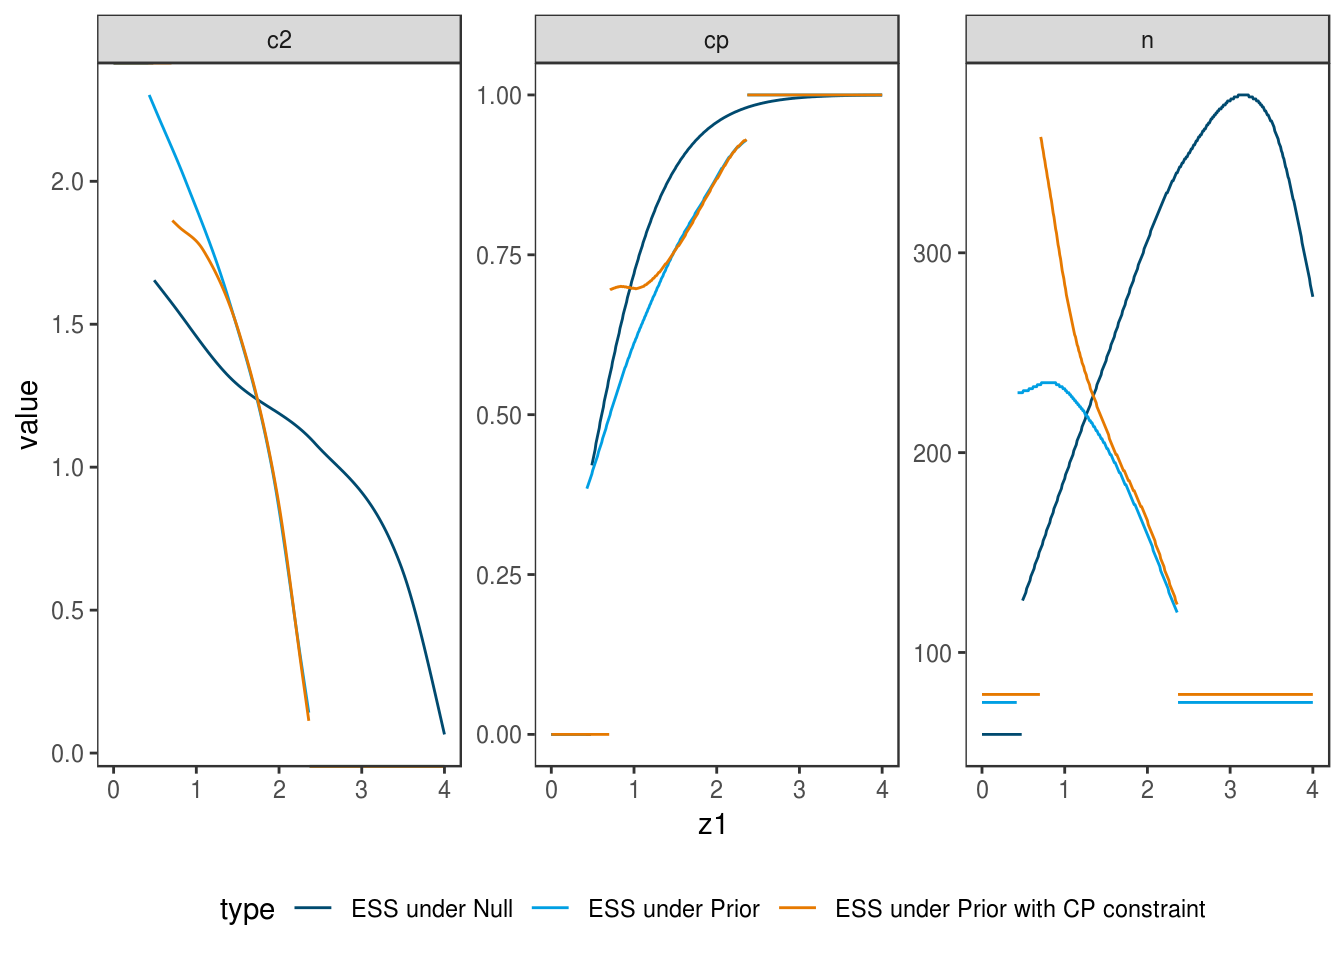
\includegraphics{adoptr-validation-report_files/figure-latex/unnamed-chunk-62-1.pdf}

\hypertarget{scenarioIII}{%
\chapter{Scenario III: large effect, uniform prior}\label{scenarioIII}}

\hypertarget{details-2}{%
\section{Details}\label{details-2}}

This scenario is a variant of Scenario I.
The purpose is to asses whether placing uniform priors with decreasing
width of support centered at the \(\delta=0.4\) leads to a sequence of
optimal designs which converges towards the solution in Case I-1.

\begin{Shaded}
\begin{Highlighting}[]
\NormalTok{datadist <-}\StringTok{ }\KeywordTok{Normal}\NormalTok{(}\DataTypeTok{two_armed =} \OtherTok{TRUE}\NormalTok{)}
\end{Highlighting}
\end{Shaded}

The null hypothesis is no population mean difference, i.e.
\(\mathcal{H}_0:\delta \leq 0\).

\begin{Shaded}
\begin{Highlighting}[]
\NormalTok{H_}\DecValTok{0}\NormalTok{ <-}\StringTok{ }\KeywordTok{PointMassPrior}\NormalTok{(.}\DecValTok{0}\NormalTok{, }\DecValTok{1}\NormalTok{)}
\end{Highlighting}
\end{Shaded}

In this scenario we consider a sequence of uniform distributions
\(\delta\sim\operatorname{Unif}(0.4 - \Delta_i, 0.4 + \Delta_i)\)
around \(0.4\) with \(\Delta_i=(3 - i)/10\) for \(i=0\ldots 3\).
I.e., for \(\Delta_3=0\) reduces to \texttt{PointMassPrior} on \(\delta=0.4\).

\begin{Shaded}
\begin{Highlighting}[]
\NormalTok{prior <-}\StringTok{ }\ControlFlowTok{function}\NormalTok{(delta) \{}
    \ControlFlowTok{if}\NormalTok{ (delta }\OperatorTok{==}\StringTok{ }\DecValTok{0}\NormalTok{)}
        \KeywordTok{return}\NormalTok{(}\KeywordTok{PointMassPrior}\NormalTok{(.}\DecValTok{4}\NormalTok{, }\FloatTok{1.0}\NormalTok{))}
\NormalTok{    a <-}\StringTok{ }\FloatTok{.4} \OperatorTok{-}\StringTok{ }\NormalTok{delta; b <-}\StringTok{ }\FloatTok{.4} \OperatorTok{+}\StringTok{ }\NormalTok{delta}
    \KeywordTok{ContinuousPrior}\NormalTok{(}\ControlFlowTok{function}\NormalTok{(x) }\KeywordTok{dunif}\NormalTok{(x, a, b), }\DataTypeTok{support =} \KeywordTok{c}\NormalTok{(a, b))}
\NormalTok{\}}
\end{Highlighting}
\end{Shaded}

Across all variants in this scenario, the one-sided maximal
type one error rate is restricted to

\begin{Shaded}
\begin{Highlighting}[]
\NormalTok{alpha <-}\StringTok{ }\FloatTok{0.025}
\end{Highlighting}
\end{Shaded}

and the expected power at the point alternative of \(\delta=0.4\) must
be at least

\begin{Shaded}
\begin{Highlighting}[]
\NormalTok{min_power <-}\StringTok{ }\FloatTok{0.8}
\end{Highlighting}
\end{Shaded}

I.e. throughout this sceanrio, we always use the two
constraints

\begin{Shaded}
\begin{Highlighting}[]
\NormalTok{toer_cnstr <-}\StringTok{ }\KeywordTok{expected}\NormalTok{(}\KeywordTok{ConditionalPower}\NormalTok{(datadist, H_}\DecValTok{0}\NormalTok{)) }\OperatorTok{<=}\StringTok{ }\NormalTok{alpha}
\end{Highlighting}
\end{Shaded}

and

\begin{Shaded}
\begin{Highlighting}[]
\NormalTok{ep_cnstr <-}\StringTok{ }\ControlFlowTok{function}\NormalTok{(delta) \{}
\NormalTok{    prior     <-}\StringTok{ }\KeywordTok{prior}\NormalTok{(delta)}
\NormalTok{    cnd_prior <-}\StringTok{ }\KeywordTok{condition}\NormalTok{(prior, }\KeywordTok{c}\NormalTok{(}\DecValTok{0}\NormalTok{, }\KeywordTok{bounds}\NormalTok{(prior)[}\DecValTok{2}\NormalTok{]))}
    \KeywordTok{return}\NormalTok{( }\KeywordTok{expected}\NormalTok{(}\KeywordTok{ConditionalPower}\NormalTok{(datadist, cnd_prior)) }\OperatorTok{>=}\StringTok{ }\FloatTok{0.8}\NormalTok{ )}
\NormalTok{\}}
\end{Highlighting}
\end{Shaded}

\hypertarget{variantIII_1}{%
\section{Variant III.1: Convergence under prior concentration}\label{variantIII_1}}

Make sure that the optimal solution converges as the prior is more and more
concentrated at a point mass.

\hypertarget{objective-6}{%
\subsection{Objective}\label{objective-6}}

Expected sample size under the respective prior is minimized, i.e.,
\(\boldsymbol{E}\big[n(\mathcal{D})\big]\).

\begin{Shaded}
\begin{Highlighting}[]
\NormalTok{objective <-}\StringTok{ }\ControlFlowTok{function}\NormalTok{(delta) \{}
    \KeywordTok{expected}\NormalTok{(}\KeywordTok{ConditionalSampleSize}\NormalTok{(datadist, }\KeywordTok{prior}\NormalTok{(delta)))}
\NormalTok{\}}
\end{Highlighting}
\end{Shaded}

\hypertarget{constrains-6}{%
\subsection{Constrains}\label{constrains-6}}

The constraints have already been described under details.

\hypertarget{optimization-problem}{%
\subsection{Optimization problem}\label{optimization-problem}}

The optimization problem depending on \(\Delta_i\) is defined below.
The default optimization paramters, 5 pivot points, and a fixed initial design
is used.
The initial design is chosen such that the error constraints are
fulfilled. Early stopping for futility is applied if the effect shows
in the opponent direction to the alternative, i.e. \(c_1^f=0\).
\(c_2\) is chosen close to and \(c_1^e\) a little larger than the \(1-\alpha\)-quantile
of the standard normal distribution. The sample sizes are selected
to fulfill the error constraints.

\begin{Shaded}
\begin{Highlighting}[]
\NormalTok{init <-}\StringTok{ }\KeywordTok{TwoStageDesign}\NormalTok{(}
    \DataTypeTok{n1    =} \DecValTok{150}\NormalTok{,}
    \DataTypeTok{c1f   =} \DecValTok{0}\NormalTok{,}
    \DataTypeTok{c1e   =} \FloatTok{2.3}\NormalTok{,}
    \DataTypeTok{n2    =} \FloatTok{125.0}\NormalTok{,}
    \DataTypeTok{c2    =} \FloatTok{2.0}\NormalTok{,}
    \DataTypeTok{order =} \DecValTok{5}
\NormalTok{)}

\NormalTok{optimal_design <-}\StringTok{ }\ControlFlowTok{function}\NormalTok{(delta) \{}
    \KeywordTok{minimize}\NormalTok{(}
        \KeywordTok{objective}\NormalTok{(delta),}
        \KeywordTok{subject_to}\NormalTok{(}
\NormalTok{            toer_cnstr,}
            \KeywordTok{ep_cnstr}\NormalTok{(delta)}
\NormalTok{        ),}
        \DataTypeTok{initial_design =}\NormalTok{ init}
\NormalTok{    )}
\NormalTok{\}}
\end{Highlighting}
\end{Shaded}

Compute the sequence of optimal designs

\begin{Shaded}
\begin{Highlighting}[]
\NormalTok{deltas  <-}\StringTok{ }\DecValTok{3}\OperatorTok{:}\DecValTok{0}\OperatorTok{/}\DecValTok{10}
\NormalTok{results <-}\StringTok{ }\KeywordTok{lapply}\NormalTok{(deltas, optimal_design)}
\end{Highlighting}
\end{Shaded}

\hypertarget{test-cases-6}{%
\subsection{Test cases}\label{test-cases-6}}

Check that iteration limit was not exceeded in any case.

\begin{Shaded}
\begin{Highlighting}[]
\NormalTok{iters <-}\StringTok{ }\KeywordTok{sapply}\NormalTok{(results, }\ControlFlowTok{function}\NormalTok{(x) x}\OperatorTok{$}\NormalTok{nloptr_return}\OperatorTok{$}\NormalTok{iterations)}

\KeywordTok{print}\NormalTok{(iters)}
\end{Highlighting}
\end{Shaded}

\begin{verbatim}
## [1] 1746 1857 2438 2684
\end{verbatim}

\begin{Shaded}
\begin{Highlighting}[]
\NormalTok{testthat}\OperatorTok{::}\KeywordTok{expect_true}\NormalTok{(}\KeywordTok{all}\NormalTok{(iters }\OperatorTok{<=}\StringTok{ }\DecValTok{10000}\NormalTok{))}
\end{Highlighting}
\end{Shaded}

Check type one error rate control

\begin{Shaded}
\begin{Highlighting}[]
\NormalTok{tmp     <-}\StringTok{ }\KeywordTok{sapply}\NormalTok{(results, }\ControlFlowTok{function}\NormalTok{(x) }\KeywordTok{sim_pr_reject}\NormalTok{(x}\OperatorTok{$}\NormalTok{design, }\FloatTok{.0}\NormalTok{, datadist))}
\NormalTok{df_toer <-}\StringTok{ }\KeywordTok{data.frame}\NormalTok{(}
    \DataTypeTok{toer =} \KeywordTok{as.numeric}\NormalTok{(tmp[}\DecValTok{1}\NormalTok{, ]),}
    \DataTypeTok{se   =} \KeywordTok{as.numeric}\NormalTok{(tmp[}\DecValTok{2}\NormalTok{, ])}
\NormalTok{)}
\KeywordTok{rm}\NormalTok{(tmp)}

\NormalTok{testthat}\OperatorTok{::}\KeywordTok{expect_true}\NormalTok{(}\KeywordTok{all}\NormalTok{(df_toer}\OperatorTok{$}\NormalTok{toer }\OperatorTok{<=}\StringTok{ }\NormalTok{alpha }\OperatorTok{*}\StringTok{ }\NormalTok{(}\DecValTok{1} \OperatorTok{+}\StringTok{ }\NormalTok{tol)))}

\NormalTok{df_toer}
\end{Highlighting}
\end{Shaded}

\begin{verbatim}
##       toer           se
## 1 0.024979 0.0001560611
## 2 0.024957 0.0001559941
## 3 0.024972 0.0001560398
## 4 0.024979 0.0001560611
\end{verbatim}

Check that expected sample size decreases with decreasing prior variance.

\begin{Shaded}
\begin{Highlighting}[]
\NormalTok{testthat}\OperatorTok{::}\KeywordTok{expect_gte}\NormalTok{(}
  \KeywordTok{evaluate}\NormalTok{(}\KeywordTok{objective}\NormalTok{(deltas[}\DecValTok{1}\NormalTok{]), results[[}\DecValTok{1}\NormalTok{]]}\OperatorTok{$}\NormalTok{design),}
  \KeywordTok{evaluate}\NormalTok{(}\KeywordTok{objective}\NormalTok{(deltas[}\DecValTok{2}\NormalTok{]), results[[}\DecValTok{2}\NormalTok{]]}\OperatorTok{$}\NormalTok{design)}
\NormalTok{)}

\NormalTok{testthat}\OperatorTok{::}\KeywordTok{expect_gte}\NormalTok{(}
  \KeywordTok{evaluate}\NormalTok{(}\KeywordTok{objective}\NormalTok{(deltas[}\DecValTok{2}\NormalTok{]), results[[}\DecValTok{2}\NormalTok{]]}\OperatorTok{$}\NormalTok{design),}
  \KeywordTok{evaluate}\NormalTok{(}\KeywordTok{objective}\NormalTok{(deltas[}\DecValTok{3}\NormalTok{]), results[[}\DecValTok{3}\NormalTok{]]}\OperatorTok{$}\NormalTok{design)}
\NormalTok{)}

\NormalTok{testthat}\OperatorTok{::}\KeywordTok{expect_gte}\NormalTok{(}
  \KeywordTok{evaluate}\NormalTok{(}\KeywordTok{objective}\NormalTok{(deltas[}\DecValTok{3}\NormalTok{]), results[[}\DecValTok{3}\NormalTok{]]}\OperatorTok{$}\NormalTok{design),}
  \KeywordTok{evaluate}\NormalTok{(}\KeywordTok{objective}\NormalTok{(deltas[}\DecValTok{4}\NormalTok{]), results[[}\DecValTok{4}\NormalTok{]]}\OperatorTok{$}\NormalTok{design)}
\NormalTok{)}
\end{Highlighting}
\end{Shaded}

\hypertarget{plot-designs}{%
\subsection{Plot designs}\label{plot-designs}}

Plot and assess for convergence

\begin{Shaded}
\begin{Highlighting}[]
\NormalTok{z1 <-}\StringTok{ }\KeywordTok{seq}\NormalTok{(}\DecValTok{0}\NormalTok{, }\DecValTok{3}\NormalTok{, }\DataTypeTok{by =} \FloatTok{.01}\NormalTok{)}

\KeywordTok{tibble}\NormalTok{(}
    \DataTypeTok{delta  =}\NormalTok{ deltas, }
    \DataTypeTok{design =} \KeywordTok{lapply}\NormalTok{(results, }\ControlFlowTok{function}\NormalTok{(x) x}\OperatorTok{$}\NormalTok{design)}
\NormalTok{) }\OperatorTok\StringTok{ }
\StringTok{    }\KeywordTok{group_by}\NormalTok{(delta) }\OperatorTok\StringTok{ }
\StringTok{    }\KeywordTok{do}\NormalTok{(}
        \DataTypeTok{z1 =}\NormalTok{ z1,}
        \DataTypeTok{n  =}\NormalTok{ adoptr}\OperatorTok{::}\KeywordTok{n}\NormalTok{(.}\OperatorTok{$}\NormalTok{design[[}\DecValTok{1}\NormalTok{]], z1),}
        \DataTypeTok{c2 =} \KeywordTok{c2}\NormalTok{(.}\OperatorTok{$}\NormalTok{design[[}\DecValTok{1}\NormalTok{]], z1)}
\NormalTok{    ) }\OperatorTok\StringTok{ }
\StringTok{    }\KeywordTok{unnest}\NormalTok{() }\OperatorTok\StringTok{ }
\StringTok{    }\KeywordTok{mutate}\NormalTok{(}
        \DataTypeTok{section =} \KeywordTok{ifelse}\NormalTok{(}
            \KeywordTok{is.finite}\NormalTok{(c2), }
            \StringTok{"continuation"}\NormalTok{, }
            \KeywordTok{ifelse}\NormalTok{(c2 }\OperatorTok{==}\StringTok{ }\OperatorTok{-}\OtherTok{Inf}\NormalTok{, }\StringTok{"efficacy"}\NormalTok{, }\StringTok{"futility"}\NormalTok{)}
\NormalTok{        )}
\NormalTok{    ) }\OperatorTok\StringTok{ }
\StringTok{    }\KeywordTok{gather}\NormalTok{(variable, value, n, c2) }\OperatorTok\StringTok{ }
\StringTok{    }\KeywordTok{ggplot}\NormalTok{(}\KeywordTok{aes}\NormalTok{(z1, value, }\DataTypeTok{color =}\NormalTok{ delta)) }\OperatorTok{+}
\StringTok{        }\KeywordTok{geom_line}\NormalTok{(}\KeywordTok{aes}\NormalTok{(}\DataTypeTok{group =} \KeywordTok{interaction}\NormalTok{(section, delta))) }\OperatorTok{+}\StringTok{ }
\StringTok{        }\KeywordTok{facet_wrap}\NormalTok{(}\OperatorTok{~}\NormalTok{variable, }\DataTypeTok{scales =} \StringTok{"free_y"}\NormalTok{) }\OperatorTok{+}
\StringTok{        }\KeywordTok{theme_bw}\NormalTok{() }\OperatorTok{+}
\StringTok{        }\KeywordTok{scale_color_continuous}\NormalTok{(}\KeywordTok{bquote}\NormalTok{(Delta)) }\OperatorTok{+}
\StringTok{        }\KeywordTok{theme}\NormalTok{(}
            \DataTypeTok{panel.grid =} \KeywordTok{element_blank}\NormalTok{(),}
            \DataTypeTok{legend.position =} \StringTok{"bottom"}
\NormalTok{        )}
\end{Highlighting}
\end{Shaded}

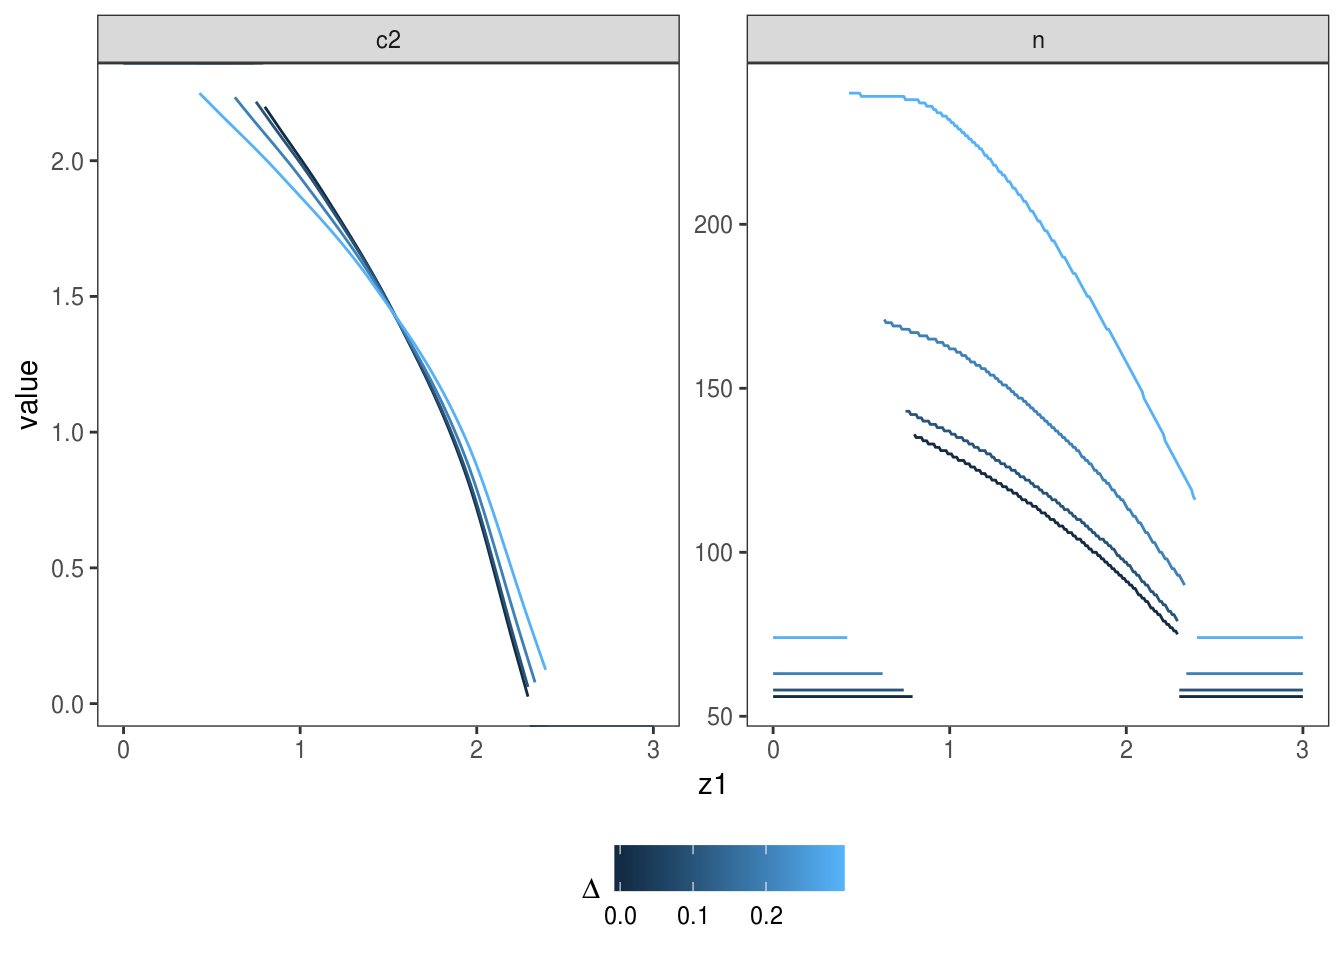
\includegraphics{adoptr-validation-report_files/figure-latex/unnamed-chunk-76-1.pdf}

\hypertarget{scenarioIV}{%
\chapter{Scenario IV: smaller effect, point prior}\label{scenarioIV}}

\hypertarget{details-3}{%
\section{Details}\label{details-3}}

In this scenario, a classical two-arm trial with normal
test statistic and known variance (w.l.o.g. variance of
the test statistic is 1).
This situation corresponds to a classical \(z\)-test for
a difference in population means.

\begin{Shaded}
\begin{Highlighting}[]
\NormalTok{datadist <-}\StringTok{ }\KeywordTok{Normal}\NormalTok{(}\DataTypeTok{two_armed =} \OtherTok{TRUE}\NormalTok{)}
\end{Highlighting}
\end{Shaded}

The null hypothesis is no population mean difference, i.e.
\(\mathcal{H}_0:\delta \leq 0\).

\begin{Shaded}
\begin{Highlighting}[]
\NormalTok{H_}\DecValTok{0}\NormalTok{ <-}\StringTok{ }\KeywordTok{PointMassPrior}\NormalTok{(.}\DecValTok{0}\NormalTok{, }\DecValTok{1}\NormalTok{)}
\end{Highlighting}
\end{Shaded}

An alternative effect size of \(\delta = 0.2\) with
point prior distribution is assumed.

\begin{Shaded}
\begin{Highlighting}[]
\NormalTok{prior <-}\StringTok{ }\KeywordTok{PointMassPrior}\NormalTok{(.}\DecValTok{2}\NormalTok{, }\DecValTok{1}\NormalTok{)}
\end{Highlighting}
\end{Shaded}

Across all variants in this scenario, the one-sided maximal
type one error rate is restricted to

\begin{Shaded}
\begin{Highlighting}[]
\NormalTok{alpha <-}\StringTok{ }\FloatTok{0.025}
\end{Highlighting}
\end{Shaded}

and the power at the point alternative of \(\delta=0.2\) must
be at least

\begin{Shaded}
\begin{Highlighting}[]
\NormalTok{min_power <-}\StringTok{ }\FloatTok{0.8}
\end{Highlighting}
\end{Shaded}

I.e. throughout this sceanrio, we always use the two
constraints

\begin{Shaded}
\begin{Highlighting}[]
\NormalTok{toer_cnstr <-}\StringTok{ }\KeywordTok{expected}\NormalTok{(}\KeywordTok{ConditionalPower}\NormalTok{(datadist, H_}\DecValTok{0}\NormalTok{)) }\OperatorTok{<=}\StringTok{ }\NormalTok{alpha}
\end{Highlighting}
\end{Shaded}

and

\begin{Shaded}
\begin{Highlighting}[]
\NormalTok{pow_cnstr <-}\StringTok{ }\KeywordTok{expected}\NormalTok{(}\KeywordTok{ConditionalPower}\NormalTok{(datadist, prior)) }\OperatorTok{>=}\StringTok{ }\NormalTok{min_power}
\end{Highlighting}
\end{Shaded}

\hypertarget{variantIV_1}{%
\section{Variant IV-1: Minimizing Expected Sample Size under Point Prior}\label{variantIV_1}}

\hypertarget{objective-7}{%
\subsection{Objective}\label{objective-7}}

Expected sample size under the respective prior is minimized, i.e.,
\(\boldsymbol{E}\big[n(\mathcal{D})\big]\).

\begin{Shaded}
\begin{Highlighting}[]
\NormalTok{ess <-}\StringTok{ }\KeywordTok{expected}\NormalTok{(}\KeywordTok{ConditionalSampleSize}\NormalTok{(datadist, prior))}
\end{Highlighting}
\end{Shaded}

\hypertarget{constrains-7}{%
\subsection{Constrains}\label{constrains-7}}

No additional constraints are considered in this variant.

\hypertarget{initial-design-6}{%
\subsection{Initial Design}\label{initial-design-6}}

\texttt{adoptr} requires the definition of an initial design for optimization.
We start with a group-sequential design from the package \texttt{rpact} that
fulfills these constraints and is used later for comparison.
The order of integration is set to \(5\).

\begin{Shaded}
\begin{Highlighting}[]
\NormalTok{order <-}\StringTok{ }\NormalTok{5L }

\NormalTok{init_design_gs <-}\StringTok{ }\KeywordTok{rpact_design}\NormalTok{(}\FloatTok{0.2}\NormalTok{, }\FloatTok{0.025}\NormalTok{, }\FloatTok{0.8}\NormalTok{, }\OtherTok{TRUE}\NormalTok{, order)}
\end{Highlighting}
\end{Shaded}

\hypertarget{optimization-6}{%
\subsection{Optimization}\label{optimization-6}}

The optimal design is computed in three variants: two-stage, group-sequential
and one-stage.
The input only differs with regard to the initial design.
The optimal group-sequential design is used as initial design to
compute the optimal two-stage design.

\begin{Shaded}
\begin{Highlighting}[]
\NormalTok{opt_design <-}\StringTok{ }\ControlFlowTok{function}\NormalTok{(initial_design) \{}
    \KeywordTok{minimize}\NormalTok{(}
\NormalTok{        ess,}
        \KeywordTok{subject_to}\NormalTok{(}
\NormalTok{            toer_cnstr,}
\NormalTok{            pow_cnstr}
\NormalTok{        ),}
        \DataTypeTok{initial_design =}\NormalTok{ initial_design,}
        \DataTypeTok{opts =}\NormalTok{ opts}
\NormalTok{    )}
\NormalTok{\}}

\NormalTok{opt1_gs <-}\StringTok{ }\KeywordTok{opt_design}\NormalTok{(init_design_gs)}
\NormalTok{opt1_ts <-}\StringTok{ }\KeywordTok{opt_design}\NormalTok{(}\KeywordTok{TwoStageDesign}\NormalTok{(opt1_gs}\OperatorTok{$}\NormalTok{design))}
\end{Highlighting}
\end{Shaded}

\begin{verbatim}
## Warning in minimize(ess, subject_to(toer_cnstr, pow_cnstr), initial_design
## = initial_design, : initial design is infeasible!
\end{verbatim}

\begin{Shaded}
\begin{Highlighting}[]
\NormalTok{opt1_os <-}\StringTok{ }\KeywordTok{opt_design}\NormalTok{(}\KeywordTok{OneStageDesign}\NormalTok{(}\DecValTok{500}\NormalTok{, }\FloatTok{2.0}\NormalTok{))}
\end{Highlighting}
\end{Shaded}

\hypertarget{test-cases-7}{%
\subsection{Test Cases}\label{test-cases-7}}

Check if the optimization algorithm converged in all cases.

\begin{Shaded}
\begin{Highlighting}[]
\NormalTok{iters <-}\StringTok{ }\KeywordTok{sapply}\NormalTok{(}\KeywordTok{list}\NormalTok{(opt1_ts, opt1_gs, opt1_os), }
                \ControlFlowTok{function}\NormalTok{(x) x}\OperatorTok{$}\NormalTok{nloptr_return}\OperatorTok{$}\NormalTok{iterations)}

\KeywordTok{print}\NormalTok{(iters)}
\end{Highlighting}
\end{Shaded}

\begin{verbatim}
## [1] 1960  912   20
\end{verbatim}

\begin{Shaded}
\begin{Highlighting}[]
\NormalTok{testthat}\OperatorTok{::}\KeywordTok{expect_true}\NormalTok{(}\KeywordTok{all}\NormalTok{(iters }\OperatorTok{<}\StringTok{ }\NormalTok{opts}\OperatorTok{$}\NormalTok{maxeval))}
\end{Highlighting}
\end{Shaded}

Type one error rate constraint is tested for the three designs.

\begin{Shaded}
\begin{Highlighting}[]
\NormalTok{tmp     <-}\StringTok{ }\KeywordTok{sapply}\NormalTok{(}\KeywordTok{list}\NormalTok{(opt1_ts, opt1_gs, opt1_os),  }
                  \ControlFlowTok{function}\NormalTok{(x) }\KeywordTok{sim_pr_reject}\NormalTok{(x}\OperatorTok{$}\NormalTok{design, }\FloatTok{.0}\NormalTok{, datadist))}
\NormalTok{df_toer <-}\StringTok{ }\KeywordTok{data.frame}\NormalTok{(}
    \DataTypeTok{toer =} \KeywordTok{as.numeric}\NormalTok{(tmp[}\DecValTok{1}\NormalTok{, ]),}
    \DataTypeTok{se   =} \KeywordTok{as.numeric}\NormalTok{(tmp[}\DecValTok{2}\NormalTok{, ])}
\NormalTok{)}
\KeywordTok{rm}\NormalTok{(tmp)}

\NormalTok{testthat}\OperatorTok{::}\KeywordTok{expect_true}\NormalTok{(}\KeywordTok{all}\NormalTok{(df_toer}\OperatorTok{$}\NormalTok{toer }\OperatorTok{<=}\StringTok{ }\NormalTok{alpha }\OperatorTok{*}\StringTok{ }\NormalTok{(}\DecValTok{1} \OperatorTok{+}\StringTok{ }\NormalTok{tol)))}

\NormalTok{df_toer}
\end{Highlighting}
\end{Shaded}

\begin{verbatim}
##       toer           se
## 1 0.024975 0.0001560489
## 2 0.024978 0.0001560581
## 3 0.025116 0.0001564775
\end{verbatim}

The power constraint can also be tested via simulation.

\begin{Shaded}
\begin{Highlighting}[]
\NormalTok{tmp     <-}\StringTok{ }\KeywordTok{sapply}\NormalTok{(}\KeywordTok{list}\NormalTok{(opt1_ts, opt1_gs, opt1_os),  }
                  \ControlFlowTok{function}\NormalTok{(x) }\KeywordTok{sim_pr_reject}\NormalTok{(x}\OperatorTok{$}\NormalTok{design, }\FloatTok{.2}\NormalTok{, datadist))}
\NormalTok{df_pow  <-}\StringTok{ }\KeywordTok{data.frame}\NormalTok{(}
    \DataTypeTok{pow  =} \KeywordTok{as.numeric}\NormalTok{(tmp[}\DecValTok{1}\NormalTok{, ]),}
    \DataTypeTok{se   =} \KeywordTok{as.numeric}\NormalTok{(tmp[}\DecValTok{2}\NormalTok{, ])}
\NormalTok{)}
\KeywordTok{rm}\NormalTok{(tmp)}

\NormalTok{testthat}\OperatorTok{::}\KeywordTok{expect_true}\NormalTok{(}\KeywordTok{all}\NormalTok{(df_pow}\OperatorTok{$}\NormalTok{pow }\OperatorTok{>=}\StringTok{ }\NormalTok{min_power }\OperatorTok{*}\StringTok{ }\NormalTok{(}\DecValTok{1} \OperatorTok{-}\StringTok{ }\NormalTok{tol)))}

\NormalTok{df_pow}
\end{Highlighting}
\end{Shaded}

\begin{verbatim}
##        pow           se
## 1 0.799799 0.0004001509
## 2 0.799670 0.0004002475
## 3 0.799317 0.0004005115
\end{verbatim}

The expected sample sizes should be ordered in a specific way.

\begin{Shaded}
\begin{Highlighting}[]
\NormalTok{testthat}\OperatorTok{::}\KeywordTok{expect_gte}\NormalTok{(}
    \KeywordTok{evaluate}\NormalTok{(ess, opt1_os}\OperatorTok{$}\NormalTok{design),}
    \KeywordTok{evaluate}\NormalTok{(ess, opt1_gs}\OperatorTok{$}\NormalTok{design)}
\NormalTok{)}

\NormalTok{testthat}\OperatorTok{::}\KeywordTok{expect_gte}\NormalTok{(}
    \KeywordTok{evaluate}\NormalTok{(ess, init_design_gs),}
    \KeywordTok{evaluate}\NormalTok{(ess, opt1_gs}\OperatorTok{$}\NormalTok{design)}
\NormalTok{)}

\NormalTok{testthat}\OperatorTok{::}\KeywordTok{expect_gte}\NormalTok{(}
    \KeywordTok{evaluate}\NormalTok{(ess, opt1_gs}\OperatorTok{$}\NormalTok{design),}
    \KeywordTok{evaluate}\NormalTok{(ess, opt1_ts}\OperatorTok{$}\NormalTok{design)}
\NormalTok{)}
\end{Highlighting}
\end{Shaded}

The expected sample size of the optimal designs is simulated and compared
to the outomce of \texttt{adoptr::evaluate()}.

\begin{Shaded}
\begin{Highlighting}[]
\NormalTok{ess_}\DecValTok{0}\NormalTok{ <-}\StringTok{ }\KeywordTok{expected}\NormalTok{(}\KeywordTok{ConditionalSampleSize}\NormalTok{(datadist, H_}\DecValTok{0}\NormalTok{))}

\NormalTok{testthat}\OperatorTok{::}\KeywordTok{expect_equal}\NormalTok{(}
    \KeywordTok{sim_n}\NormalTok{(opt1_os}\OperatorTok{$}\NormalTok{design, }\FloatTok{.0}\NormalTok{, datadist)}\OperatorTok{$}\NormalTok{n,}
    \KeywordTok{evaluate}\NormalTok{(ess_}\DecValTok{0}\NormalTok{, opt1_os}\OperatorTok{$}\NormalTok{design),}
    \DataTypeTok{tolerance =}\NormalTok{ tol_n}
\NormalTok{)}

\NormalTok{testthat}\OperatorTok{::}\KeywordTok{expect_equal}\NormalTok{(}
    \KeywordTok{sim_n}\NormalTok{(opt1_gs}\OperatorTok{$}\NormalTok{design, }\FloatTok{.0}\NormalTok{, datadist)}\OperatorTok{$}\NormalTok{n,}
    \KeywordTok{evaluate}\NormalTok{(ess_}\DecValTok{0}\NormalTok{, opt1_gs}\OperatorTok{$}\NormalTok{design),}
    \DataTypeTok{tolerance =}\NormalTok{ tol_n}
\NormalTok{)}

\NormalTok{testthat}\OperatorTok{::}\KeywordTok{expect_equal}\NormalTok{(}
    \KeywordTok{sim_n}\NormalTok{(opt1_ts}\OperatorTok{$}\NormalTok{design, }\FloatTok{.0}\NormalTok{, datadist)}\OperatorTok{$}\NormalTok{n,}
    \KeywordTok{evaluate}\NormalTok{(ess_}\DecValTok{0}\NormalTok{, opt1_ts}\OperatorTok{$}\NormalTok{design),}
    \DataTypeTok{tolerance =}\NormalTok{ tol_n}
\NormalTok{)}
\end{Highlighting}
\end{Shaded}

Additionally, the sample sizes under the point prior are compared.

\begin{Shaded}
\begin{Highlighting}[]
\NormalTok{testthat}\OperatorTok{::}\KeywordTok{expect_equal}\NormalTok{(}
    \KeywordTok{sim_n}\NormalTok{(opt1_os}\OperatorTok{$}\NormalTok{design, }\FloatTok{.2}\NormalTok{, datadist)}\OperatorTok{$}\NormalTok{n,}
    \KeywordTok{evaluate}\NormalTok{(ess, opt1_os}\OperatorTok{$}\NormalTok{design),}
    \DataTypeTok{tolerance =}\NormalTok{ tol_n}
\NormalTok{)}

\NormalTok{testthat}\OperatorTok{::}\KeywordTok{expect_equal}\NormalTok{(}
    \KeywordTok{sim_n}\NormalTok{(opt1_gs}\OperatorTok{$}\NormalTok{design, }\FloatTok{.2}\NormalTok{, datadist)}\OperatorTok{$}\NormalTok{n,}
    \KeywordTok{evaluate}\NormalTok{(ess, opt1_gs}\OperatorTok{$}\NormalTok{design),}
    \DataTypeTok{tolerance =}\NormalTok{ tol_n}
\NormalTok{)}

\NormalTok{testthat}\OperatorTok{::}\KeywordTok{expect_equal}\NormalTok{(}
    \KeywordTok{sim_n}\NormalTok{(opt1_ts}\OperatorTok{$}\NormalTok{design, }\FloatTok{.2}\NormalTok{, datadist)}\OperatorTok{$}\NormalTok{n,}
    \KeywordTok{evaluate}\NormalTok{(ess, opt1_ts}\OperatorTok{$}\NormalTok{design),}
    \DataTypeTok{tolerance =}\NormalTok{ tol_n}
\NormalTok{)}
\end{Highlighting}
\end{Shaded}

The \(n_2\) function of the optimal two-stage design is expected to be
monotonously decreasing.

\begin{Shaded}
\begin{Highlighting}[]
\NormalTok{testthat}\OperatorTok{::}\KeywordTok{expect_equal}\NormalTok{(}
    \KeywordTok{sign}\NormalTok{(}\KeywordTok{diff}\NormalTok{(opt1_ts}\OperatorTok{$}\NormalTok{design}\OperatorTok{@}\NormalTok{n2_pivots)),}
    \KeywordTok{rep}\NormalTok{(}\OperatorTok{-}\DecValTok{1}\NormalTok{, (order }\OperatorTok{-}\StringTok{ }\DecValTok{1}\NormalTok{))}
\NormalTok{)}
\end{Highlighting}
\end{Shaded}

\hypertarget{variantIV_2}{%
\section{Variant IV-2: Increase Power}\label{variantIV_2}}

\hypertarget{objective-8}{%
\subsection{Objective}\label{objective-8}}

The objective remains the same as before.

\hypertarget{constrains-8}{%
\subsection{Constrains}\label{constrains-8}}

The minimal required power is increased to \(90\%\).

\begin{Shaded}
\begin{Highlighting}[]
\NormalTok{pow_cnstr_}\DecValTok{2}\NormalTok{ <-}\StringTok{ }\KeywordTok{expected}\NormalTok{(}\KeywordTok{ConditionalPower}\NormalTok{(datadist, prior)) }\OperatorTok{>=}\StringTok{ }\FloatTok{.9}
\end{Highlighting}
\end{Shaded}

\hypertarget{initial-design-7}{%
\subsection{Initial Design}\label{initial-design-7}}

The initial design is updated to a group-sequential design that fulfills
the new power constraint.

\begin{Shaded}
\begin{Highlighting}[]
\NormalTok{order <-}\StringTok{ }\NormalTok{5L }

\NormalTok{init_design_}\DecValTok{2}\NormalTok{_gs <-}\StringTok{ }\KeywordTok{rpact_design}\NormalTok{(}\FloatTok{0.2}\NormalTok{, }\FloatTok{0.025}\NormalTok{, }\FloatTok{0.9}\NormalTok{, }\OtherTok{TRUE}\NormalTok{, order)}

\NormalTok{init_design_}\DecValTok{2}\NormalTok{    <-}\StringTok{ }\KeywordTok{TwoStageDesign}\NormalTok{(init_design_}\DecValTok{2}\NormalTok{_gs)}
\end{Highlighting}
\end{Shaded}

\hypertarget{optimization-7}{%
\subsection{Optimization}\label{optimization-7}}

The optimal two-stage design is computed.

\begin{Shaded}
\begin{Highlighting}[]
\NormalTok{opt_design <-}\StringTok{ }\ControlFlowTok{function}\NormalTok{(initial_design) \{}
    \KeywordTok{minimize}\NormalTok{(}
\NormalTok{        ess,}
        \KeywordTok{subject_to}\NormalTok{(}
\NormalTok{            toer_cnstr,}
\NormalTok{            pow_cnstr_}\DecValTok{2}
\NormalTok{        ),}
        \DataTypeTok{initial_design =}\NormalTok{ initial_design,}
        \DataTypeTok{opts =}\NormalTok{ opts}
\NormalTok{    )}
\NormalTok{\}}

\NormalTok{opt2_ts <-}\StringTok{ }\KeywordTok{opt_design}\NormalTok{(init_design_}\DecValTok{2}\NormalTok{)}
\NormalTok{opt2_gs <-}\StringTok{ }\KeywordTok{opt_design}\NormalTok{(init_design_}\DecValTok{2}\NormalTok{_gs)}
\NormalTok{opt2_os <-}\StringTok{ }\KeywordTok{opt_design}\NormalTok{(}\KeywordTok{OneStageDesign}\NormalTok{(}\DecValTok{500}\NormalTok{, }\FloatTok{2.0}\NormalTok{))}
\end{Highlighting}
\end{Shaded}

\begin{verbatim}
## Warning in minimize(ess, subject_to(toer_cnstr, pow_cnstr_2),
## initial_design = initial_design, : initial design is infeasible!
\end{verbatim}

\hypertarget{test-cases-8}{%
\subsection{Test Cases}\label{test-cases-8}}

Check if the optimization algorithm converged in all cases.

\begin{Shaded}
\begin{Highlighting}[]
\NormalTok{iters <-}\StringTok{ }\KeywordTok{sapply}\NormalTok{(}\KeywordTok{list}\NormalTok{(opt2_ts, opt2_gs, opt2_os), }
                \ControlFlowTok{function}\NormalTok{(x) x}\OperatorTok{$}\NormalTok{nloptr_return}\OperatorTok{$}\NormalTok{iterations)}

\KeywordTok{print}\NormalTok{(iters)}
\end{Highlighting}
\end{Shaded}

\begin{verbatim}
## [1] 3008 1168   30
\end{verbatim}

\begin{Shaded}
\begin{Highlighting}[]
\NormalTok{testthat}\OperatorTok{::}\KeywordTok{expect_true}\NormalTok{(}\KeywordTok{all}\NormalTok{(iters }\OperatorTok{<}\StringTok{ }\NormalTok{opts}\OperatorTok{$}\NormalTok{maxeval))}
\end{Highlighting}
\end{Shaded}

Type one error rate constraint is tested for the three designs.

\begin{Shaded}
\begin{Highlighting}[]
\NormalTok{tmp     <-}\StringTok{ }\KeywordTok{sapply}\NormalTok{(}\KeywordTok{list}\NormalTok{(opt2_ts, opt2_gs, opt2_os),  }
                  \ControlFlowTok{function}\NormalTok{(x) }\KeywordTok{sim_pr_reject}\NormalTok{(x}\OperatorTok{$}\NormalTok{design, }\FloatTok{.0}\NormalTok{, datadist))}
\NormalTok{df_toer <-}\StringTok{ }\KeywordTok{data.frame}\NormalTok{(}
    \DataTypeTok{toer =} \KeywordTok{as.numeric}\NormalTok{(tmp[}\DecValTok{1}\NormalTok{, ]),}
    \DataTypeTok{se   =} \KeywordTok{as.numeric}\NormalTok{(tmp[}\DecValTok{2}\NormalTok{, ])}
\NormalTok{)}
\KeywordTok{rm}\NormalTok{(tmp)}

\NormalTok{testthat}\OperatorTok{::}\KeywordTok{expect_true}\NormalTok{(}\KeywordTok{all}\NormalTok{(df_toer}\OperatorTok{$}\NormalTok{toer }\OperatorTok{<=}\StringTok{ }\NormalTok{alpha }\OperatorTok{*}\StringTok{ }\NormalTok{(}\DecValTok{1} \OperatorTok{+}\StringTok{ }\NormalTok{tol)))}

\NormalTok{df_toer}
\end{Highlighting}
\end{Shaded}

\begin{verbatim}
##       toer           se
## 1 0.024980 0.0001560642
## 2 0.024946 0.0001559606
## 3 0.025116 0.0001564775
\end{verbatim}

The power constraint can also be tested via simulation.

\begin{Shaded}
\begin{Highlighting}[]
\NormalTok{tmp     <-}\StringTok{ }\KeywordTok{sapply}\NormalTok{(}\KeywordTok{list}\NormalTok{(opt2_ts, opt2_gs, opt2_os),  }
                  \ControlFlowTok{function}\NormalTok{(x) }\KeywordTok{sim_pr_reject}\NormalTok{(x}\OperatorTok{$}\NormalTok{design, }\FloatTok{.2}\NormalTok{, datadist))}
\NormalTok{df_pow  <-}\StringTok{ }\KeywordTok{data.frame}\NormalTok{(}
    \DataTypeTok{pow  =} \KeywordTok{as.numeric}\NormalTok{(tmp[}\DecValTok{1}\NormalTok{, ]),}
    \DataTypeTok{se   =} \KeywordTok{as.numeric}\NormalTok{(tmp[}\DecValTok{2}\NormalTok{, ])}
\NormalTok{)}
\KeywordTok{rm}\NormalTok{(tmp)}

\NormalTok{testthat}\OperatorTok{::}\KeywordTok{expect_true}\NormalTok{(}\KeywordTok{all}\NormalTok{(df_pow}\OperatorTok{$}\NormalTok{pow }\OperatorTok{>=}\StringTok{ }\FloatTok{.9} \OperatorTok{*}\StringTok{ }\NormalTok{(}\DecValTok{1} \OperatorTok{-}\StringTok{ }\NormalTok{tol)))}

\NormalTok{df_pow}
\end{Highlighting}
\end{Shaded}

\begin{verbatim}
##        pow           se
## 1 0.900126 0.0002998321
## 2 0.899828 0.0003002293
## 3 0.899523 0.0003006351
\end{verbatim}

The expected sample sizes should be ordered in a specific way.

\begin{Shaded}
\begin{Highlighting}[]
\NormalTok{testthat}\OperatorTok{::}\KeywordTok{expect_gte}\NormalTok{(}
    \KeywordTok{evaluate}\NormalTok{(ess, opt2_os}\OperatorTok{$}\NormalTok{design),}
    \KeywordTok{evaluate}\NormalTok{(ess, opt2_gs}\OperatorTok{$}\NormalTok{design)}
\NormalTok{)}

\NormalTok{testthat}\OperatorTok{::}\KeywordTok{expect_gte}\NormalTok{(}
    \KeywordTok{evaluate}\NormalTok{(ess, init_design_}\DecValTok{2}\NormalTok{_gs),}
    \KeywordTok{evaluate}\NormalTok{(ess, opt2_gs}\OperatorTok{$}\NormalTok{design)}
\NormalTok{)}

\NormalTok{testthat}\OperatorTok{::}\KeywordTok{expect_gte}\NormalTok{(}
    \KeywordTok{evaluate}\NormalTok{(ess, opt2_gs}\OperatorTok{$}\NormalTok{design),}
    \KeywordTok{evaluate}\NormalTok{(ess, opt2_ts}\OperatorTok{$}\NormalTok{design)}
\NormalTok{)}
\end{Highlighting}
\end{Shaded}

The expected sample size of the optimal designs is simulated and compared
to the outomce of \texttt{adoptr::evaluate()}.

\begin{Shaded}
\begin{Highlighting}[]
\NormalTok{ess_}\DecValTok{0}\NormalTok{ <-}\StringTok{ }\KeywordTok{expected}\NormalTok{(}\KeywordTok{ConditionalSampleSize}\NormalTok{(datadist, H_}\DecValTok{0}\NormalTok{))}

\NormalTok{testthat}\OperatorTok{::}\KeywordTok{expect_equal}\NormalTok{(}
    \KeywordTok{sim_n}\NormalTok{(opt2_os}\OperatorTok{$}\NormalTok{design, }\FloatTok{.0}\NormalTok{, datadist)}\OperatorTok{$}\NormalTok{n,}
    \KeywordTok{evaluate}\NormalTok{(ess_}\DecValTok{0}\NormalTok{, opt2_os}\OperatorTok{$}\NormalTok{design),}
    \DataTypeTok{tolerance =}\NormalTok{ tol_n}
\NormalTok{)}

\NormalTok{testthat}\OperatorTok{::}\KeywordTok{expect_equal}\NormalTok{(}
    \KeywordTok{sim_n}\NormalTok{(opt2_gs}\OperatorTok{$}\NormalTok{design, }\FloatTok{.0}\NormalTok{, datadist)}\OperatorTok{$}\NormalTok{n,}
    \KeywordTok{evaluate}\NormalTok{(ess_}\DecValTok{0}\NormalTok{, opt2_gs}\OperatorTok{$}\NormalTok{design),}
    \DataTypeTok{tolerance =}\NormalTok{ tol_n}
\NormalTok{)}

\NormalTok{testthat}\OperatorTok{::}\KeywordTok{expect_equal}\NormalTok{(}
    \KeywordTok{sim_n}\NormalTok{(opt2_ts}\OperatorTok{$}\NormalTok{design, }\FloatTok{.0}\NormalTok{, datadist)}\OperatorTok{$}\NormalTok{n,}
    \KeywordTok{evaluate}\NormalTok{(ess_}\DecValTok{0}\NormalTok{, opt2_ts}\OperatorTok{$}\NormalTok{design),}
    \DataTypeTok{tolerance =}\NormalTok{ tol_n}
\NormalTok{)}
\end{Highlighting}
\end{Shaded}

Additionally, the sample sizes under the point prior are compared.

\begin{Shaded}
\begin{Highlighting}[]
\NormalTok{testthat}\OperatorTok{::}\KeywordTok{expect_equal}\NormalTok{(}
    \KeywordTok{sim_n}\NormalTok{(opt2_os}\OperatorTok{$}\NormalTok{design, }\FloatTok{.2}\NormalTok{, datadist)}\OperatorTok{$}\NormalTok{n,}
    \KeywordTok{evaluate}\NormalTok{(ess, opt2_os}\OperatorTok{$}\NormalTok{design),}
    \DataTypeTok{tolerance =}\NormalTok{ tol_n}
\NormalTok{)}

\NormalTok{testthat}\OperatorTok{::}\KeywordTok{expect_equal}\NormalTok{(}
    \KeywordTok{sim_n}\NormalTok{(opt2_gs}\OperatorTok{$}\NormalTok{design, }\FloatTok{.2}\NormalTok{, datadist)}\OperatorTok{$}\NormalTok{n,}
    \KeywordTok{evaluate}\NormalTok{(ess, opt2_gs}\OperatorTok{$}\NormalTok{design),}
    \DataTypeTok{tolerance =}\NormalTok{ tol_n}
\NormalTok{)}

\NormalTok{testthat}\OperatorTok{::}\KeywordTok{expect_equal}\NormalTok{(}
    \KeywordTok{sim_n}\NormalTok{(opt2_ts}\OperatorTok{$}\NormalTok{design, }\FloatTok{.2}\NormalTok{, datadist)}\OperatorTok{$}\NormalTok{n,}
    \KeywordTok{evaluate}\NormalTok{(ess, opt2_ts}\OperatorTok{$}\NormalTok{design),}
    \DataTypeTok{tolerance =}\NormalTok{ tol_n}
\NormalTok{)}
\end{Highlighting}
\end{Shaded}

The \(n_2\) function of the optimal two-stage design is expected to be
monotonously decreasing.

\begin{Shaded}
\begin{Highlighting}[]
\NormalTok{testthat}\OperatorTok{::}\KeywordTok{expect_equal}\NormalTok{(}
    \KeywordTok{sign}\NormalTok{(}\KeywordTok{diff}\NormalTok{(opt2_ts}\OperatorTok{$}\NormalTok{design}\OperatorTok{@}\NormalTok{n2_pivots)),}
    \KeywordTok{rep}\NormalTok{(}\OperatorTok{-}\DecValTok{1}\NormalTok{, (order }\OperatorTok{-}\StringTok{ }\DecValTok{1}\NormalTok{))}
\NormalTok{)}
\end{Highlighting}
\end{Shaded}

\hypertarget{variantIV_3}{%
\section{Variant IV-3: Increase Type One Error rate}\label{variantIV_3}}

\hypertarget{objective-9}{%
\subsection{Objective}\label{objective-9}}

Expected sample size under the point prior is minimized and has already been
defined.

\hypertarget{constrains-9}{%
\subsection{Constrains}\label{constrains-9}}

The maximal type one error rate is increased to \(5\%\).

\begin{Shaded}
\begin{Highlighting}[]
\NormalTok{toer_cnstr_}\DecValTok{2}\NormalTok{ <-}\StringTok{ }\KeywordTok{expected}\NormalTok{(}\KeywordTok{ConditionalPower}\NormalTok{(datadist, H_}\DecValTok{0}\NormalTok{)) }\OperatorTok{<=}\StringTok{ }\FloatTok{.05}
\end{Highlighting}
\end{Shaded}

\hypertarget{initial-design-8}{%
\subsection{Initial Design}\label{initial-design-8}}

The initial design is updated to a group-sequential design that fulfills
the new type one error rate constraint.

\begin{Shaded}
\begin{Highlighting}[]
\NormalTok{order <-}\StringTok{ }\NormalTok{5L }

\NormalTok{init_design_}\DecValTok{3}\NormalTok{_gs <-}\StringTok{ }\KeywordTok{rpact_design}\NormalTok{(}\FloatTok{0.2}\NormalTok{, }\FloatTok{0.05}\NormalTok{, }\FloatTok{0.9}\NormalTok{, }\OtherTok{TRUE}\NormalTok{, order)}

\NormalTok{init_design_}\DecValTok{3}\NormalTok{    <-}\StringTok{ }\KeywordTok{TwoStageDesign}\NormalTok{(init_design_}\DecValTok{3}\NormalTok{_gs)}
\end{Highlighting}
\end{Shaded}

\hypertarget{optimization-8}{%
\subsection{Optimization}\label{optimization-8}}

The optimal two-stage design is computed.

\begin{Shaded}
\begin{Highlighting}[]
\NormalTok{opt_design <-}\StringTok{ }\ControlFlowTok{function}\NormalTok{(initial_design) \{}
    \KeywordTok{minimize}\NormalTok{(}
\NormalTok{        ess,}
        \KeywordTok{subject_to}\NormalTok{(}
\NormalTok{            toer_cnstr_}\DecValTok{2}\NormalTok{,}
\NormalTok{            pow_cnstr_}\DecValTok{2}
\NormalTok{        ),}
        \DataTypeTok{initial_design =}\NormalTok{ initial_design,}
        \DataTypeTok{opts =}\NormalTok{ opts}
\NormalTok{    )}
\NormalTok{\}}

\NormalTok{opt3_ts <-}\StringTok{ }\KeywordTok{opt_design}\NormalTok{(init_design_}\DecValTok{3}\NormalTok{)}
\NormalTok{opt3_gs <-}\StringTok{ }\KeywordTok{opt_design}\NormalTok{(init_design_}\DecValTok{3}\NormalTok{_gs)}
\NormalTok{opt3_os <-}\StringTok{ }\KeywordTok{opt_design}\NormalTok{(}\KeywordTok{OneStageDesign}\NormalTok{(}\DecValTok{500}\NormalTok{, }\FloatTok{2.0}\NormalTok{))}
\end{Highlighting}
\end{Shaded}

\begin{verbatim}
## Warning in minimize(ess, subject_to(toer_cnstr_2, pow_cnstr_2),
## initial_design = initial_design, : initial design is infeasible!
\end{verbatim}

\hypertarget{test-cases-9}{%
\subsection{Test Cases}\label{test-cases-9}}

Check if the optimization algorithm converged in all cases.

\begin{Shaded}
\begin{Highlighting}[]
\NormalTok{iters <-}\StringTok{ }\KeywordTok{sapply}\NormalTok{(}\KeywordTok{list}\NormalTok{(opt3_ts, opt3_gs, opt3_os), }
                \ControlFlowTok{function}\NormalTok{(x) x}\OperatorTok{$}\NormalTok{nloptr_return}\OperatorTok{$}\NormalTok{iterations)}

\KeywordTok{print}\NormalTok{(iters)}
\end{Highlighting}
\end{Shaded}

\begin{verbatim}
## [1] 3294  880   27
\end{verbatim}

\begin{Shaded}
\begin{Highlighting}[]
\NormalTok{testthat}\OperatorTok{::}\KeywordTok{expect_true}\NormalTok{(}\KeywordTok{all}\NormalTok{(iters }\OperatorTok{<}\StringTok{ }\NormalTok{opts}\OperatorTok{$}\NormalTok{maxeval))}
\end{Highlighting}
\end{Shaded}

Type one error rate constraint is tested for the three designs.

\begin{Shaded}
\begin{Highlighting}[]
\NormalTok{tmp     <-}\StringTok{ }\KeywordTok{sapply}\NormalTok{(}\KeywordTok{list}\NormalTok{(opt3_ts, opt3_gs, opt3_os),  }
                  \ControlFlowTok{function}\NormalTok{(x) }\KeywordTok{sim_pr_reject}\NormalTok{(x}\OperatorTok{$}\NormalTok{design, }\FloatTok{.0}\NormalTok{, datadist))}
\NormalTok{df_toer <-}\StringTok{ }\KeywordTok{data.frame}\NormalTok{(}
    \DataTypeTok{toer =} \KeywordTok{as.numeric}\NormalTok{(tmp[}\DecValTok{1}\NormalTok{, ]),}
    \DataTypeTok{se   =} \KeywordTok{as.numeric}\NormalTok{(tmp[}\DecValTok{2}\NormalTok{, ])}
\NormalTok{)}
\KeywordTok{rm}\NormalTok{(tmp)}

\NormalTok{testthat}\OperatorTok{::}\KeywordTok{expect_true}\NormalTok{(}\KeywordTok{all}\NormalTok{(df_toer}\OperatorTok{$}\NormalTok{toer }\OperatorTok{<=}\StringTok{ }\FloatTok{.05} \OperatorTok{*}\StringTok{ }\NormalTok{(}\DecValTok{1} \OperatorTok{+}\StringTok{ }\NormalTok{tol)))}

\NormalTok{df_toer}
\end{Highlighting}
\end{Shaded}

\begin{verbatim}
##       toer           se
## 1 0.050175 0.0002183060
## 2 0.049981 0.0002179058
## 3 0.050150 0.0002182545
\end{verbatim}

The power constraint can also be tested via simulation.

\begin{Shaded}
\begin{Highlighting}[]
\NormalTok{tmp     <-}\StringTok{ }\KeywordTok{sapply}\NormalTok{(}\KeywordTok{list}\NormalTok{(opt3_ts, opt3_gs, opt3_os),  }
                  \ControlFlowTok{function}\NormalTok{(x) }\KeywordTok{sim_pr_reject}\NormalTok{(x}\OperatorTok{$}\NormalTok{design, }\FloatTok{.2}\NormalTok{, datadist))}
\NormalTok{df_pow  <-}\StringTok{ }\KeywordTok{data.frame}\NormalTok{(}
    \DataTypeTok{pow  =} \KeywordTok{as.numeric}\NormalTok{(tmp[}\DecValTok{1}\NormalTok{, ]),}
    \DataTypeTok{se   =} \KeywordTok{as.numeric}\NormalTok{(tmp[}\DecValTok{2}\NormalTok{, ])}
\NormalTok{)}
\KeywordTok{rm}\NormalTok{(tmp)}

\NormalTok{testthat}\OperatorTok{::}\KeywordTok{expect_true}\NormalTok{(}\KeywordTok{all}\NormalTok{(df_pow}\OperatorTok{$}\NormalTok{pow }\OperatorTok{>=}\StringTok{ }\FloatTok{.9} \OperatorTok{*}\StringTok{ }\NormalTok{(}\DecValTok{1} \OperatorTok{-}\StringTok{ }\NormalTok{tol)))}

\NormalTok{df_pow}
\end{Highlighting}
\end{Shaded}

\begin{verbatim}
##        pow           se
## 1 0.900057 0.0002999241
## 2 0.900318 0.0002995757
## 3 0.899606 0.0003005248
\end{verbatim}

The expected sample sizes should be ordered in a specific way.

\begin{Shaded}
\begin{Highlighting}[]
\NormalTok{testthat}\OperatorTok{::}\KeywordTok{expect_gte}\NormalTok{(}
    \KeywordTok{evaluate}\NormalTok{(ess, opt3_os}\OperatorTok{$}\NormalTok{design),}
    \KeywordTok{evaluate}\NormalTok{(ess, opt3_gs}\OperatorTok{$}\NormalTok{design)}
\NormalTok{)}

\NormalTok{testthat}\OperatorTok{::}\KeywordTok{expect_gte}\NormalTok{(}
    \KeywordTok{evaluate}\NormalTok{(ess, init_design_}\DecValTok{3}\NormalTok{_gs),}
    \KeywordTok{evaluate}\NormalTok{(ess, opt3_gs}\OperatorTok{$}\NormalTok{design)}
\NormalTok{)}

\NormalTok{testthat}\OperatorTok{::}\KeywordTok{expect_gte}\NormalTok{(}
    \KeywordTok{evaluate}\NormalTok{(ess, opt3_gs}\OperatorTok{$}\NormalTok{design),}
    \KeywordTok{evaluate}\NormalTok{(ess, opt3_ts}\OperatorTok{$}\NormalTok{design)}
\NormalTok{)}
\end{Highlighting}
\end{Shaded}

The expected sample size of the optimal designs is simulated and compared
to the outomce of \texttt{adoptr::evaluate()}.

\begin{Shaded}
\begin{Highlighting}[]
\NormalTok{ess_}\DecValTok{0}\NormalTok{ <-}\StringTok{ }\KeywordTok{expected}\NormalTok{(}\KeywordTok{ConditionalSampleSize}\NormalTok{(datadist, H_}\DecValTok{0}\NormalTok{))}

\NormalTok{testthat}\OperatorTok{::}\KeywordTok{expect_equal}\NormalTok{(}
    \KeywordTok{sim_n}\NormalTok{(opt3_os}\OperatorTok{$}\NormalTok{design, }\FloatTok{.0}\NormalTok{, datadist)}\OperatorTok{$}\NormalTok{n,}
    \KeywordTok{evaluate}\NormalTok{(ess_}\DecValTok{0}\NormalTok{, opt3_os}\OperatorTok{$}\NormalTok{design),}
    \DataTypeTok{tolerance =}\NormalTok{ tol_n}
\NormalTok{)}

\NormalTok{testthat}\OperatorTok{::}\KeywordTok{expect_equal}\NormalTok{(}
    \KeywordTok{sim_n}\NormalTok{(opt3_gs}\OperatorTok{$}\NormalTok{design, }\FloatTok{.0}\NormalTok{, datadist)}\OperatorTok{$}\NormalTok{n,}
    \KeywordTok{evaluate}\NormalTok{(ess_}\DecValTok{0}\NormalTok{, opt3_gs}\OperatorTok{$}\NormalTok{design),}
    \DataTypeTok{tolerance =}\NormalTok{ tol_n}
\NormalTok{)}

\NormalTok{testthat}\OperatorTok{::}\KeywordTok{expect_equal}\NormalTok{(}
    \KeywordTok{sim_n}\NormalTok{(opt3_ts}\OperatorTok{$}\NormalTok{design, }\FloatTok{.0}\NormalTok{, datadist)}\OperatorTok{$}\NormalTok{n,}
    \KeywordTok{evaluate}\NormalTok{(ess_}\DecValTok{0}\NormalTok{, opt3_ts}\OperatorTok{$}\NormalTok{design),}
    \DataTypeTok{tolerance =}\NormalTok{ tol_n}
\NormalTok{)}
\end{Highlighting}
\end{Shaded}

Additionally, the sample sizes under the point prior are compared.

\begin{Shaded}
\begin{Highlighting}[]
\NormalTok{testthat}\OperatorTok{::}\KeywordTok{expect_equal}\NormalTok{(}
    \KeywordTok{sim_n}\NormalTok{(opt3_os}\OperatorTok{$}\NormalTok{design, }\FloatTok{.2}\NormalTok{, datadist)}\OperatorTok{$}\NormalTok{n,}
    \KeywordTok{evaluate}\NormalTok{(ess, opt3_os}\OperatorTok{$}\NormalTok{design),}
    \DataTypeTok{tolerance =}\NormalTok{ tol_n}
\NormalTok{)}

\NormalTok{testthat}\OperatorTok{::}\KeywordTok{expect_equal}\NormalTok{(}
    \KeywordTok{sim_n}\NormalTok{(opt3_gs}\OperatorTok{$}\NormalTok{design, }\FloatTok{.2}\NormalTok{, datadist)}\OperatorTok{$}\NormalTok{n,}
    \KeywordTok{evaluate}\NormalTok{(ess, opt3_gs}\OperatorTok{$}\NormalTok{design),}
    \DataTypeTok{tolerance =}\NormalTok{ tol_n}
\NormalTok{)}

\NormalTok{testthat}\OperatorTok{::}\KeywordTok{expect_equal}\NormalTok{(}
    \KeywordTok{sim_n}\NormalTok{(opt3_ts}\OperatorTok{$}\NormalTok{design, }\FloatTok{.2}\NormalTok{, datadist)}\OperatorTok{$}\NormalTok{n,}
    \KeywordTok{evaluate}\NormalTok{(ess, opt3_ts}\OperatorTok{$}\NormalTok{design),}
    \DataTypeTok{tolerance =}\NormalTok{ tol_n}
\NormalTok{)}
\end{Highlighting}
\end{Shaded}

The \(n_2\) function of the optimal two-stage design is expected to be
monotonously decreasing.

\begin{Shaded}
\begin{Highlighting}[]
\NormalTok{testthat}\OperatorTok{::}\KeywordTok{expect_equal}\NormalTok{(}
    \KeywordTok{sign}\NormalTok{(}\KeywordTok{diff}\NormalTok{(opt3_ts}\OperatorTok{$}\NormalTok{design}\OperatorTok{@}\NormalTok{n2_pivots)),}
    \KeywordTok{rep}\NormalTok{(}\OperatorTok{-}\DecValTok{1}\NormalTok{, (order }\OperatorTok{-}\StringTok{ }\DecValTok{1}\NormalTok{))}
\NormalTok{)}
\end{Highlighting}
\end{Shaded}

\hypertarget{plot-two-stage-designs-2}{%
\section{Plot Two-Stage Designs}\label{plot-two-stage-designs-2}}

The optimal two-stage designs stemming from the three different variants
are plotted together.

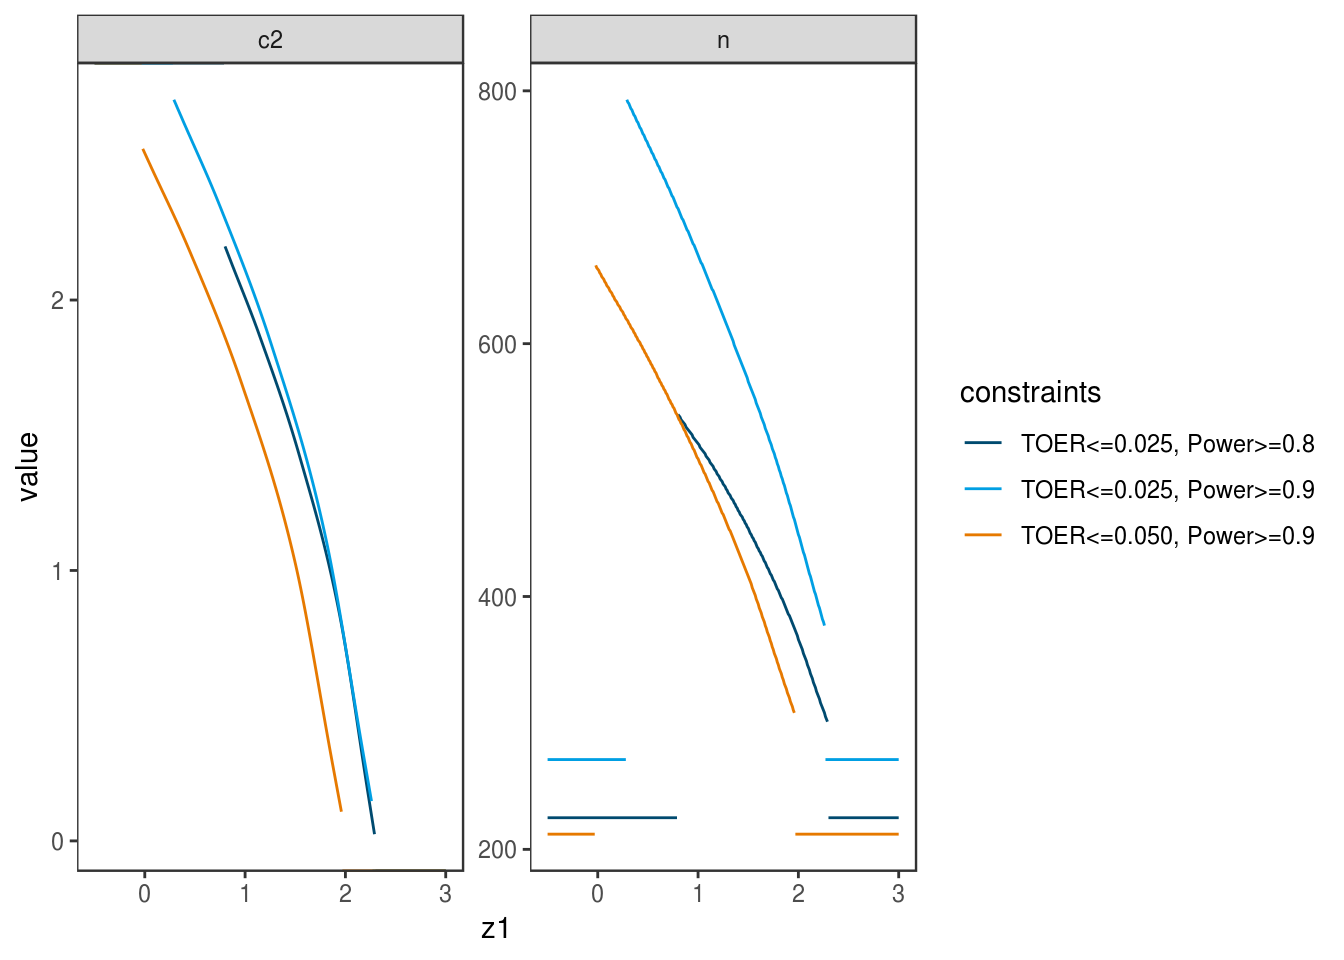
\includegraphics{adoptr-validation-report_files/figure-latex/unnamed-chunk-113-1.pdf}

\hypertarget{scenarioV}{%
\chapter{Scenario V: Single-arm design, medium effect size}\label{scenarioV}}

\hypertarget{details-4}{%
\section{Details}\label{details-4}}

In this scenario, a classical two-arm trial with normal
test statistic and known variance (w.l.o.g. variance of
the test statistic is 1).
This situation corresponds to a classical \(z\)-test for
a difference in population means.

\begin{Shaded}
\begin{Highlighting}[]
\NormalTok{datadist <-}\StringTok{ }\KeywordTok{Normal}\NormalTok{(}\DataTypeTok{two_armed =} \OtherTok{TRUE}\NormalTok{)}
\end{Highlighting}
\end{Shaded}

The null hypothesis is no population mean difference, i.e.
\(\mathcal{H}_0:\delta \leq 0\).

\begin{Shaded}
\begin{Highlighting}[]
\NormalTok{H_}\DecValTok{0}\NormalTok{ <-}\StringTok{ }\KeywordTok{PointMassPrior}\NormalTok{(.}\DecValTok{0}\NormalTok{, }\DecValTok{1}\NormalTok{)}
\end{Highlighting}
\end{Shaded}

An alternative effect size of \(\delta = 0.3\) with
point prior distribution is assumed.

\begin{Shaded}
\begin{Highlighting}[]
\NormalTok{prior <-}\StringTok{ }\KeywordTok{PointMassPrior}\NormalTok{(.}\DecValTok{3}\NormalTok{, }\DecValTok{1}\NormalTok{)}
\end{Highlighting}
\end{Shaded}

Across all variants in this scenario, the one-sided maximal
type one error rate is restricted to

\begin{Shaded}
\begin{Highlighting}[]
\NormalTok{alpha <-}\StringTok{ }\FloatTok{0.025}
\end{Highlighting}
\end{Shaded}

and the power at the point alternative of \(\delta=0.3\) must
be at least

\begin{Shaded}
\begin{Highlighting}[]
\NormalTok{min_power <-}\StringTok{ }\FloatTok{0.8}
\end{Highlighting}
\end{Shaded}

I.e. throughout this sceanrio, we always use the two
constraints

\begin{Shaded}
\begin{Highlighting}[]
\NormalTok{toer_cnstr <-}\StringTok{ }\KeywordTok{expected}\NormalTok{(}\KeywordTok{ConditionalPower}\NormalTok{(datadist, H_}\DecValTok{0}\NormalTok{)) }\OperatorTok{<=}\StringTok{ }\NormalTok{alpha}
\end{Highlighting}
\end{Shaded}

and

\begin{Shaded}
\begin{Highlighting}[]
\NormalTok{pow_cnstr <-}\StringTok{ }\KeywordTok{expected}\NormalTok{(}\KeywordTok{ConditionalPower}\NormalTok{(datadist, prior)) }\OperatorTok{>=}\StringTok{ }\NormalTok{min_power}
\end{Highlighting}
\end{Shaded}

\hypertarget{variantV_1}{%
\section{Variant V-1, sensitivity to integration order}\label{variantV_1}}

\hypertarget{objective-10}{%
\subsection{Objective}\label{objective-10}}

Expected sample size under the respective prior is minimized, i.e.,
\(\boldsymbol{E}\big[n(\mathcal{D})\big]\).

\begin{Shaded}
\begin{Highlighting}[]
\NormalTok{ess <-}\StringTok{ }\KeywordTok{expected}\NormalTok{(}\KeywordTok{ConditionalSampleSize}\NormalTok{(datadist, prior))}
\end{Highlighting}
\end{Shaded}

\hypertarget{constrains-10}{%
\subsection{Constrains}\label{constrains-10}}

No additional constraints are considered in this variant.

\hypertarget{initial-design-9}{%
\subsection{Initial Design}\label{initial-design-9}}

A fixed design for these parameters would require
176
subjects per group. We use the half of this as initial values for the
sample sizes.
The initial stop for futility is at \(c_1^f=0\), i.e., if the effect shows
in the opponent direction to the alternative.
The starting values for the efficacy stop and for \(c_2\) is the \(1-\alpha\)-
quantile of the normal distribution.

\begin{Shaded}
\begin{Highlighting}[]
\NormalTok{init_design <-}\StringTok{ }\ControlFlowTok{function}\NormalTok{(order) \{}
    \KeywordTok{TwoStageDesign}\NormalTok{(}
        \DataTypeTok{n1 =} \KeywordTok{ceiling}\NormalTok{(pwr}\OperatorTok{::}\KeywordTok{pwr.t.test}\NormalTok{(}\DataTypeTok{d =} \FloatTok{.3}\NormalTok{, }
                                     \DataTypeTok{sig.level =} \FloatTok{.025}\NormalTok{, }
                                     \DataTypeTok{power =} \FloatTok{.8}\NormalTok{, }
                                     \DataTypeTok{alternative =} \StringTok{"greater"}\NormalTok{)}\OperatorTok{$}\NormalTok{n) }\OperatorTok{/}\StringTok{ }\DecValTok{2}\NormalTok{,}
        \DataTypeTok{c1f =} \DecValTok{0}\NormalTok{,}
        \DataTypeTok{c1e =} \KeywordTok{qnorm}\NormalTok{( }\DecValTok{1} \OperatorTok{-}\StringTok{ }\FloatTok{0.025}\NormalTok{),}
        \DataTypeTok{n2 =} \KeywordTok{ceiling}\NormalTok{(pwr}\OperatorTok{::}\KeywordTok{pwr.t.test}\NormalTok{(}\DataTypeTok{d =} \FloatTok{.3}\NormalTok{, }
                                     \DataTypeTok{sig.level =} \FloatTok{.025}\NormalTok{, }
                                     \DataTypeTok{power =} \FloatTok{.8}\NormalTok{, }
                                     \DataTypeTok{alternative =} \StringTok{"greater"}\NormalTok{)}\OperatorTok{$}\NormalTok{n) }\OperatorTok{/}\StringTok{ }\DecValTok{2}\NormalTok{,}
        \DataTypeTok{c2 =} \KeywordTok{qnorm}\NormalTok{(}\DecValTok{1} \OperatorTok{-}\StringTok{ }\FloatTok{0.025}\NormalTok{),}
        \DataTypeTok{order =}\NormalTok{ order}
\NormalTok{)}
\NormalTok{\}}
\end{Highlighting}
\end{Shaded}

\hypertarget{optimization-9}{%
\subsection{Optimization}\label{optimization-9}}

The optimal design is computed for three different integration orders: 5, 8,
and 11.

\begin{Shaded}
\begin{Highlighting}[]
\NormalTok{opt_design <-}\StringTok{ }\ControlFlowTok{function}\NormalTok{(order) \{}
    \KeywordTok{minimize}\NormalTok{(}
\NormalTok{        ess,}
        \KeywordTok{subject_to}\NormalTok{(}
\NormalTok{            toer_cnstr,}
\NormalTok{            pow_cnstr}
\NormalTok{        ),}
        \DataTypeTok{initial_design =} \KeywordTok{init_design}\NormalTok{(order),}
        \DataTypeTok{opts =}\NormalTok{ opts}
\NormalTok{    )}
\NormalTok{\}}

\NormalTok{opt1 <-}\StringTok{ }\KeywordTok{lapply}\NormalTok{(}\KeywordTok{c}\NormalTok{(}\DecValTok{5}\NormalTok{, }\DecValTok{8}\NormalTok{, }\DecValTok{11}\NormalTok{), }\ControlFlowTok{function}\NormalTok{(x) }\KeywordTok{opt_design}\NormalTok{(x))}
\end{Highlighting}
\end{Shaded}

\begin{verbatim}
## Warning in minimize(ess, subject_to(toer_cnstr, pow_cnstr), initial_design
## = init_design(order), : initial design is infeasible!

## Warning in minimize(ess, subject_to(toer_cnstr, pow_cnstr), initial_design
## = init_design(order), : initial design is infeasible!

## Warning in minimize(ess, subject_to(toer_cnstr, pow_cnstr), initial_design
## = init_design(order), : initial design is infeasible!
\end{verbatim}

\hypertarget{test-cases-10}{%
\subsection{Test cases}\label{test-cases-10}}

Check if the optimization algorithm converged in all cases.

\begin{Shaded}
\begin{Highlighting}[]
\NormalTok{iters <-}\StringTok{ }\KeywordTok{sapply}\NormalTok{(opt1, }\ControlFlowTok{function}\NormalTok{(x) x}\OperatorTok{$}\NormalTok{nloptr_return}\OperatorTok{$}\NormalTok{iterations)}

\KeywordTok{print}\NormalTok{(iters)}
\end{Highlighting}
\end{Shaded}

\begin{verbatim}
## [1] 2328 4226 8913
\end{verbatim}

\begin{Shaded}
\begin{Highlighting}[]
\NormalTok{testthat}\OperatorTok{::}\KeywordTok{expect_true}\NormalTok{(}\KeywordTok{all}\NormalTok{(iters }\OperatorTok{<}\StringTok{ }\NormalTok{opts}\OperatorTok{$}\NormalTok{maxeval))}
\end{Highlighting}
\end{Shaded}

Check type one error rate control.

\begin{Shaded}
\begin{Highlighting}[]
\NormalTok{tmp     <-}\StringTok{ }\KeywordTok{sapply}\NormalTok{(opt1, }\ControlFlowTok{function}\NormalTok{(x) }\KeywordTok{sim_pr_reject}\NormalTok{(x}\OperatorTok{$}\NormalTok{design, }\FloatTok{.0}\NormalTok{, datadist))}
\NormalTok{df_toer <-}\StringTok{ }\KeywordTok{data.frame}\NormalTok{(}
    \DataTypeTok{toer =} \KeywordTok{as.numeric}\NormalTok{(tmp[}\DecValTok{1}\NormalTok{, ]),}
    \DataTypeTok{se   =} \KeywordTok{as.numeric}\NormalTok{(tmp[}\DecValTok{2}\NormalTok{, ])}
\NormalTok{)}
\KeywordTok{rm}\NormalTok{(tmp)}

\NormalTok{testthat}\OperatorTok{::}\KeywordTok{expect_true}\NormalTok{(}\KeywordTok{all}\NormalTok{(df_toer}\OperatorTok{$}\NormalTok{toer }\OperatorTok{<=}\StringTok{ }\NormalTok{alpha }\OperatorTok{*}\StringTok{ }\NormalTok{(}\DecValTok{1} \OperatorTok{+}\StringTok{ }\NormalTok{tol)))}

\NormalTok{df_toer}
\end{Highlighting}
\end{Shaded}

\begin{verbatim}
##       toer           se
## 1 0.024975 0.0001560489
## 2 0.024956 0.0001559911
## 3 0.024950 0.0001559728
\end{verbatim}

Check the power constraint.

\begin{Shaded}
\begin{Highlighting}[]
\NormalTok{tmp     <-}\StringTok{ }\KeywordTok{sapply}\NormalTok{(opt1, }\ControlFlowTok{function}\NormalTok{(x) }\KeywordTok{sim_pr_reject}\NormalTok{(x}\OperatorTok{$}\NormalTok{design, }\FloatTok{.3}\NormalTok{, datadist))}
\NormalTok{df_pow  <-}\StringTok{ }\KeywordTok{data.frame}\NormalTok{(}
    \DataTypeTok{power =} \KeywordTok{as.numeric}\NormalTok{(tmp[}\DecValTok{1}\NormalTok{, ]),}
    \DataTypeTok{se    =} \KeywordTok{as.numeric}\NormalTok{(tmp[}\DecValTok{2}\NormalTok{, ])}
\NormalTok{)}
\KeywordTok{rm}\NormalTok{(tmp)}

\NormalTok{testthat}\OperatorTok{::}\KeywordTok{expect_true}\NormalTok{(}\KeywordTok{all}\NormalTok{(df_pow}\OperatorTok{$}\NormalTok{pow }\OperatorTok{>=}\StringTok{ }\NormalTok{min_power }\OperatorTok{*}\StringTok{ }\NormalTok{(}\DecValTok{1} \OperatorTok{-}\StringTok{ }\NormalTok{tol)))}

\NormalTok{df_pow}
\end{Highlighting}
\end{Shaded}

\begin{verbatim}
##      power           se
## 1 0.799791 0.0004001569
## 2 0.799696 0.0004002280
## 3 0.799678 0.0004002415
\end{verbatim}

Check expected sample size under the prior.

\begin{Shaded}
\begin{Highlighting}[]
\NormalTok{tmp    <-}\StringTok{ }\KeywordTok{sapply}\NormalTok{(opt1, }\ControlFlowTok{function}\NormalTok{(x) }\KeywordTok{sim_n}\NormalTok{(x}\OperatorTok{$}\NormalTok{design, }\FloatTok{.3}\NormalTok{, datadist))}
\NormalTok{df_ess <-}\StringTok{ }\KeywordTok{data.frame}\NormalTok{(}
    \DataTypeTok{n  =} \KeywordTok{as.numeric}\NormalTok{(tmp[}\DecValTok{1}\NormalTok{, ]),}
    \DataTypeTok{se =} \KeywordTok{as.numeric}\NormalTok{(tmp[}\DecValTok{2}\NormalTok{, ])}
\NormalTok{)}
\KeywordTok{rm}\NormalTok{(tmp)}

\NormalTok{df_ess}
\end{Highlighting}
\end{Shaded}

\begin{verbatim}
##          n         se
## 1 141.9614 0.04874384
## 2 141.9801 0.04875722
## 3 141.9822 0.04875670
\end{verbatim}

\hypertarget{variantV_2}{%
\section{Variant V-2, utility maximization}\label{variantV_2}}

\hypertarget{objective-11}{%
\subsection{Objective}\label{objective-11}}

In this case, a utility function consisting of expected sample size and
power is minimized.

\begin{Shaded}
\begin{Highlighting}[]
\NormalTok{pow <-}\StringTok{ }\KeywordTok{expected}\NormalTok{(}\KeywordTok{ConditionalPower}\NormalTok{(datadist, prior))}

\NormalTok{obj <-}\StringTok{ }\ControlFlowTok{function}\NormalTok{(lambda) \{}
    \KeywordTok{expected}\NormalTok{(}\KeywordTok{ConditionalSampleSize}\NormalTok{(datadist, prior)) }\OperatorTok{+}\StringTok{  }
\StringTok{        }\NormalTok{(}\OperatorTok{-}\NormalTok{lambda) }\OperatorTok{*}\StringTok{ }\NormalTok{pow}
\NormalTok{\}}
\end{Highlighting}
\end{Shaded}

\hypertarget{constrains-11}{%
\subsection{Constrains}\label{constrains-11}}

The type one error rate is controlled at 0.025 on the boundary of the
null hypothesis. Hence, the previous inequality can still be used.
There is no constraint on power anymore because power is part of the
objective utility function.

\hypertarget{initial-design-10}{%
\subsection{Initial Design}\label{initial-design-10}}

The previous initial design with order \(5\) is applied.

\hypertarget{optimization-10}{%
\subsection{Optimization}\label{optimization-10}}

The optimal design is computed for two values of \(\lambda\): 200 and 500.

\begin{Shaded}
\begin{Highlighting}[]
\NormalTok{opt2_design <-}\StringTok{ }\ControlFlowTok{function}\NormalTok{(lambda) \{}

    \KeywordTok{minimize}\NormalTok{(}
        \KeywordTok{obj}\NormalTok{(lambda),}
        \KeywordTok{subject_to}\NormalTok{(}
\NormalTok{            toer_cnstr}
\NormalTok{        ),}
        \DataTypeTok{initial_design =} \KeywordTok{init_design}\NormalTok{(}\DecValTok{5}\NormalTok{),}
        \DataTypeTok{opts =}\NormalTok{ opts}
\NormalTok{    )}
\NormalTok{\}}

\NormalTok{opt2 <-}\StringTok{ }\KeywordTok{lapply}\NormalTok{(}\KeywordTok{c}\NormalTok{(}\DecValTok{200}\NormalTok{, }\DecValTok{500}\NormalTok{), }\ControlFlowTok{function}\NormalTok{(x) }\KeywordTok{opt2_design}\NormalTok{(x))}
\end{Highlighting}
\end{Shaded}

\begin{verbatim}
## Warning in minimize(obj(lambda), subject_to(toer_cnstr), initial_design =
## init_design(5), : initial design is infeasible!

## Warning in minimize(obj(lambda), subject_to(toer_cnstr), initial_design =
## init_design(5), : initial design is infeasible!
\end{verbatim}

\hypertarget{test-cases-11}{%
\subsection{Test cases}\label{test-cases-11}}

Check if the optimization algorithm converged in all cases.

\begin{Shaded}
\begin{Highlighting}[]
\NormalTok{iters <-}\StringTok{ }\KeywordTok{sapply}\NormalTok{(opt2, }\ControlFlowTok{function}\NormalTok{(x) x}\OperatorTok{$}\NormalTok{nloptr_return}\OperatorTok{$}\NormalTok{iterations)}

\KeywordTok{print}\NormalTok{(iters)}
\end{Highlighting}
\end{Shaded}

\begin{verbatim}
## [1]  2062 13606
\end{verbatim}

\begin{Shaded}
\begin{Highlighting}[]
\NormalTok{testthat}\OperatorTok{::}\KeywordTok{expect_true}\NormalTok{(}\KeywordTok{all}\NormalTok{(iters }\OperatorTok{<}\StringTok{ }\NormalTok{opts}\OperatorTok{$}\NormalTok{maxeval))}
\end{Highlighting}
\end{Shaded}

Check type one error rate control for both designs via simulation.

\begin{Shaded}
\begin{Highlighting}[]
\NormalTok{tmp     <-}\StringTok{ }\KeywordTok{sapply}\NormalTok{(opt2, }\ControlFlowTok{function}\NormalTok{(x) }\KeywordTok{sim_pr_reject}\NormalTok{(x}\OperatorTok{$}\NormalTok{design, }\DecValTok{0}\NormalTok{, datadist))}
\NormalTok{df_toer <-}\StringTok{ }\KeywordTok{data.frame}\NormalTok{(}
    \DataTypeTok{toer =} \KeywordTok{as.numeric}\NormalTok{(tmp[}\DecValTok{1}\NormalTok{, ]),}
    \DataTypeTok{se   =} \KeywordTok{as.numeric}\NormalTok{(tmp[}\DecValTok{2}\NormalTok{, ])}
\NormalTok{)}
\KeywordTok{rm}\NormalTok{(tmp)}

\NormalTok{testthat}\OperatorTok{::}\KeywordTok{expect_true}\NormalTok{(}\KeywordTok{all}\NormalTok{(df_toer}\OperatorTok{$}\NormalTok{toer }\OperatorTok{<=}\StringTok{ }\NormalTok{alpha }\OperatorTok{*}\StringTok{ }\NormalTok{(}\DecValTok{1} \OperatorTok{+}\StringTok{ }\NormalTok{tol)))}

\NormalTok{df_toer}
\end{Highlighting}
\end{Shaded}

\begin{verbatim}
##       toer           se
## 1 0.025024 0.0001561980
## 2 0.024983 0.0001560733
\end{verbatim}

Check if the power of the design with higher \(\lambda\) is larger.

\begin{Shaded}
\begin{Highlighting}[]
\NormalTok{testthat}\OperatorTok{::}\KeywordTok{expect_gte}\NormalTok{(}
    \KeywordTok{evaluate}\NormalTok{(pow, opt2[[}\DecValTok{2}\NormalTok{]]}\OperatorTok{$}\NormalTok{design),}
    \KeywordTok{evaluate}\NormalTok{(pow, opt2[[}\DecValTok{1}\NormalTok{]]}\OperatorTok{$}\NormalTok{design)}
\NormalTok{)}
\end{Highlighting}
\end{Shaded}

Finally the three designs computed so far are plotted together to allow
comparison.

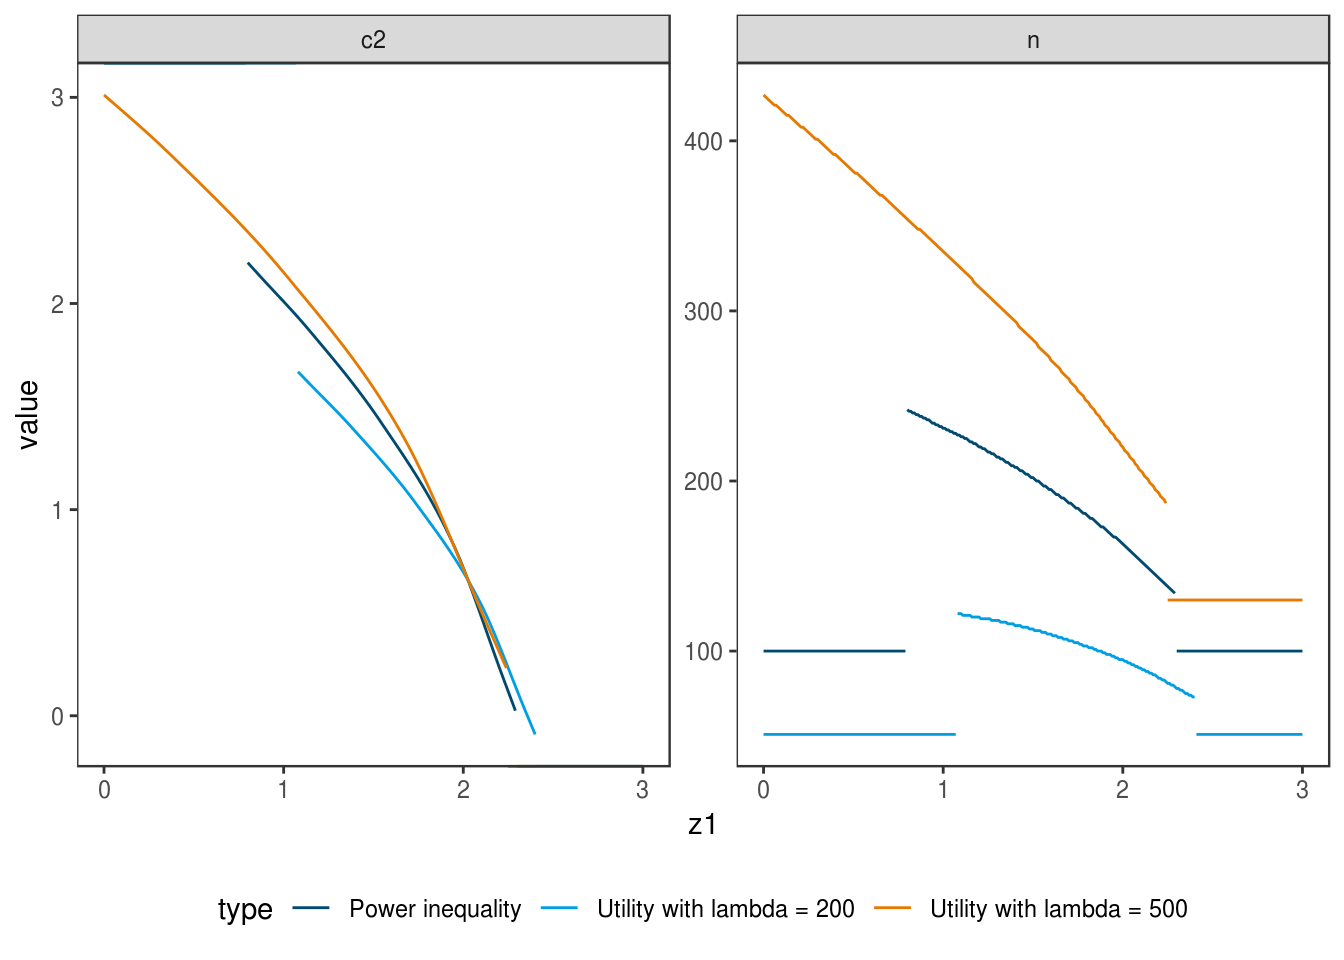
\includegraphics{adoptr-validation-report_files/figure-latex/unnamed-chunk-133-1.pdf}

\hypertarget{variantV_3}{%
\section{Variant V-3, n1-penalty}\label{variantV_3}}

In this case, the influence of the regularization term \texttt{N1()} is investigated.

\hypertarget{objective-12}{%
\subsection{Objective}\label{objective-12}}

In this case, a mixed criterion consisting of expected sample size and
\(n_1\) is minimized.

\begin{Shaded}
\begin{Highlighting}[]
\NormalTok{N1 <-}\StringTok{ }\KeywordTok{N1}\NormalTok{()}

\NormalTok{obj3 <-}\StringTok{ }\ControlFlowTok{function}\NormalTok{(lambda) \{}
\NormalTok{    ess }\OperatorTok{+}\StringTok{ }\NormalTok{lambda }\OperatorTok{*}\StringTok{ }\NormalTok{N1}
\NormalTok{\}}
\end{Highlighting}
\end{Shaded}

\hypertarget{constrains-12}{%
\subsection{Constrains}\label{constrains-12}}

The inequalities from variant V.1 can still be used.

\hypertarget{initial-design-11}{%
\subsection{Initial Design}\label{initial-design-11}}

The previous initial design with order \(5\) is applied.

\hypertarget{optimization-11}{%
\subsection{Optimization}\label{optimization-11}}

The optimal design is computed for two values of \(\lambda\): 0.05 and 0.2.

\begin{Shaded}
\begin{Highlighting}[]
\NormalTok{opt3_design <-}\StringTok{ }\ControlFlowTok{function}\NormalTok{(lambda) \{}

    \KeywordTok{minimize}\NormalTok{(}
        \KeywordTok{obj3}\NormalTok{(lambda),}
        \KeywordTok{subject_to}\NormalTok{(}
\NormalTok{            toer_cnstr,}
\NormalTok{            pow_cnstr}
\NormalTok{        ),}
        \DataTypeTok{initial_design =} \KeywordTok{init_design}\NormalTok{(}\DecValTok{5}\NormalTok{),}
        \DataTypeTok{opts =}\NormalTok{ opts}
\NormalTok{    )}
\NormalTok{\}}

\NormalTok{opt3 <-}\StringTok{ }\KeywordTok{lapply}\NormalTok{(}\KeywordTok{c}\NormalTok{(.}\DecValTok{05}\NormalTok{, }\FloatTok{.2}\NormalTok{), }\ControlFlowTok{function}\NormalTok{(x) }\KeywordTok{opt3_design}\NormalTok{(x))}
\end{Highlighting}
\end{Shaded}

\begin{verbatim}
## Warning in minimize(obj3(lambda), subject_to(toer_cnstr, pow_cnstr),
## initial_design = init_design(5), : initial design is infeasible!

## Warning in minimize(obj3(lambda), subject_to(toer_cnstr, pow_cnstr),
## initial_design = init_design(5), : initial design is infeasible!
\end{verbatim}

\hypertarget{test-cases-12}{%
\subsection{Test cases}\label{test-cases-12}}

Check if the optimization algorithm converged in all cases.

\begin{Shaded}
\begin{Highlighting}[]
\NormalTok{iters <-}\StringTok{ }\KeywordTok{sapply}\NormalTok{(opt3, }\ControlFlowTok{function}\NormalTok{(x) x}\OperatorTok{$}\NormalTok{nloptr_return}\OperatorTok{$}\NormalTok{iterations)}

\KeywordTok{print}\NormalTok{(iters)}
\end{Highlighting}
\end{Shaded}

\begin{verbatim}
## [1] 2233 2478
\end{verbatim}

\begin{Shaded}
\begin{Highlighting}[]
\NormalTok{testthat}\OperatorTok{::}\KeywordTok{expect_true}\NormalTok{(}\KeywordTok{all}\NormalTok{(iters }\OperatorTok{<}\StringTok{ }\NormalTok{opts}\OperatorTok{$}\NormalTok{maxeval))}
\end{Highlighting}
\end{Shaded}

Check if the n1 regularizer of the design with higher \(\lambda\) is lower.

\begin{Shaded}
\begin{Highlighting}[]
\NormalTok{testthat}\OperatorTok{::}\KeywordTok{expect_lte}\NormalTok{(}
    \KeywordTok{evaluate}\NormalTok{(N1, opt3[[}\DecValTok{2}\NormalTok{]]}\OperatorTok{$}\NormalTok{design),}
    \KeywordTok{evaluate}\NormalTok{(N1, opt3[[}\DecValTok{1}\NormalTok{]]}\OperatorTok{$}\NormalTok{design)}
\NormalTok{)}


\NormalTok{testthat}\OperatorTok{::}\KeywordTok{expect_lte}\NormalTok{(}
    \KeywordTok{evaluate}\NormalTok{(N1, opt3[[}\DecValTok{1}\NormalTok{]]}\OperatorTok{$}\NormalTok{design),}
    \KeywordTok{evaluate}\NormalTok{(N1, opt1[[}\DecValTok{1}\NormalTok{]]}\OperatorTok{$}\NormalTok{design)}
\NormalTok{)}
\end{Highlighting}
\end{Shaded}

Finally the three designs computed so far are plotted together to allow
comparison.

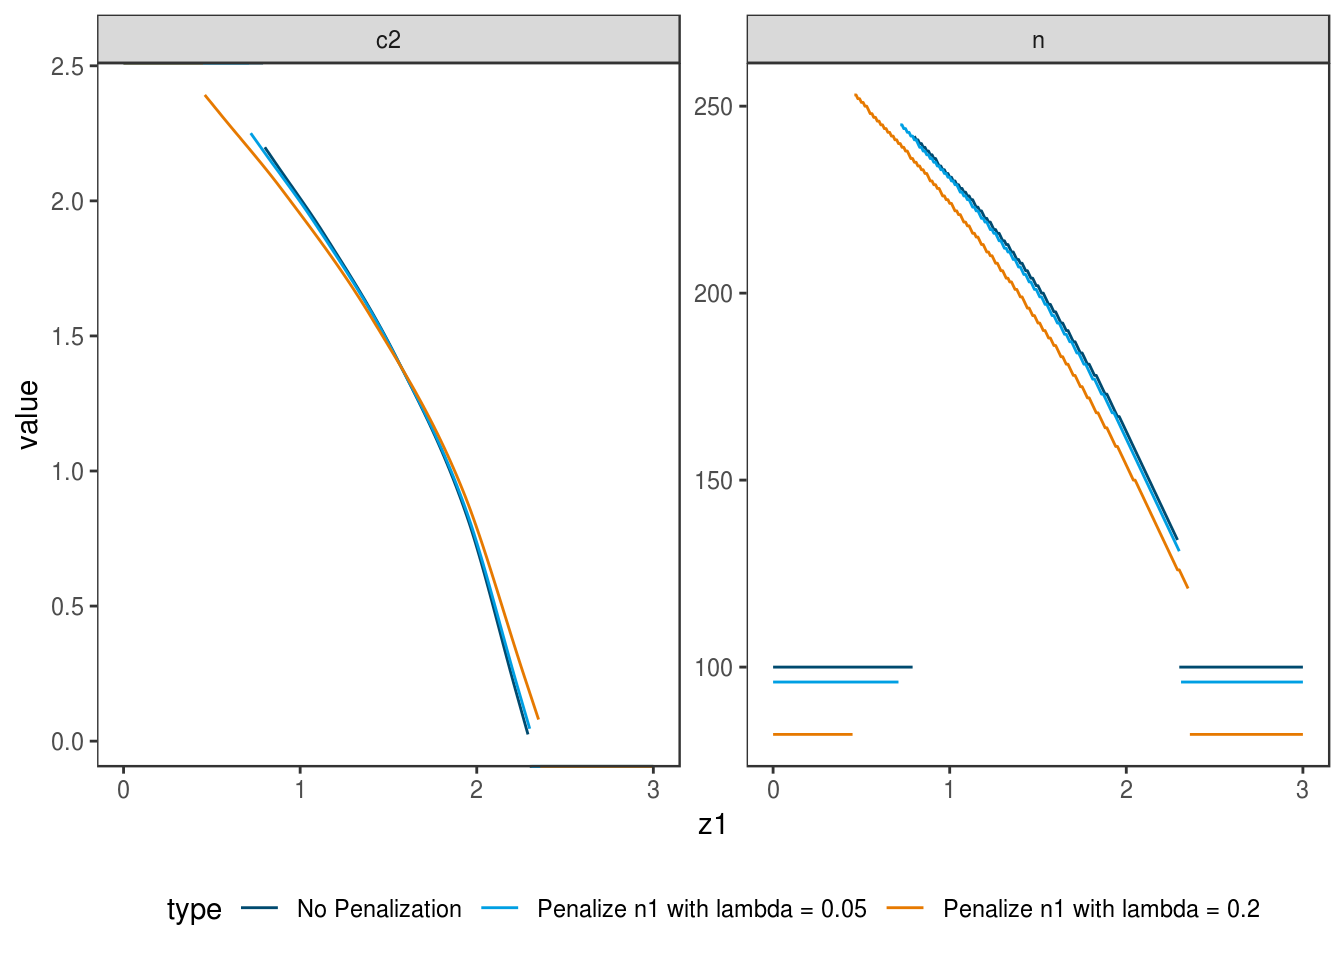
\includegraphics{adoptr-validation-report_files/figure-latex/unnamed-chunk-138-1.pdf}

\hypertarget{variantV_4}{%
\section{Variant V-4, n2-penalty}\label{variantV_4}}

In this case the average over \(n_2\) is penalized by the predefined score
\texttt{AverageN2}.

\hypertarget{objective-13}{%
\subsection{Objective}\label{objective-13}}

In this case, a mixed criterion consisting of expected sample size and
average of \(n_2\) is minimized.

\begin{Shaded}
\begin{Highlighting}[]
\NormalTok{avn2 <-}\StringTok{ }\KeywordTok{AverageN2}\NormalTok{()}

\NormalTok{obj4 <-}\StringTok{ }\ControlFlowTok{function}\NormalTok{(lambda) \{}
\NormalTok{    ess }\OperatorTok{+}\StringTok{ }\NormalTok{lambda }\OperatorTok{*}\StringTok{ }\NormalTok{avn2}
\NormalTok{\}}
\end{Highlighting}
\end{Shaded}

\hypertarget{constrains-13}{%
\subsection{Constrains}\label{constrains-13}}

The inequalities from variant V.1 can still be used.

\hypertarget{initial-design-12}{%
\subsection{Initial Design}\label{initial-design-12}}

The previous initial design with order \(5\) is applied.

\hypertarget{optimization-12}{%
\subsection{Optimization}\label{optimization-12}}

The optimal design is computed for two values of \(\lambda\): 0.01 and 0.1.

\begin{Shaded}
\begin{Highlighting}[]
\NormalTok{opt4_design <-}\StringTok{ }\ControlFlowTok{function}\NormalTok{(lambda) \{}
    \KeywordTok{minimize}\NormalTok{(}
        \KeywordTok{obj4}\NormalTok{(lambda),}
        \KeywordTok{subject_to}\NormalTok{(}
\NormalTok{            toer_cnstr,}
\NormalTok{            pow_cnstr}
\NormalTok{        ),}
        \DataTypeTok{initial_design =} \KeywordTok{init_design}\NormalTok{(}\DecValTok{5}\NormalTok{),}
        \DataTypeTok{upper_boundary_design =} \KeywordTok{get_upper_boundary_design}\NormalTok{(}\KeywordTok{init_design}\NormalTok{(}\DecValTok{5}\NormalTok{), }\DataTypeTok{c2_buffer=}\DecValTok{3}\NormalTok{),}
        \DataTypeTok{opts =}\NormalTok{ opts}
\NormalTok{    )}
\NormalTok{\}}

\NormalTok{opt4 <-}\StringTok{ }\KeywordTok{lapply}\NormalTok{(}\KeywordTok{c}\NormalTok{(.}\DecValTok{01}\NormalTok{, }\FloatTok{.1}\NormalTok{), }\ControlFlowTok{function}\NormalTok{(x) }\KeywordTok{opt4_design}\NormalTok{(x))}
\end{Highlighting}
\end{Shaded}

\begin{verbatim}
## Warning in minimize(obj4(lambda), subject_to(toer_cnstr, pow_cnstr),
## initial_design = init_design(5), : initial design is infeasible!

## Warning in minimize(obj4(lambda), subject_to(toer_cnstr, pow_cnstr),
## initial_design = init_design(5), : initial design is infeasible!
\end{verbatim}

\hypertarget{test-cases-13}{%
\subsection{Test cases}\label{test-cases-13}}

Check if the optimization algorithm converged in all cases.

\begin{Shaded}
\begin{Highlighting}[]
\NormalTok{iters <-}\StringTok{ }\KeywordTok{sapply}\NormalTok{(opt4, }\ControlFlowTok{function}\NormalTok{(x) x}\OperatorTok{$}\NormalTok{nloptr_return}\OperatorTok{$}\NormalTok{iterations)}

\KeywordTok{print}\NormalTok{(iters)}
\end{Highlighting}
\end{Shaded}

\begin{verbatim}
## [1] 2196 2376
\end{verbatim}

\begin{Shaded}
\begin{Highlighting}[]
\NormalTok{testthat}\OperatorTok{::}\KeywordTok{expect_true}\NormalTok{(}\KeywordTok{all}\NormalTok{(iters }\OperatorTok{<}\StringTok{ }\NormalTok{opts}\OperatorTok{$}\NormalTok{maxeval))}
\end{Highlighting}
\end{Shaded}

Check if the average \(n_2\) regularizer of the design with
higher \(\lambda\) is lower.

\begin{Shaded}
\begin{Highlighting}[]
\NormalTok{testthat}\OperatorTok{::}\KeywordTok{expect_lte}\NormalTok{(}
    \KeywordTok{evaluate}\NormalTok{(avn2, opt4[[}\DecValTok{2}\NormalTok{]]}\OperatorTok{$}\NormalTok{design),}
    \KeywordTok{evaluate}\NormalTok{(avn2, opt4[[}\DecValTok{1}\NormalTok{]]}\OperatorTok{$}\NormalTok{design)}
\NormalTok{)}


\NormalTok{testthat}\OperatorTok{::}\KeywordTok{expect_lte}\NormalTok{(}
    \KeywordTok{evaluate}\NormalTok{(avn2, opt4[[}\DecValTok{1}\NormalTok{]]}\OperatorTok{$}\NormalTok{design),}
    \KeywordTok{evaluate}\NormalTok{(avn2, opt1[[}\DecValTok{1}\NormalTok{]]}\OperatorTok{$}\NormalTok{design)}
\NormalTok{)}
\end{Highlighting}
\end{Shaded}

Finally the three designs computed so far are plotted together to allow
comparison.

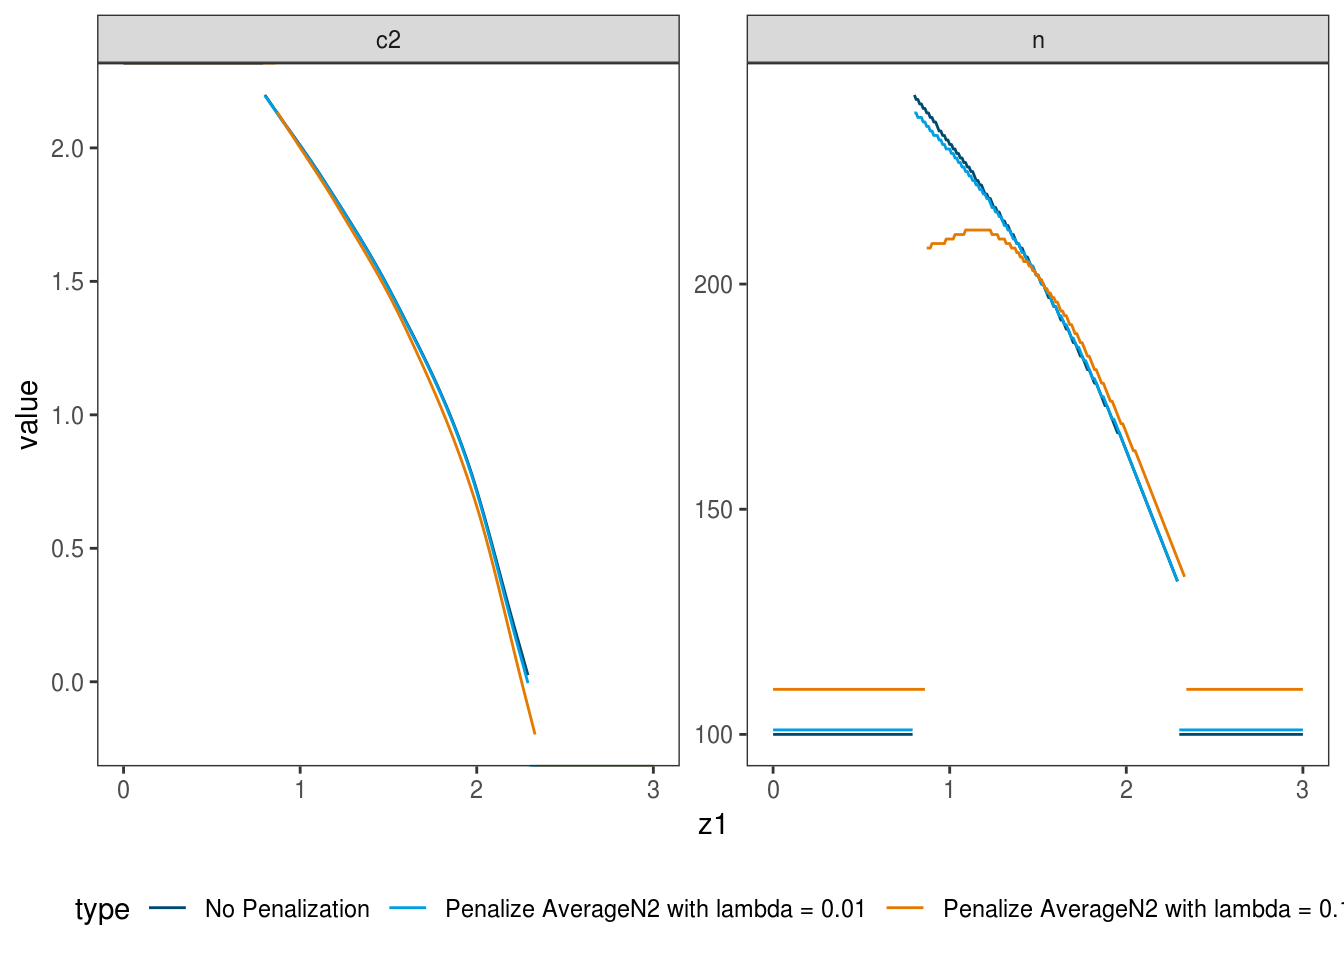
\includegraphics{adoptr-validation-report_files/figure-latex/unnamed-chunk-143-1.pdf}

\bibliography{book.bib,packages.bib}


\end{document}
